
\newpage

\chapter[REFERENCIAL TEORICO]{REFERENCIAL TEÓRICO}
\section{CONTEXTO FINANCEIRO}
\subsection{Mercado Financeiro}

Em um ambiente capitalista há o interesse em aplicar recursos financeiros em troca de remuneração. Quando uma pessoa, física ou jurídica, que consome menos do que produz, tornando-se um agente superavitário, deseja investir os valores excedentes, ela procura por outra pessoa, jurídica, que tenha o interesse em captar esses valores em troca de uma remuneração. Essa remuneração é uma taxa de juros que pode ser previamente definida ou não. Assim, quando há pessoas disponibilizando valores e há em contra parte pessoas comprando esses valores, forma-se então um Mercado Financeiro (IMPORTÂNCIA do Mercado Financeiro, 2013).

Segundo a CVM, Comissão de Valores Mobiliários, o Mercado Financeiro brasileiro é composto por 4 grandes mercados,\cite[p. 15]{cmv2014}, como ilustrado na Figura 1 \ref{f01} e brevemente apresentados nos parágrafos seguintes.

\begin{figure}[h]
\centering
\label{f01}
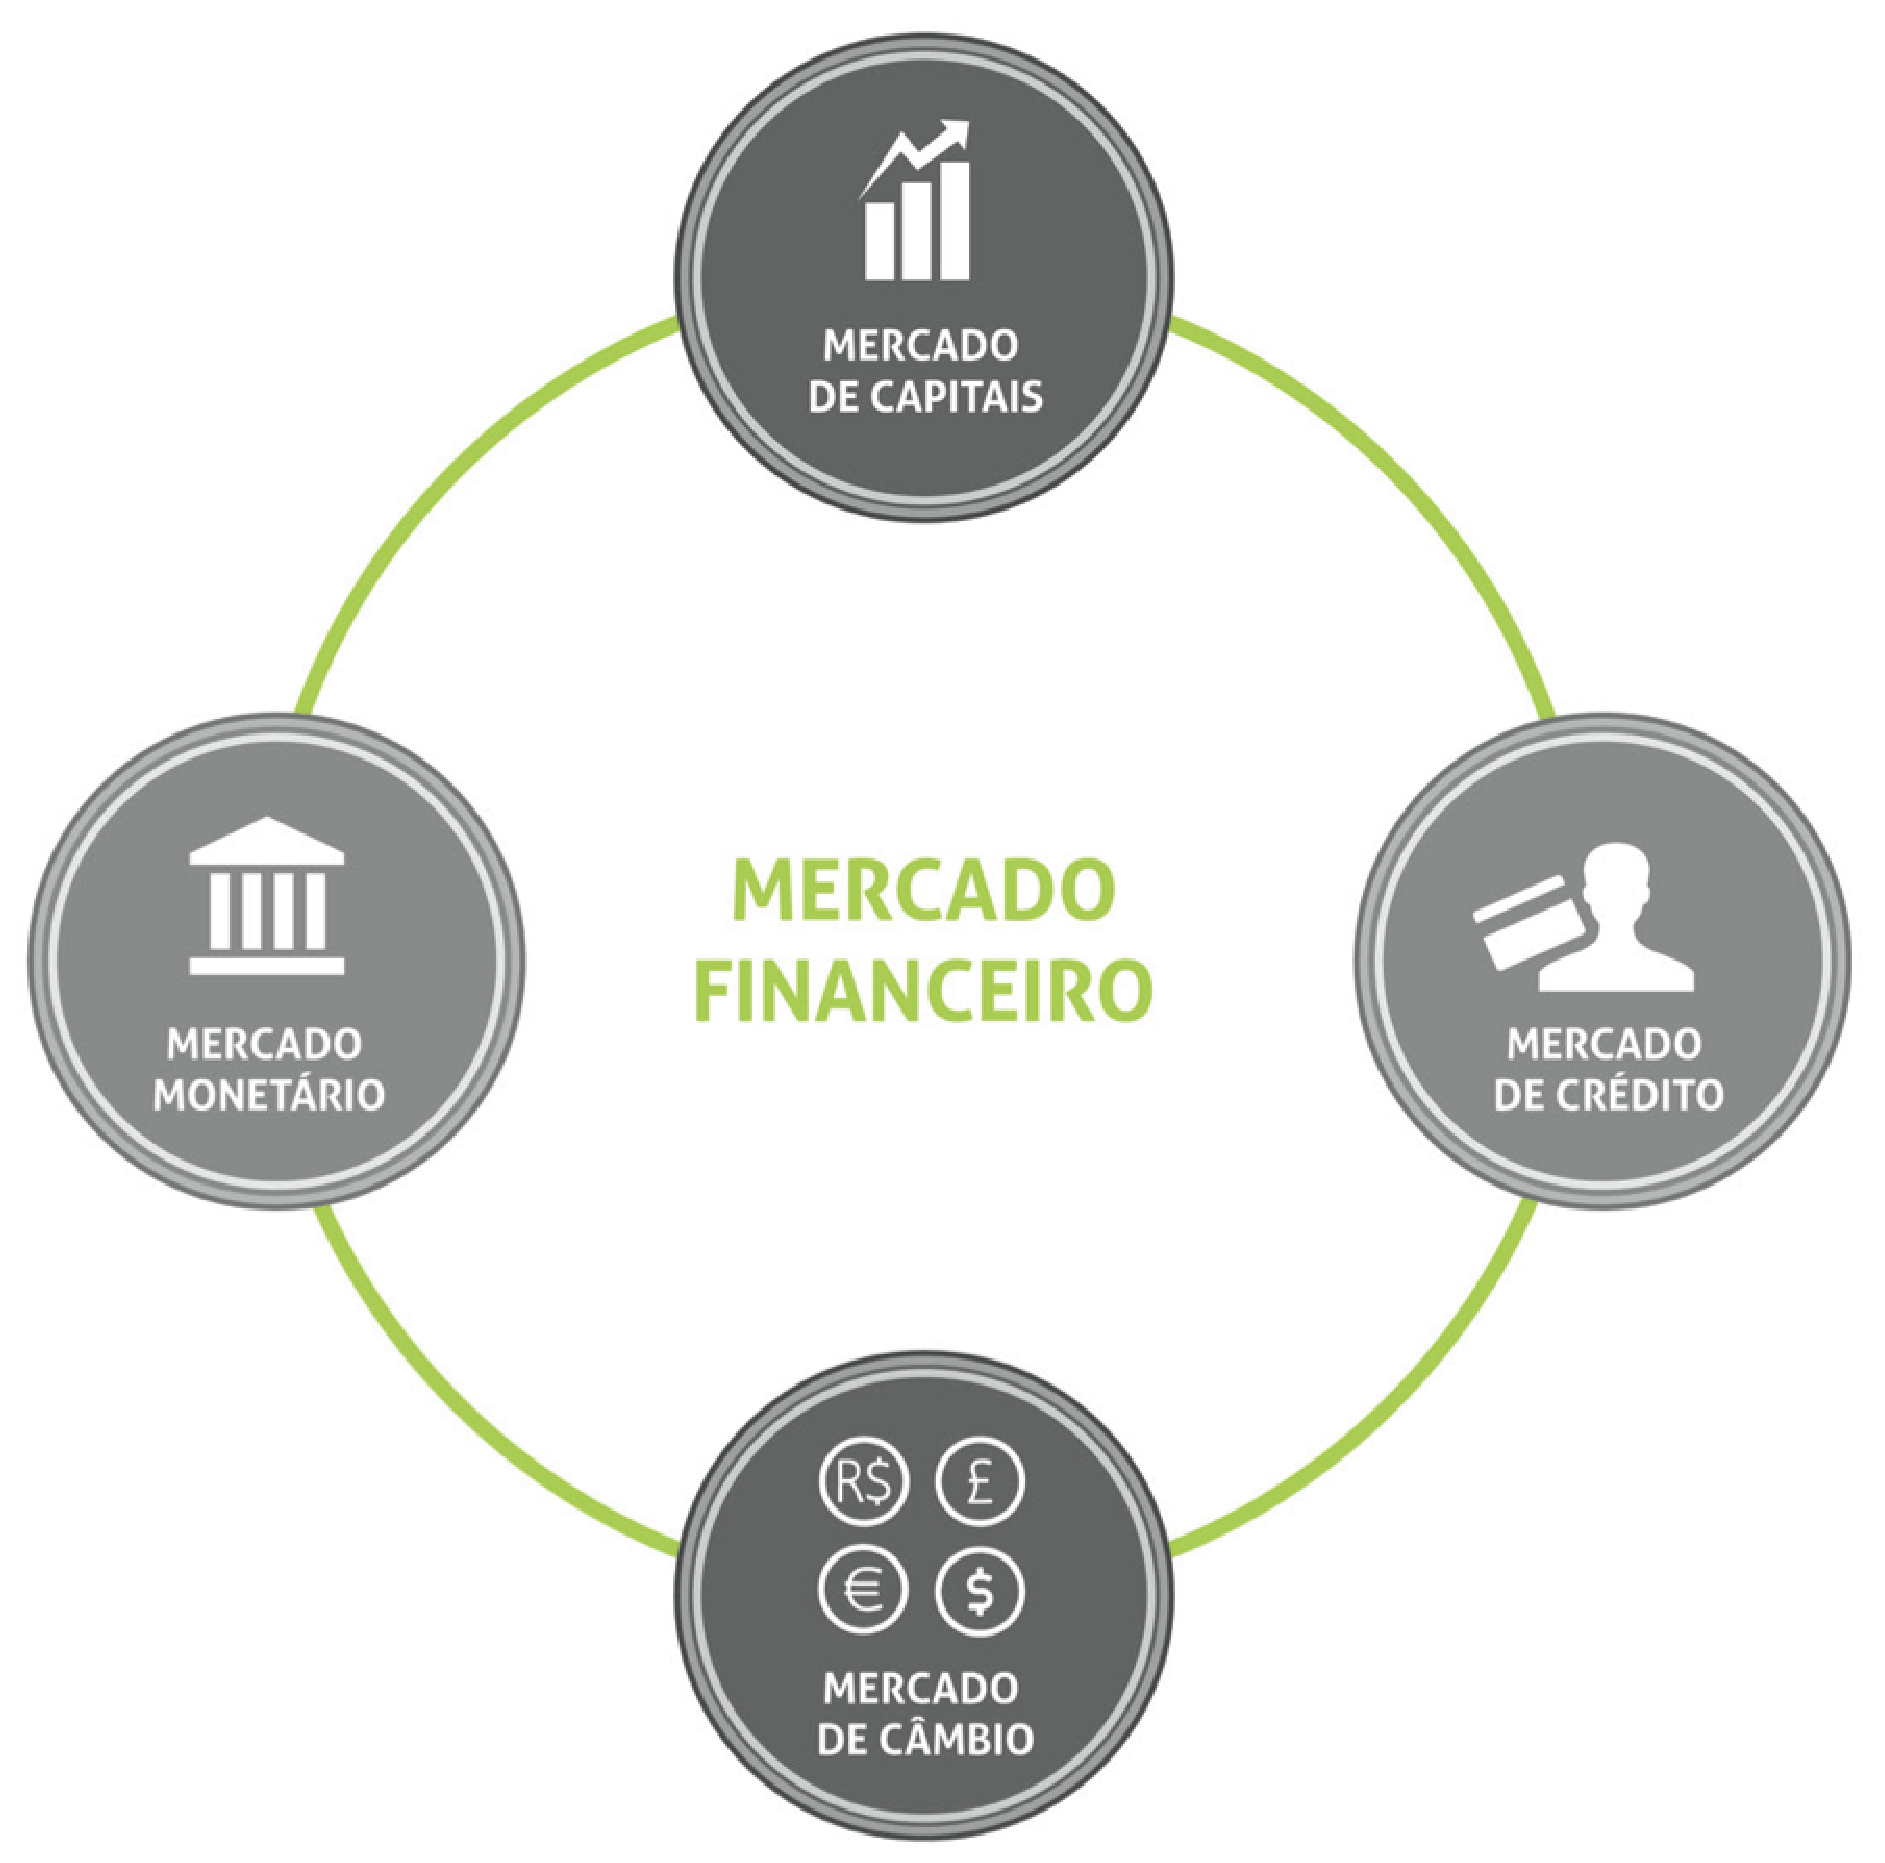
\includegraphics[width=0.5\textwidth]{figuras/f01}
\caption{Composição Mercado Financeiro Brasileiro  \newline fonte: CVM,2013}

\end{figure}

\textbf{Figura 1: }

O Mercado Monetário é um mercado onde os participantes são instituições financeiras, nas quais há diversas transferências de valores em curto prazo, cerca de um dia. Essas transferências são realizadas entre elas e/ou entre elas e o Banco Central, Bacen. O Banco Central, por sua vez, realiza intervenções neste mercado, visando realizar controles em concordância com a Política Monetária Nacional. Política essa que influencia diretamente no controle inflacionário da economia \cite[p. 32]{cmv2014}.

O Mercado de Crédito é o mercado onde instituições financeiras captam dinheiro de agentes superavitários e realizam empréstimos a pessoas físicas ou jurídicas. Esta instituição tem um compromisso com o agente superavitário comprovado por títulos privados. Ao emprestar um valor à uma pessoa, esta instituição financeira é remunerada com a diferença de juros que cobra do devedor e paga ao seu credor (agente superavitário), denominado spread, pelos serviços de intermediação. O Bacen é o principal órgão regulador deste mercado para evitar que ocorram casos de lucros abusivos \cite[p. 32]{cmv2014}.

O Mercado de Câmbio é um mercado onde há transações entre moedas estrangeiras e a moeda nacional. Participam deste mercado instituições que possuem despesas ou receitas em moeda estrangeira. O Bacen é o órgão que regula este mercado visando mantê-lo em concordância com a Política Cambial\cite[p. 32]{cmv2014}.

O Mercado de Capitais é o mercado onde empresas captam valores diretamente com os agentes superavitários, através de títulos como Debêntures, notas promissórias, ações, dentre outros. Em outras palavras, o risco da operação é assumido pelo agente superavitário e não mais pela instituição que faz a intermediação, como no Mercado de Crédito. Porém, essa captação é assessorada por uma empresa apropriada que presta estes serviços. Este mercado é regulado pela CVM (\citeyear{cmv2014},p 33).Os participantes deste mercado estão apresentados no tópico subsequente, uma vez que este será o mercado abordando neste TCC.

\subsection{Mercado Capitais}

Suponha que uma empresa, cujo nome fantasia seria XPTO S.A, tenha interesse em fazer alguns investimentos em seus projetos. Essa empresa poderá financiar seus investimentos de três maneiras: (i) usando recursos próprios atravésdo lucro acumulado ao longo do tempo; (ii) com base em financiamentos de instituições especializadas em venda de crédito; (iii) ou mesmo através do mercado de capitais, com emissão pública de títulos.
	
Ao optar pela terceira alternativa, a empresa deverá iniciar, junto com a CVM, um processo de abertura de capital. Depois, deverá atender os critérios estipulados por essa comissão reguladora. Por fim, poderá disponibilizar publicamente suas ações  em um Mercado de Capitais. 

Ao conseguir a abertura de capital autorizada pela CVM, a empresa emite ações que são adquiridas pelos agentes superavitários, os quais podem ser chamados de investidores, por intermédio de corretoras de valores devidamente registradas. Essas últimas, por sua vez, enviam esses valores à Bolsa de valores, na qual se encontra a ação disponível. No Brasil, a Empresa responsável por promover um ambiente transparente e líquido para realização dessas negociações é a BM\&FBovespa, sediada na capital do Estado de São Paulo.

Para realizar negociações de valores mobiliários, um investidor pode ou não seguir alguma estratégia, que por sua vez pode ou não ser baseada em estudos de especialistas. Estes estudos dividem a atividade de análise de mercado em duas abordagens: a Análise Técnica \cite{noronha2010} e a Análise Fundamentalista \cite{buffet2010}, de um ativo, ambas aplicadas ao Mercado de Ações .

Na abordagem da Análise Técnica, são considerados apenas dados como preço e volume da ação. Em posse destas informações, o analista elabora gráficos, realiza diversos cálculos, usa indicadores matemáticos no intuito de detectar padrões comportamentais do mercado. Vale observar que nesta abordagem não importa de qual empresa pertence a ação, pois o analista deseja encontrar somente os padrões comportamentais dos investidores, para assim elaborar estratégias que retornem o maior lucro possível.

Na abordagem da Análise Fundamentalista, são considerados dados como: (i) Lucro bruto/Margem de lucro bruto; (ii) despesas operacionais; (iii) despesas; (iv) balanço patrimonial  entre outros \cite{buffet2010}. O analista realiza cálculos para encontrar o preço justo da ação desta empresa e o confronta com o valor corrente no mercado, assim realiza operações de compra e/ou venda quando o suas estratégias indicam o melhor momento para operar. Diferente do analista técnico, é importante para o analista fundamentalista conhecer a empresa investida.

Serão adotadas, neste TCC, técnicas financeiras pertencentes à abordagem da Análise Técnica. Técnicas estas desenvolvidas por especialistas no mercado de capitais e publicadas em mídia impressa e/ou virtual.


\section{ENGENHARIA DE SOFTWARE}
\subsection{Sistemas Multagentes}
\subsubsection{Agentes}

Russel e Norving (\citeyear{russel2003}, p. 31) definem: \textit{“An agent is anything that can be viewed as perceiving its environment through sensors and acting upon that environment through actuators”}.Em outras palavras, um agente é capaz de se comportar em um determinado ambiente de acordo com as informações oriundas deste ambiente, seja ele determinístico ou não.

Segundo Wooldridge, um agente possui as seguintes características: (i) Autonomia, não há intervenções no processo de decisão de um agente. Ele toma decisões sem intervenções de outros agentes ou humanos; (ii) Sociabilidade, um agente interage com outros agentes, Software ou humano, através de algum tipo de linguagem de comunicação de agentes, e têm a habilidade de trabalhar em conjuntos com outros agentes afim de alcançar um objetivo; (iii) Reatividade, um agente fica situado em um ambiente e é capaz de perceber esse ambiente através de seus sensores, é capaz de responder em tempo hábil as mudanças que ocorrem nele; e (iv) Pro-atividade, um agente não apenas responde as mudanças do ambiente, ele é capaz de tomar iniciativa \cite[p. 2-3]{wooldrige2002}.

De acordo com Girardi (\citeyear{girardi2004}, p. 5), o mecanismo utilizado para a tomada de decisão da ação a ser executada a partir de uma percepção é o que distingue um agente, classificando-o em um agente: (i) deliberativo, quando a tomada de decisão da ação a ser executada é realizada via raciocínio lógico em concordância com um plano de ações para atingir alguma meta; (ii) reativo, quando o agente não possui um modelo do ambiente, agindo apenas em reposta a estímulos do ambiente na qual está inserido, sendo assim, um agente reativo não conhece o ambiente ao qual pertence; e (iii) camadas, quando um agente possui características de um agente deliberativo e de um agente reativo \cite[p. 5]{girardi2004}. 

\subsubsubsection{Agentes Comportamentais}

Um agente comportamental é um agente reativo,que tem seus comportamento abstraídos de comportamentos de uma entidade do mundo real, normalmente \cite[p. 33]{oliveira2008}. Um conjunto de agentes comportamentais, de maneira cooperativa, pode ser utilizado para solucionar um problema complexo. Um exemplo comumente encontrado na literatura, é o da colônia de formigas. Neste cenário cada formiga é uma entidade simples, mas em conjunto é capaz de realizartrabalhos complexos existentes em uma colônia, por exemplo: construir um formigueiro semelhante ao da Figura 2(\ref{f02}).

\begin{figure}[h]
\centering
\label{f02}
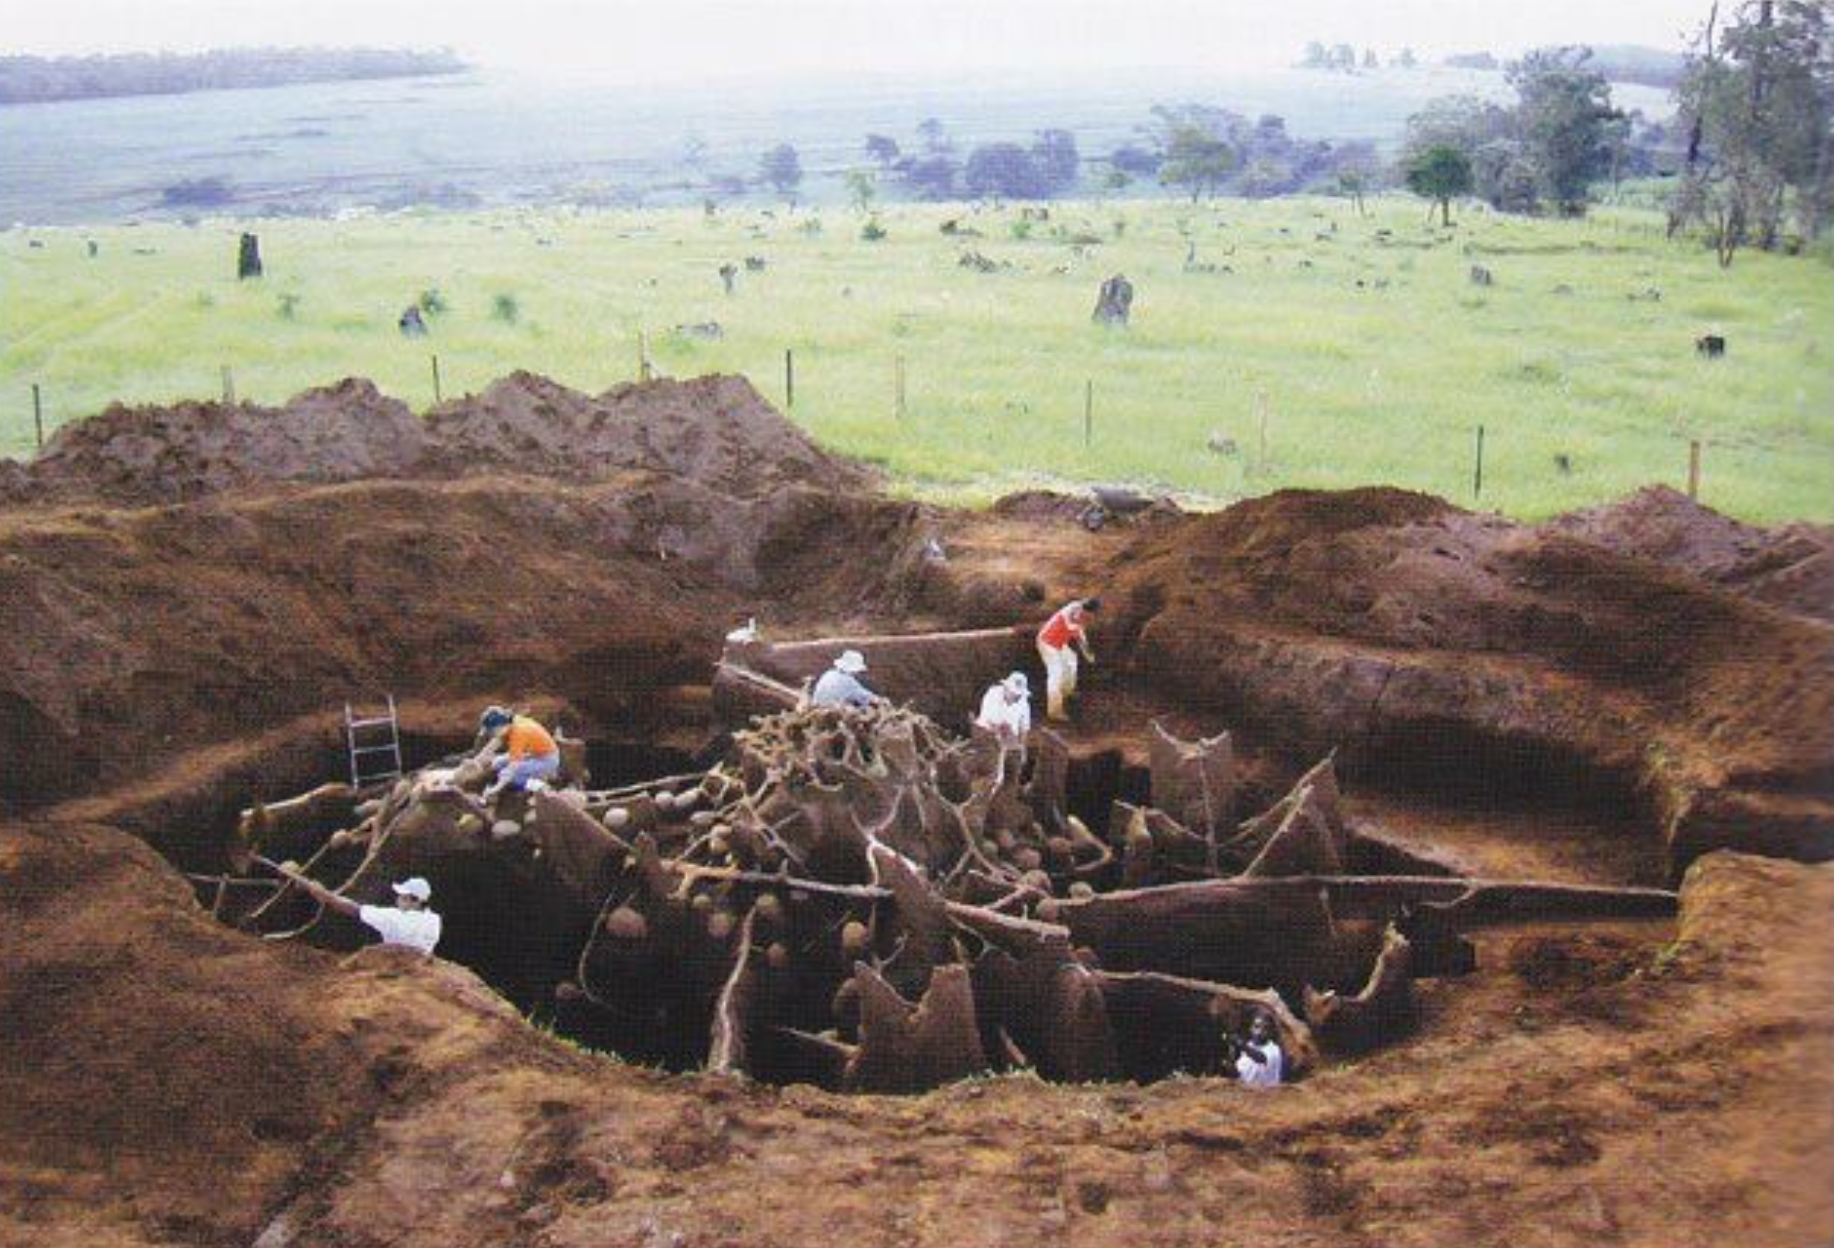
\includegraphics[width=0.5\textwidth]{figuras/f02}
\caption{Formigueiro }

\end{figure}

As formigas são dividas por tipos de trabalhos, assim temos as seguintes entidades, ou agentes comportamentais: (i) Rainhas, formigas responsáveis por pôr ovos que darão origem a novas formigas da colônia; (ii) Operárias, formigas que realizam tarefas de acordo com a sua idade e tamanho; (iii) Machos, formigas que vivem apenas o suficiente para fecundar a Rainha. Em uma colônia, as formigas Operárias mais novas e menores ficam responsáveis por atividades de alimentar a Rainha e lavas, e de limpeza do formigueiro. Já para as operárias mais velhas, ficam as atividades de maior risco, como a proteção do formigueiro (para formigas maiores) e a busca por novas fontes externas de alimento \apud[p. 35]{holldobler1990} {oliveira2008}.

Alvares e Sichman (\citeyear{alvares1997}, p. 12) destacam do exemplo das formigas características dos sistemas multiagentes reativos:

\begin{citacao}
\begin{enumerate}

	\item Não há representação explícita de conhecimento- o conhecimento dos agentes é implícito e se manifesta através do seu comportamento;

	\item Não há representação do ambiente- o seu comportamento se baseia no que é percebido a cada instante do ambiente, mas sem uma representação explicita deste; 

	\item Não há memória das ações – o agentes reativos não mantém um histórico de suas ações, de forma que o resultado de uma ação passada não exerce nenhuma influência sobre as suas ações futuras;


	\item Organização etológica – a forma de organização dos agentes reativos é similar a dos animais, em oposição à organização social dos sistemas cognitivos;

 	\item Grande número de membros – os sistemas multiagentes reativos têm, em geral, um grande número de agentes, da ordem de dezenas, centenas ou mesmo milhões de agentes.
 	\newline \cite[p. 12]{alvares1997}.

\end{enumerate}
\end{citacao}


\subsubsubsection{Agentes Intencionais}

Quando um aluno deixa a universidade com uma primeira graduação, ele se depara com uma decisão a tomar, sobre o que fazer com sua vida. O processo de decisão tipicamente inicia-se tentando se entender as opções que se tem disponíveis em função do conhecimento (crenças) que o aluno possui do seu ambiente. Por exemplo, se o aluno tem um bom histórico escolar, então uma opção é se tornar um acadêmico. Outra opção é se tornar um profissional. Após a geração do grupo de alternativas (desejos), deve-se optar por uma e se comprometer com ela. Esta escolha vem a ser sua intenção. As intenções alimentam o raciocínio lógico futuro do agente. Por exemplo, se o aluno decidir que quer se tornar um acadêmico, então ele deve comprometer-se com esse objetivo e despender tempo e esforço para alcançá-lo. \apud[p. 4] {wooldridge1999}{girardi2004}.

Agentes deliberativos são agentes capazes de decidir de maneira autônoma seus objetivos e os mudar no decorrer do tempo. Ou seja, estes agentes apresentam uma considerável capacidade cognitiva. Agentes deliberativos possuem as seguintes características:
\begin{citacao}
\begin{enumerate}

	\item Mantêm uma representação explicita de seu ambiente e dos outros agentes;
	\item Podem manter um histórico das interações e ações passadas, isto é, têm memória do passado;
	\item A comunicação entre os agentes é feita de modo direto, através do envio e recebimento de mensagens;
	\item Seu mecanismo de controle é deliberativo, ou seja, tais agentes raciocinam sobre quais objetivos devem alcançar, quais planos seguir e quais ações devem ser executadas num determinado momento;
	\item Seu modelo de organização é baseado em modelos sociológicos, como organizações humanas;
	\item Uma sociedade contém tipicamente poucos agentes, na ordem de uma dezena.
	 \newline \apud[p. 28]{ferber1991}{alvares1997}

\end{enumerate}
\end{citacao}

Um modelo de agente deliberativobastante investigado na Inteligência Artificial é o modelo Belief-Desire-Intention (BDI) \apud[p. 30]{bratman1999}{serrano2011}.Neste modelo, o raciocínio humano é representado através de crenças, desejos e intenções. As crenças formam o conhecimento do agente, e estas são abstrações de informações do mundo real. Os desejos são as metas do agente, são a razão por trás das ações dos agentes. As intenções são as ações do agente, são as sequência de tarefas que o agente desempenha para atender um desejo que é criado por suas crenças \cite[p. 31]{serrano2011}.

\subsubsection{Sistemas Multiagentes (SMA)}

Girardi (\citeyear{girardi2004}, p.6) caracteriza um sistema multiagentes (SMA) como \textit{“um grupo de agentes que atuam em conjunto no sentido de resolver problemas que estão além das suas habilidades individuais. Os agentes realizam interações entre eles de modo cooperativo para atingir uma meta.”}Girardi (\citeyear{girardi2004}, p.7) define ainda, \textit{“A arquitetura  de um SMA mostra a maneira como o sistema está implementado em termos de propriedades e estrutura e como os agentes que o compõe podem interagir a fim de garantir a funcionalidade do sistema.”}

 Esta arquitetura pode ser classificada dentre três grupos, conforme sua complexidade: (i) Arquitetura simples: composta apenas por um agente. (ii) Arquitetura moderada, composta por agentes que executam as mesmas tarefas, mas possuem diferentes usuários, estes agentes podem ainda ser distribuídos em diversos computadores e cooperar entre si. (iii) Arquitetura complexa, composta por agentes de diversos tipos, estes também podem ser distribuídos em diversos computadores e cooperar entre si. As arquiteturas podem ser classificadas considerando seu mecanismo de cooperação e coordenação \apud[p. 7]{knapik1998}{girardi2004}.

Através de um mecanismo de cooperação, os agentes de um SMA expõem suas necessidades para outros agentes. Segundo Girardi, este mecanismo de cooperação é abordado de maneira destacada em três padrões arquiteturais para o desenvolvimento de um SMA: a (i) arquitetura quadro-negro; a (ii) arquitetura de troca de mensagens; e a (iii) arquitetura federativa.\cite[p. 7]{girardi2004}. 

Na arquitetura quadro-negro, os agentes se comunicam com outros agentes através de um repositório (organizado em regiões ou níveis para facilitar a busca de informações), que concentra todas as mensagens emitida por eles, uma espécie de memória compartilhada utilizada por um SMA. Os agentes vão atendendo as mensagens à medida em que vão acessando o quadro-negro \cite[p. 7]{girardi2004}.

Na arquitetura de troca de mensagens, os agentes comunicam-se diretamente uns com os outros através de mensagens assíncronas. Assim, torna-se necessário que cada agente saiba os nomes e endereços dos outros agentes que compõem o SMA. Para que as mensagens ocorram de maneira adequada entre os agentes, é necessário um protocolo de comunicação entre agentes. É no protocolo que estão as regras, as quais agregam um formalismo adequado, e serão seguidas pelos agentes para se obter a melhor comunicação possível \cite[p. 8]{girardi2004}.

Na arquitetura federativa, os agentes são organizados em grupos ou federações. Em cada grupo/federação existe um agente facilitador responsável por receber as mensagens que chega e cada grupo/federação e as encaminhar para os agentes destinatários presentes no grupo. Ou seja, nesta arquitetura os agentes se comunicam somenteatravés de um agente facilitador \cite[p. 8]{girardi2004}.


\subsubsection{Agentes e Objetos}

O paradigma de agentes surge como uma evolução natural da orientação a objetos. Como os objetos, a abstração agente possui uma memória e um comportamento. Porém, ela não é uma entidade passiva como os objetos tradicionais. A priori, um agente pode ser definido como um objeto ativo, autônomo, social e com capacidade de aprendizado. 
\newline \apud[p. 2]{girardi2001,hyacinth1996,wooldridge1999} {girardi2004}.


De acordo com Wooldridge,Objetos são definidos como entidades computacionais que encapsulam algum estado, são capazes de realizar ações, ou métodos neste estado, e se comunicar por passagem de mensagens. Wooldridgeaponta, ainda, três significantes diferenças entre Objetos e Agentes \cite[p. 25-27]{wooldrige2002}. 

A primeira é o grau de autonomia de Objetos e Agentes, um objeto tem controle sobre seu estado interno, mas não tem controle sobre seu comportamento. Pois,caso um método for disponibilizado para outros objetos invocarem, eles podem fazer isso a qualquer momento que desejarem. Assim, um objeto não tem controle se o método é executado ou não. Entretanto um agente, ao receber uma requisição, tem o poder de decidir se irá atender ou não.A segundaé a respeito da noção de comportamento autônomo flexível (i.e. reatividade, pro atividade e habilidade social). A terceira é que cada agente tem seu próprio thread de controle,\cite[p. 25-27]{wooldrige2002}.


\section{RESUMO DO CAPÍTULO}

Esse capítulo elucidou o Contexto Financeiro, apresentado como o Mercado Financeiro brasileiro é composto por quatro tipos de mercado \cite[p. 15]{cvm2013}: (i) Mercado Monetário, que é um mercado exclusivo para instituições financeiras; (ii) Mercado de Crédito, mercado onde atuam empresas financeiras especializadas em empréstimos como bancos públicos e privados; (iii) Mercado de Câmbio, onde atuam empresas que normalmente têm despesas e/ou receitas em moeda estrangeira; e (iv) Mercado de Capitais, que é o mercado abordado neste estudo de TCC. Em Engenharia de Software, foi apresentada uma definição agentes de Software, reforçando suas características quando os mesmos são reativos ou deliberativos. Adicionalmente, acordado sobre Sistemas Multiagentes, bem como sobre três arquiteturas comumente encontradas em SMA, tais como: a (i) arquitetura de quadro negro; a (ii) arquitetura de troca de mensagens; e a (iii) arquitetura federativa.
\newpage
\chapter[SUPORTE TECNOLOGICO]{SUPORTE TECNOLÓGICO}
\section{CONTEXTO FINANCEIRO}

Novos recursos tecnológicos são criados periodicamente, sejam linguagens de programação, novas formas de se solucionar um problema, novos produtos derivados da eletrônica, entre outros. No contexto financeiro não é diferente, ferramentas voltadas ao mercado de capitais, com intuito de automatizar as operações de um investidor neste mercado, encontram-se à disposição.

No entanto, as ferramentas disponíveis ao investidor são ferramentas que o auxiliam na atividade de análise de investimentos, tais como ferramentas de análise técnica. Já outras são serviços oferecidos por sites de empresas especializadas, as quais sugerem ao investidor quais papéis são bons de serem comprados ou vendidos. Há ainda ferramentas que apenas auxiliam no acompanhamento da evolução dos investimentos. Percebe-se, então, uma característica em comum entre estas ferramentas, ou seja, é preciso que o investidor tenha bons conhecimentos relacionados ao mercado para que o mesmo possa desfrutar ao máximo dos recursos que essas ferramentas oferecem. Diante disto, a ferramenta proposta por este TCC absorverá tais conhecimentos e delegará ao usuário somente a decisão em comprar ou vender uma ação. Algumas ferramentas avaliadas neste Trabalho de Conclusão de Curso encontram-se elencadas a seguir.

\subsection{Ferramentas de análise técnica}

\subsubsection{GrapherOC}

O GrapherOC (\ref{f03}) um Software de apoio ao acompanhamento do mercado. Com essa ferramenta, o investidor pode testar suas estratégias, obter cotações em tempo real e enviar ordens para corretora. Este Software permite ao investidor criar estratégias e programá-las. No entanto, tal suporte exige que o investidor já possua conhecimentos em estratégias financeiras. Trata-se, por fim, de uma ferramenta disponível somente para computadores com o sistema operacional Windows 7\textregistered ou superior instalado, não sendo compatível, portanto, com outros sistemas operacionais.


\begin{figure}[h]
\centering
\label{f03}
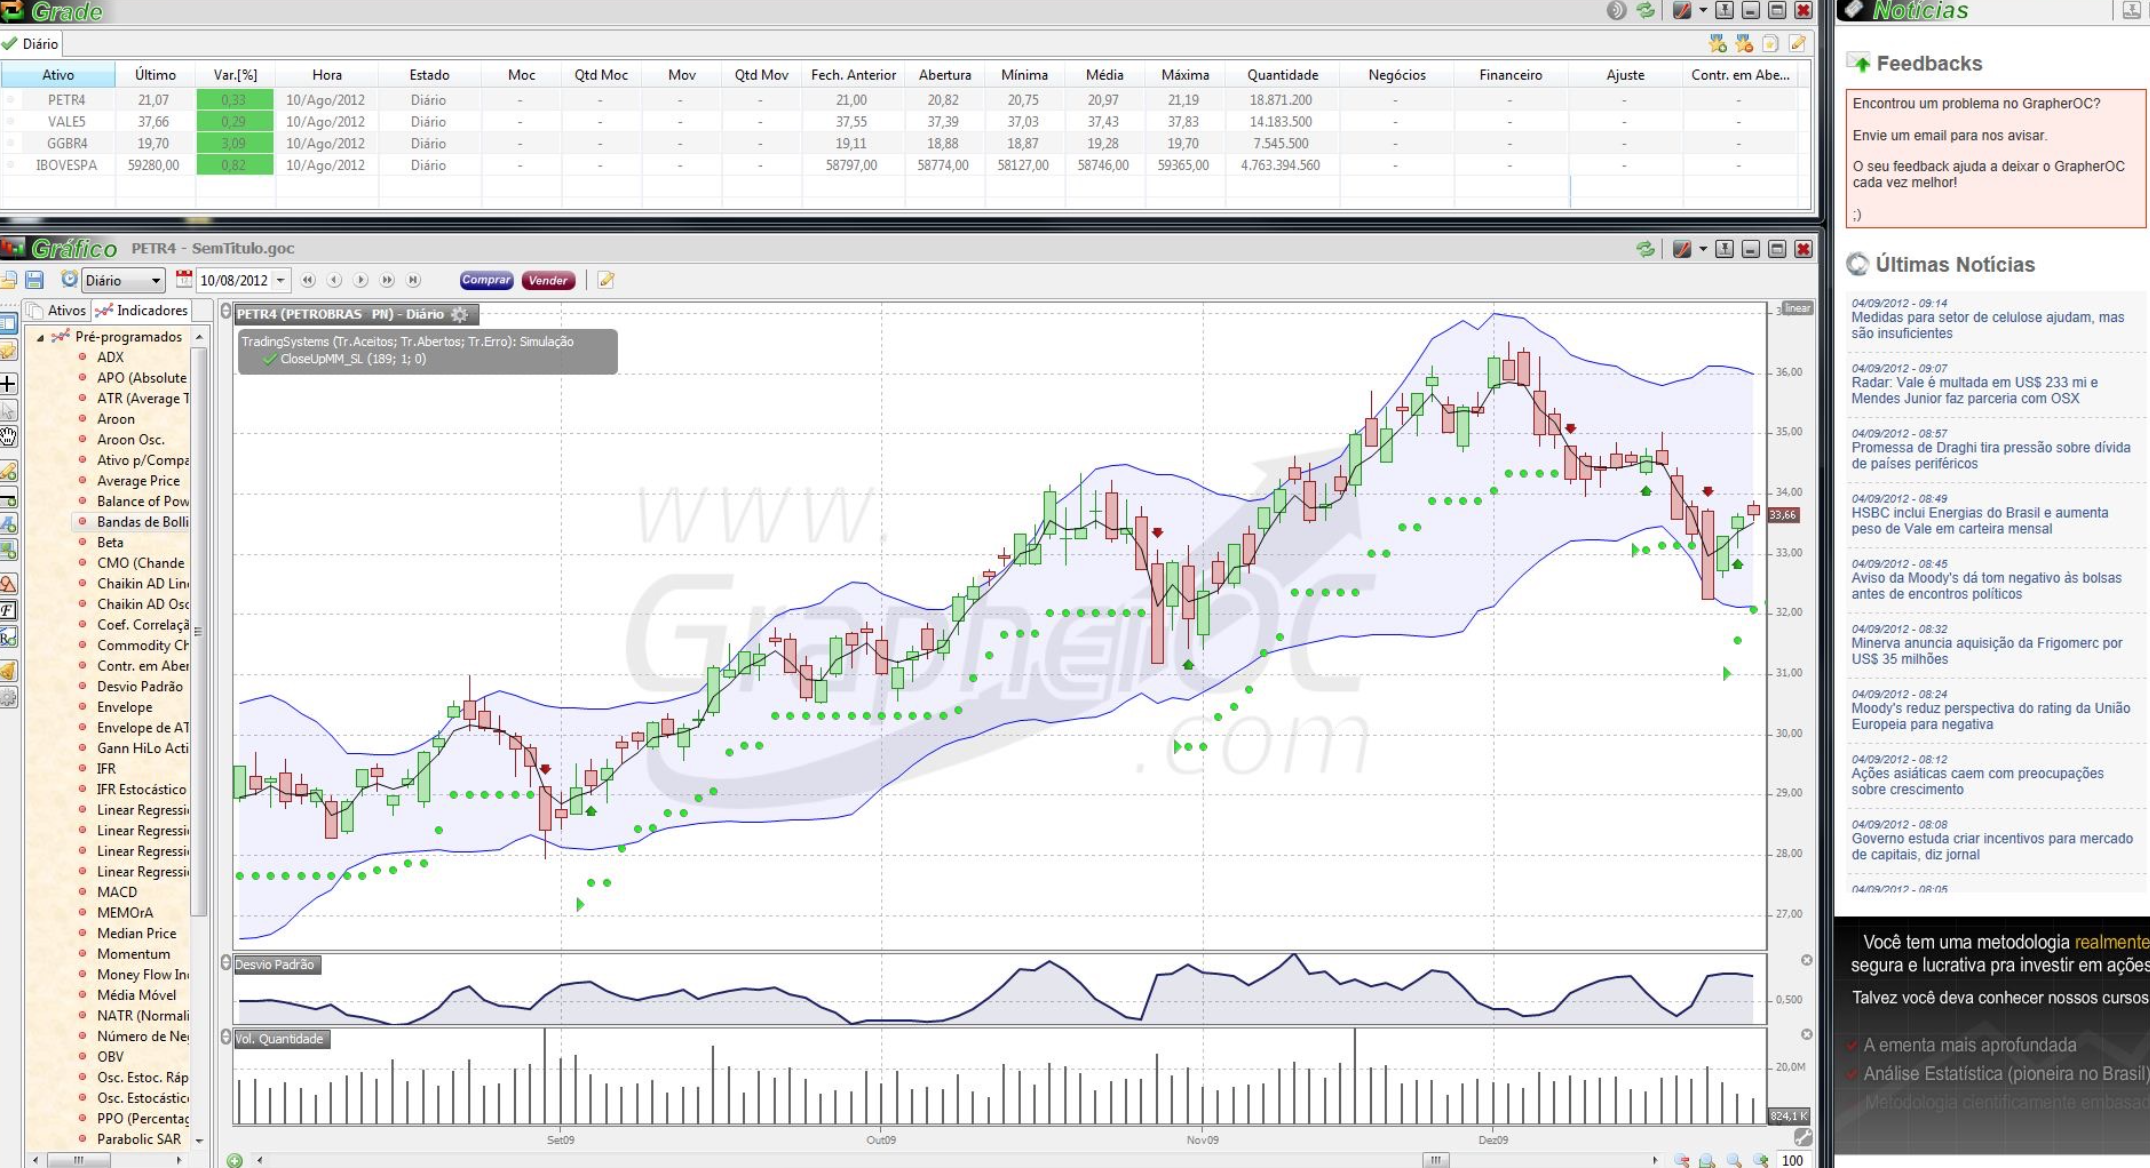
\includegraphics[width=0.5\textwidth]{figuras/f03}
\caption{GrapherOC}

\end{figure}

\subsubsection{Ferramentas de corretoras}

Corretoras de valores, como a XP Investimentos e Ágora, disponibilizam ao seus clientes ferramentas de envio de ordens de compra e venda (HomeBroker), bem como ferramentas de suporte para atividades de análise técnica. Porém, para usufruir o máximo possível delas, é requerido do usuário conhecimentos financeiros relacionados à análise técnica. No entanto, caso o cliente não tenha tais conhecimentos, as corretoras, normalmente, oferecem acompanhamento de profissionaiscapacitados para atuar no mercado.

\subsubsection{Meta Trader}

O MetaTrader (\ref{f04})é uma plataforma oferecida por corretoras estrangeiras. Essa ferramenta aborda o mercado de moedas (FOREX) e o de commodities, tais como petróleo. A plataforma possui um suporte tecnológico oferecido ao usuário, oferecendo ao mesmo uma IDE para desenvolver produtos de Software, conhecidos por robôs, em uma linguagem própria, Mql4. A linguagem Mql4 é uma linguagem estruturada, baseada na linguagem C,e sua evolução é o Mql5, a qual é uma linguagem orientada a objetos. No entanto, essa ferramenta requer do usuário conhecimentos relacionados ao Mercado Financeiro, além de conhecimentos de lógica de programação

\begin{figure}[h]
\centering
\label{f04}
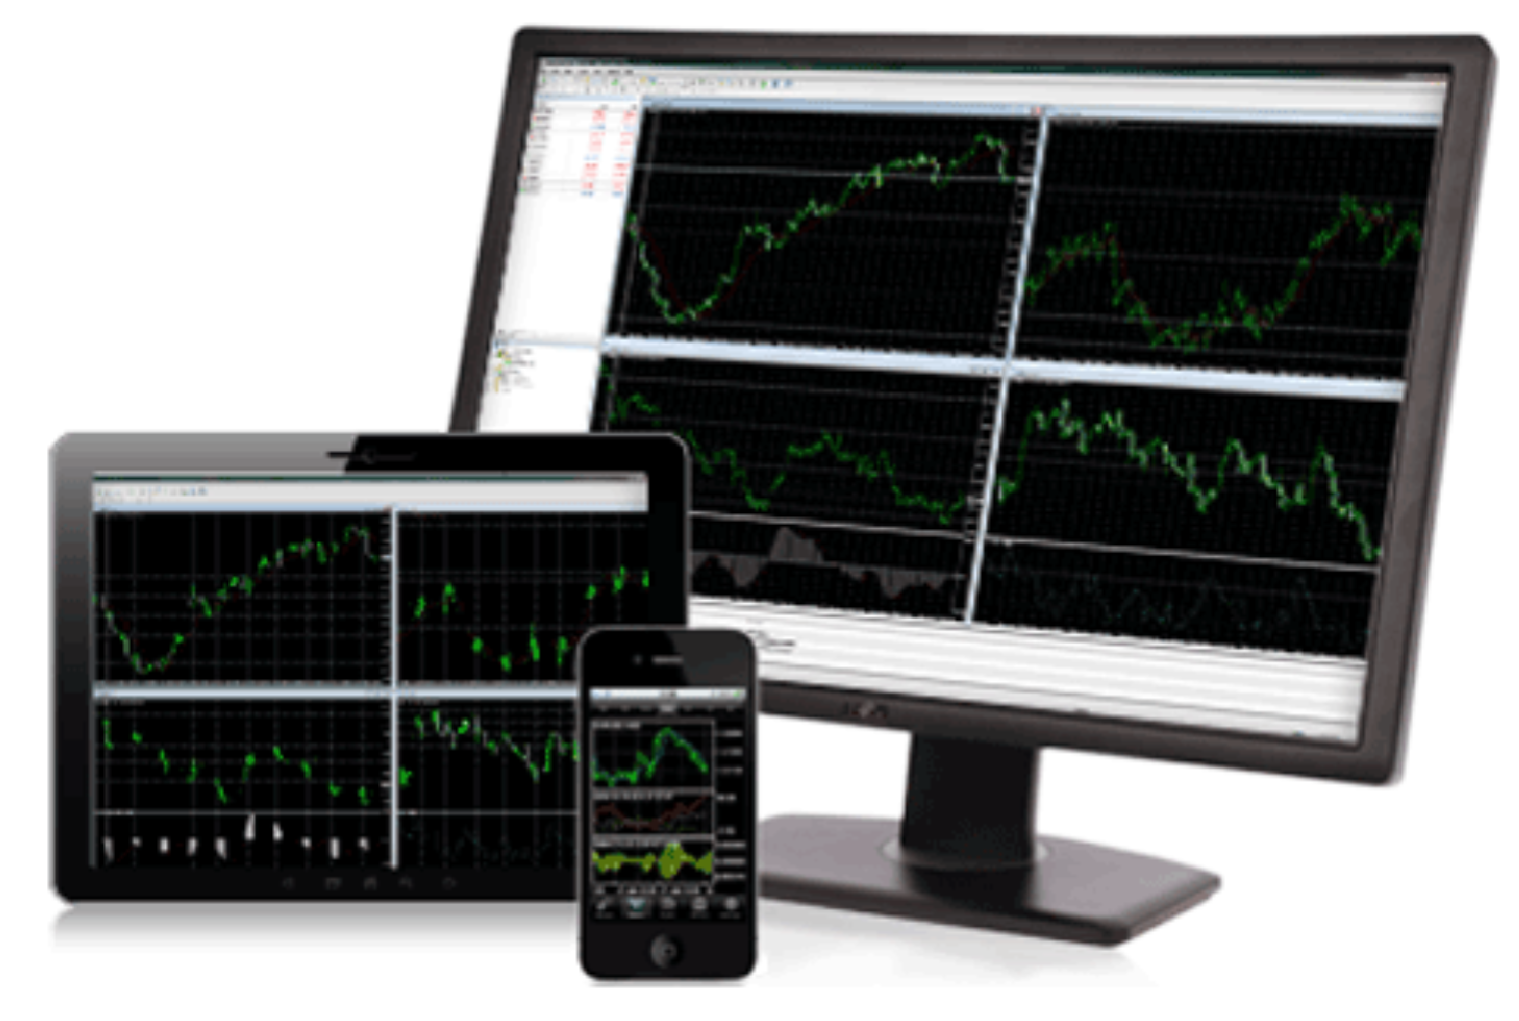
\includegraphics[width=0.5\textwidth]{figuras/f04}
\caption{MetaTrader}

\end{figure}


\subsubsection{Grafix}

O Grafix (\ref{f05}) é uma ferramenta somente para análise gráfica. Tornou-se Software livre no ano de 2012. Trata-se de um suporte construído em Java e seu desenvolvimento está estagnado, desde 2012, por falta de voluntários no desenvolvimento. Assim como as demais, essa ferramenta também exige de seus usuários conhecimentos relacionados a investimentos bem como se diferencia por não ser possível ao investidor enviar ordens de compra/venda diretamente por ela. Limita-se, portanto, apenas em possibilitar a análise do mercado de ações. No entanto, por ser um Software livre, esse suporte permite modificações, sendo possível incorporar novas funcionalidades.

\begin{figure}[h]
\centering
\label{f05}
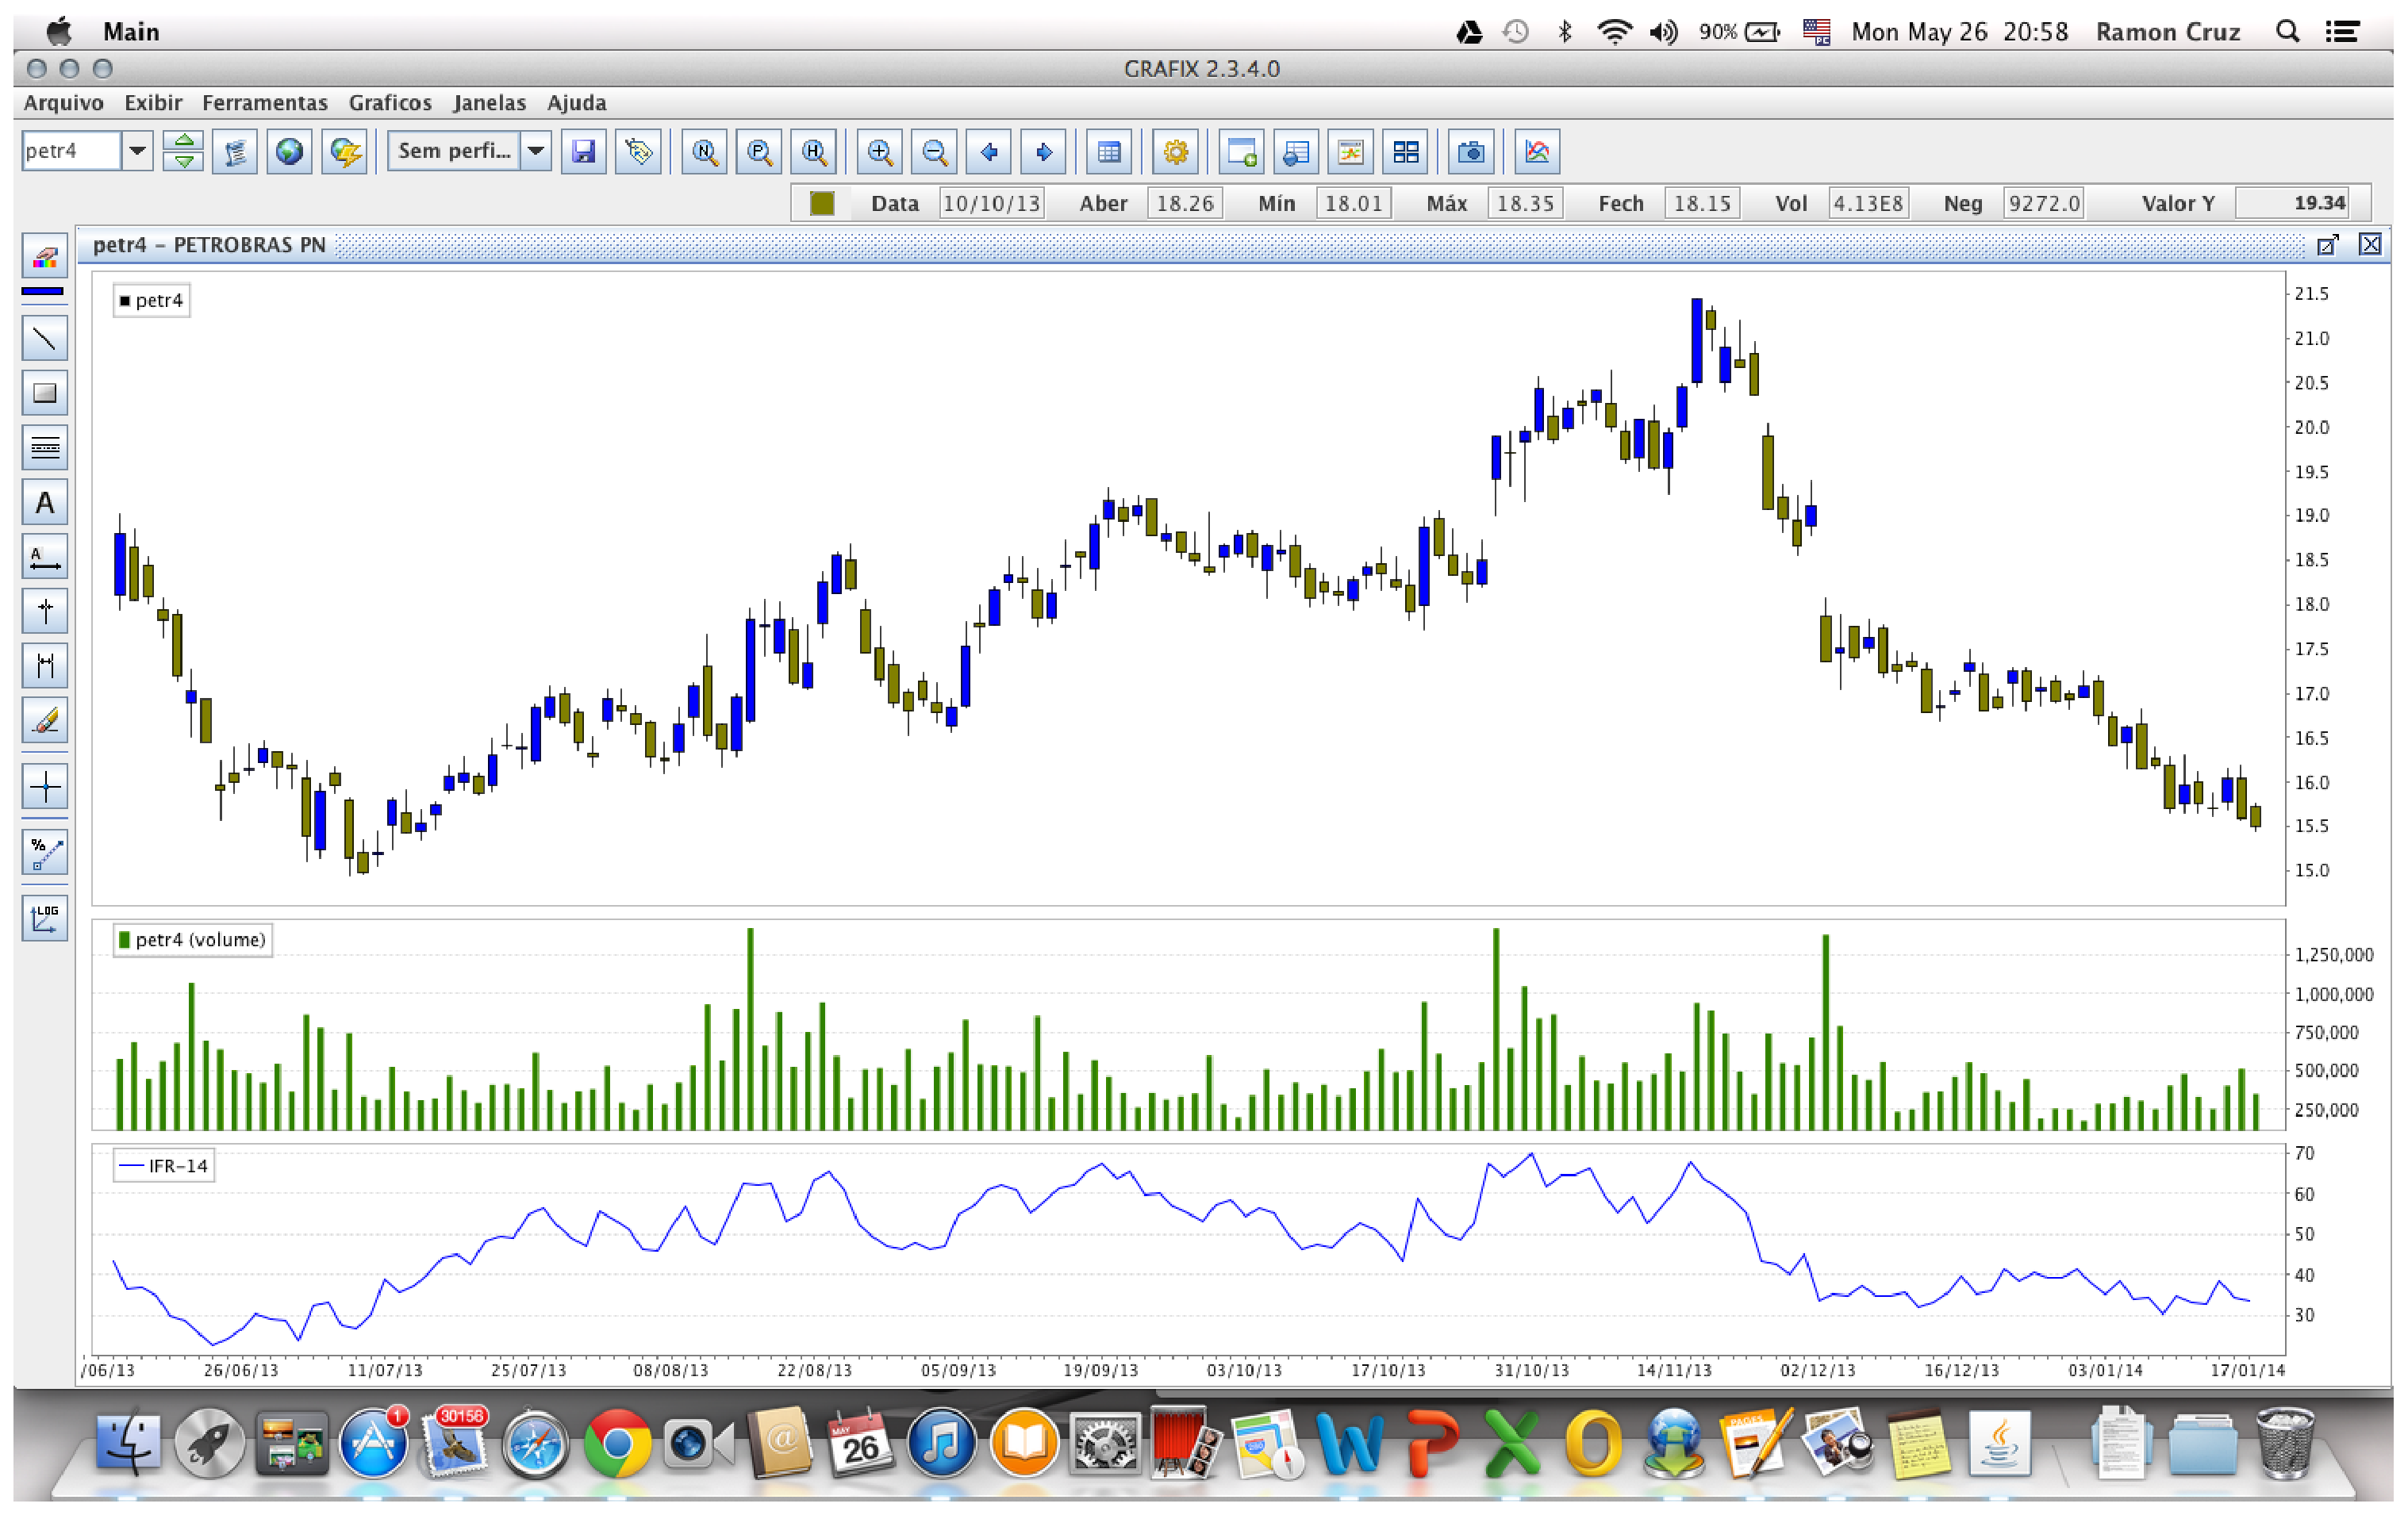
\includegraphics[width=0.5\textwidth]{figuras/f05}
\caption{Grafix}

\end{figure}

\section{ENGENHARIA DE SOFTWARE}
\subsection{Mode-View-Controller (MVC)}

Segundo Krasner e Pope (\citeyear{krasner1988}), quando construímos produtos de Software modularizando seus componentes, obtemos bons resultados. Isolar funcionalmente cada unidade permite aos desenvolvedores entenderem e modificarem mais facilmente cada unidade, sem que seja necessário conhecer todas as unidades envolvidas no Software em questão. Desta forma, uma arquitetura modularizada de um Software contribui para atividades de manutenção e evolução deste, tornando-as mais fáceis \cite[p. 1]{krasner1988}.


A arquitetura Model-View-Controller (MVC) concentra-se nos três módulos: (i) Model, éa representação o conhecimento que pode ser composto por um ou vários objetos;(ii) View, é a representação visual da Model, ou seja, é através daView que o usuário tem acesso às informações da Model; (iii)Controller, contém a interface entre a associação Models e Views com entradas de dispositivos (i.e. teclados, mouses, entre outros)\cite[p. 2]{krasner1988}.

Para manter todas Views e Controllers cientes das mudanças de estado ocorridas na Model, foi desenvolvida também a noção de dependência. Nesse contexto, os objetos do tipo Controller e View são registrados em uma lista de dependentes na Model, e quando ocorre alguma mudança, estes são avisados através de troca de mensagens \cite[p. 2]{krasner1988}, como ilustra a Figura 6(\ref{f06}). No \textit{capitulo 4, tópico 4.2.6} encontra-se uma explanação da aplicação do MVC na ferramenta proposta.

\begin{figure}[h]
\centering
\label{f06}
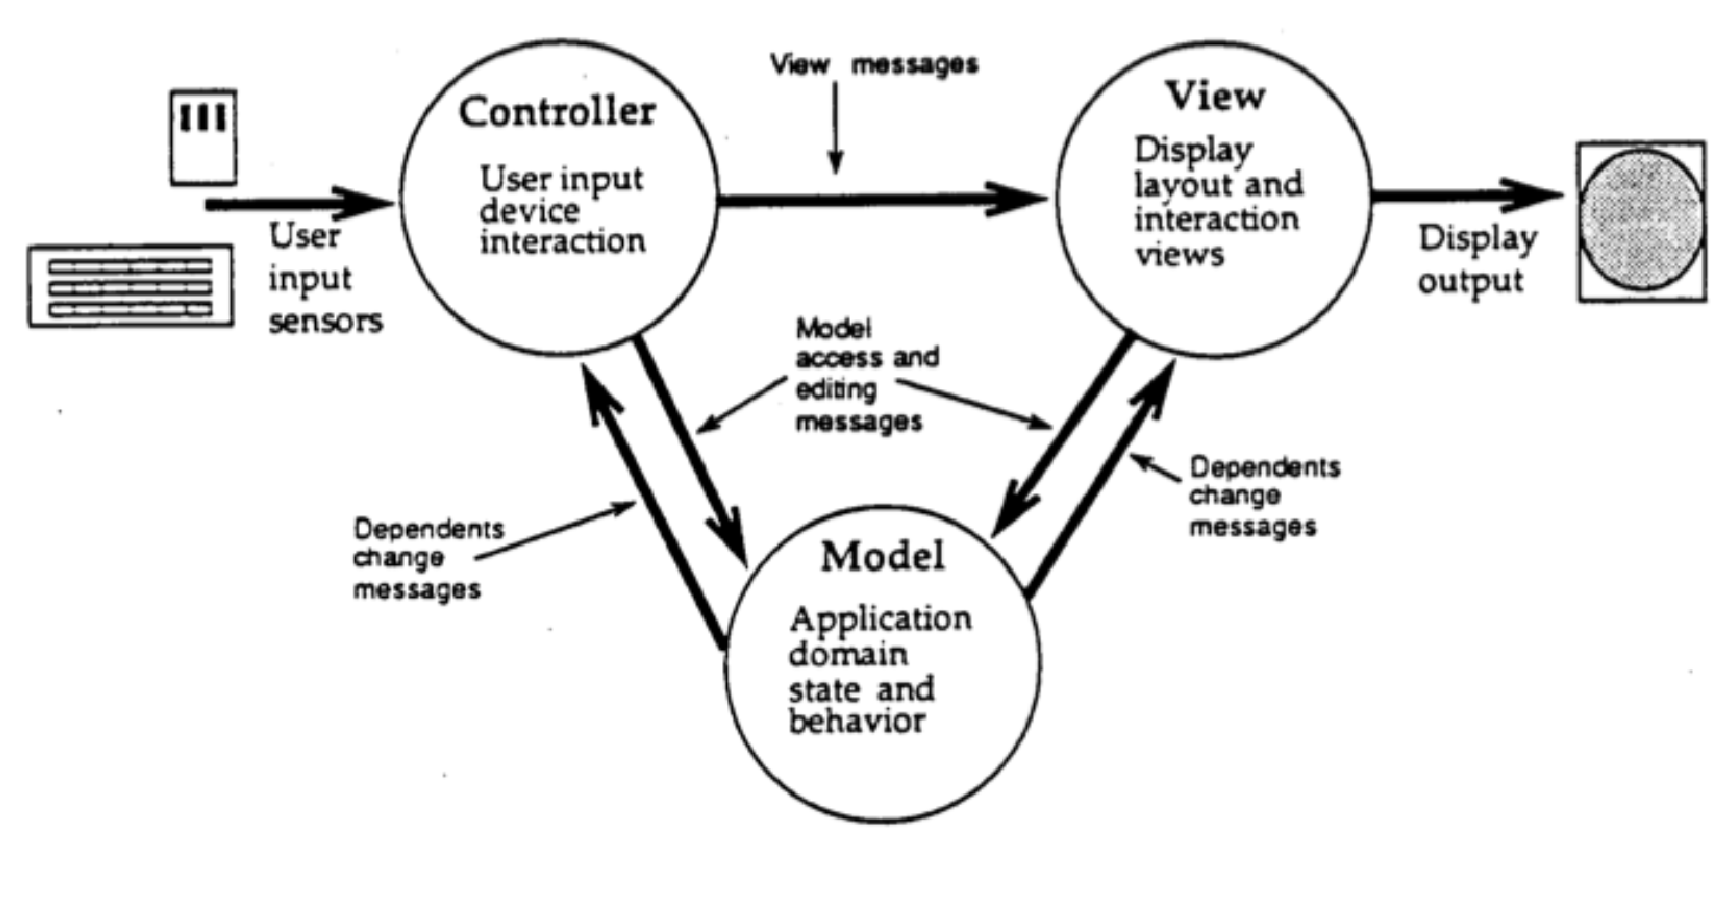
\includegraphics[width=1\textwidth]{figuras/f06}
\caption{Model-View-Controller e o envio de mensagens}

\end{figure}



\subsection{Padrões de Projeto}

Christopher Alexander afirma que \apud[p.19]{christopher1977}{gamma2000}, \textit{“cada padrão descreve um problema no nosso ambiente e o cerne da solução, de tal forma que você possa usar essa solução mais de um milhão de vezes, sem nunca fazê-lo da mesma maneira”}. Apesar do contexto de Alexander ser o da arquitetura, suas colocações aplicam-se no contexto de desenvolvimento de Software orientado a objetos. O núcleo de ambos tipos de projetos é a solução para um problema num determinado contexto \cite[p.19]{gamma2000}.

No contexto de Software, de acordo com Gamma (\citeyear{gamma2000},p.20): \textit{“Um padrão de projeto nomeia, abstrai e identifica os aspectos-chave de uma estrutura de projeto comum para torná-la útil para criação de um projeto orientado a objetos reutilizável”}. Cada padrão de projeto tem como objetivo solucionar um problema em particular. Para Gamma, um padrão de projeto tem quatro elementos essenciais: (i) Nome do padrão, descreve o problema em uma ou duas palavras; (ii) Problema, descreve a aplicação do projeto; (iii) Solução, descreve os elementos que compõe um projeto, seus relacionamentos, responsabilidades e colaborações; (iv) Consequências, descreve as vantagens e desvantagens de cada padrão \cite[p.19]{gamma2000}.

\subsubsection{Padrões de projeto adotado neste TCC}

\subsubsubsection{Strategy}

Trata-se de um padrão comportamental, o qualpermite a variação de algoritmos, independentemente dos clientes que os usam, facilitando ainda ser sensível ao contexto. OStrategy é composto por três participantes: (i) Context, é quem chama uma estratégia através de uma entidade do tipo interface; (ii) Strategy, é a interface comum a todos os algoritmos relacionados à ela; e (iii) ConcreteStrategy, é a classe concreta que implementa os diferentes algoritmos \cite[p.294]{gamma2000}. 

Como o padrãoStrategy delega a implementação de algoritmos às classes concretas bem como se baseia na implementação usando entidades do tipo interface,esse padrão oferece maior facilidade na manutenção de Software, em especial na manutenção evolutiva do mesmo. A Figura 7 (\ref{f07}) ilustra a arquitetura básica deste padrão \cite[p.295]{gamma2000}. Durante o desenvolvimento da ferramenta proposta, outros padrões de projetos poderão ser adotados, conforme a necessidade.

\begin{figure}[h]
\centering
\label{f07}
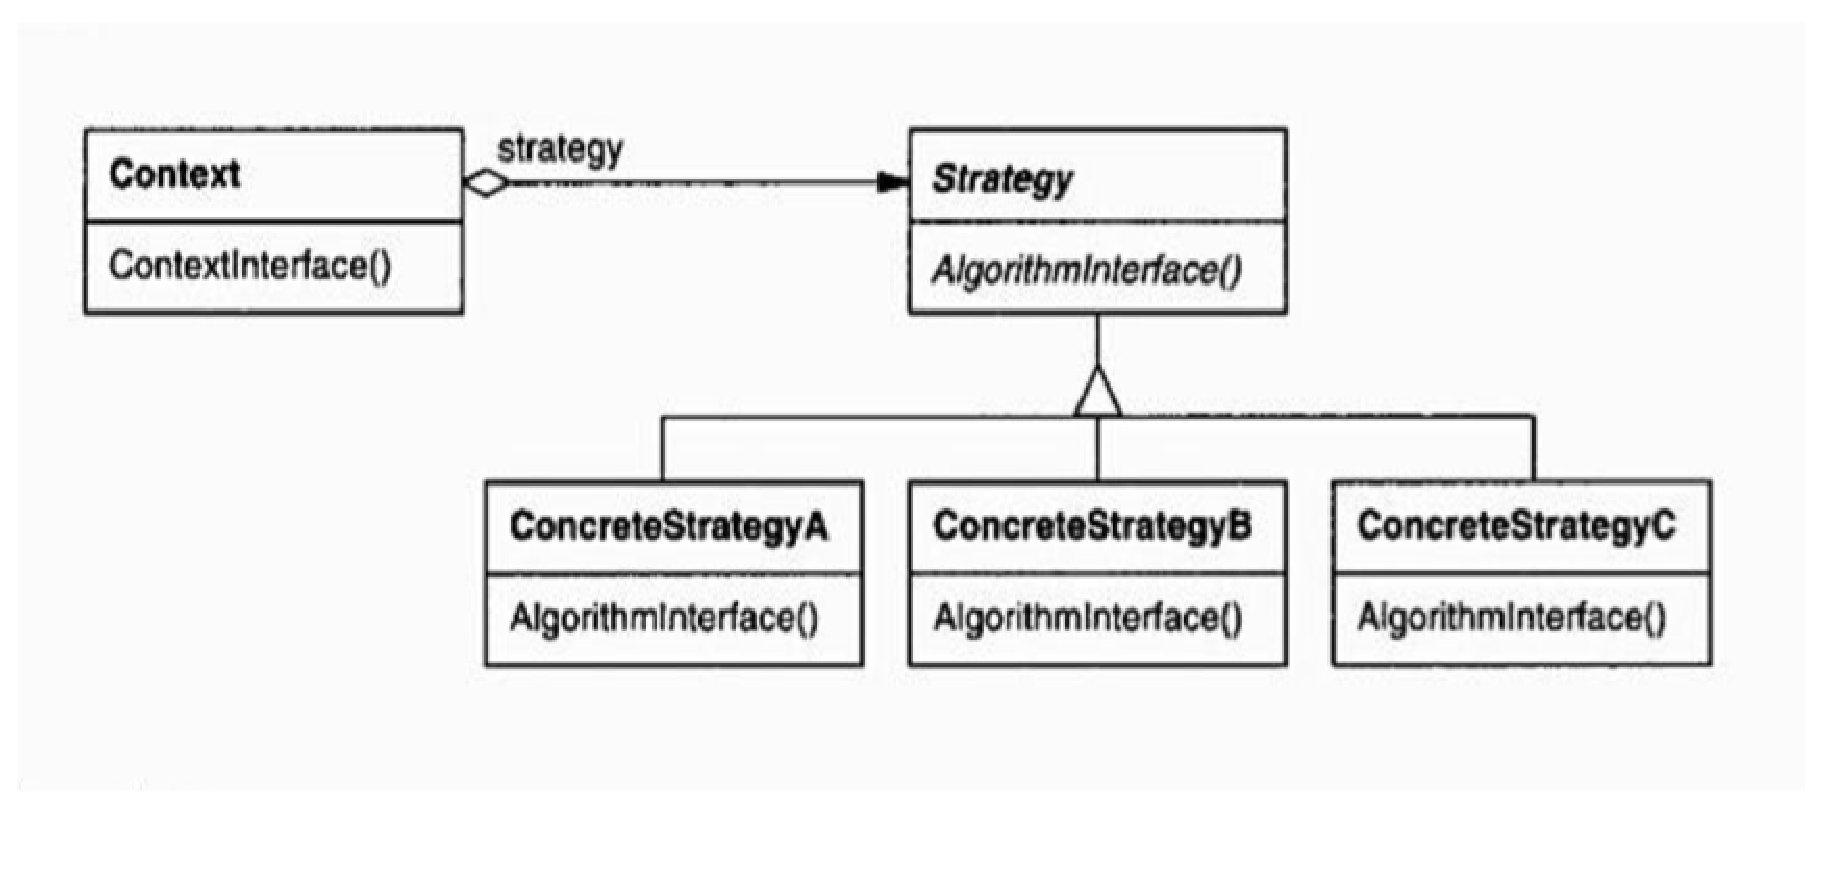
\includegraphics[width=0.9\textwidth]{figuras/f07}
\caption{Padrão Strategy}

\end{figure}

\subsection{JADE (Java Agent Development Framework)}

O JADE \cite{telecon2014} é um framework implementado em Java que possibilita a implementação de Sistemas Multiagentes complexos. O JADE oferece suporte para testes de atividade de debug, arquitetura bem estabelecida para criação, comunicação, identificação, gerenciamento e demais ações com vários agentes atuando como em uma sociedade real. No JADE, os agentes podem trocar mensagens entre si, caracterizando sua arquitetura de comunicação como troca de mensagem (arquitetura descrita brevemente no tópico \textbf{2.2.1.2}). Este framework foi desenvolvido de acordo com as especificações Foundation for IntelligentPhysicalAgents (FIPA) \cite{telecon2014}, que é uma comunidade IEEE que promove padrões tecnológicos para Sistemas Multiagentes. Por ter sido implementado integralmente em Java, o JADE pode ser executado em qualquer sistema operacional que possua uma Máquina Virtual Java.

O JADE é um Software livre e distribuído pela Telecom Itália, empresa proprietária da TIM Brasil, e possui a Licença LGPL \cite{telecon2014}. Ele é supervisionado por um grupo de empresas de cinco membros: Telecom Itália, Motorola, Whitestein Technologies AG, ProfactorGmbH e France Telecom R\&D. Atualmente, a versão disponível é a 4.3.2, publicada em 28 de março de 2014.

\begin{figure}[h]
\centering
\label{f08}
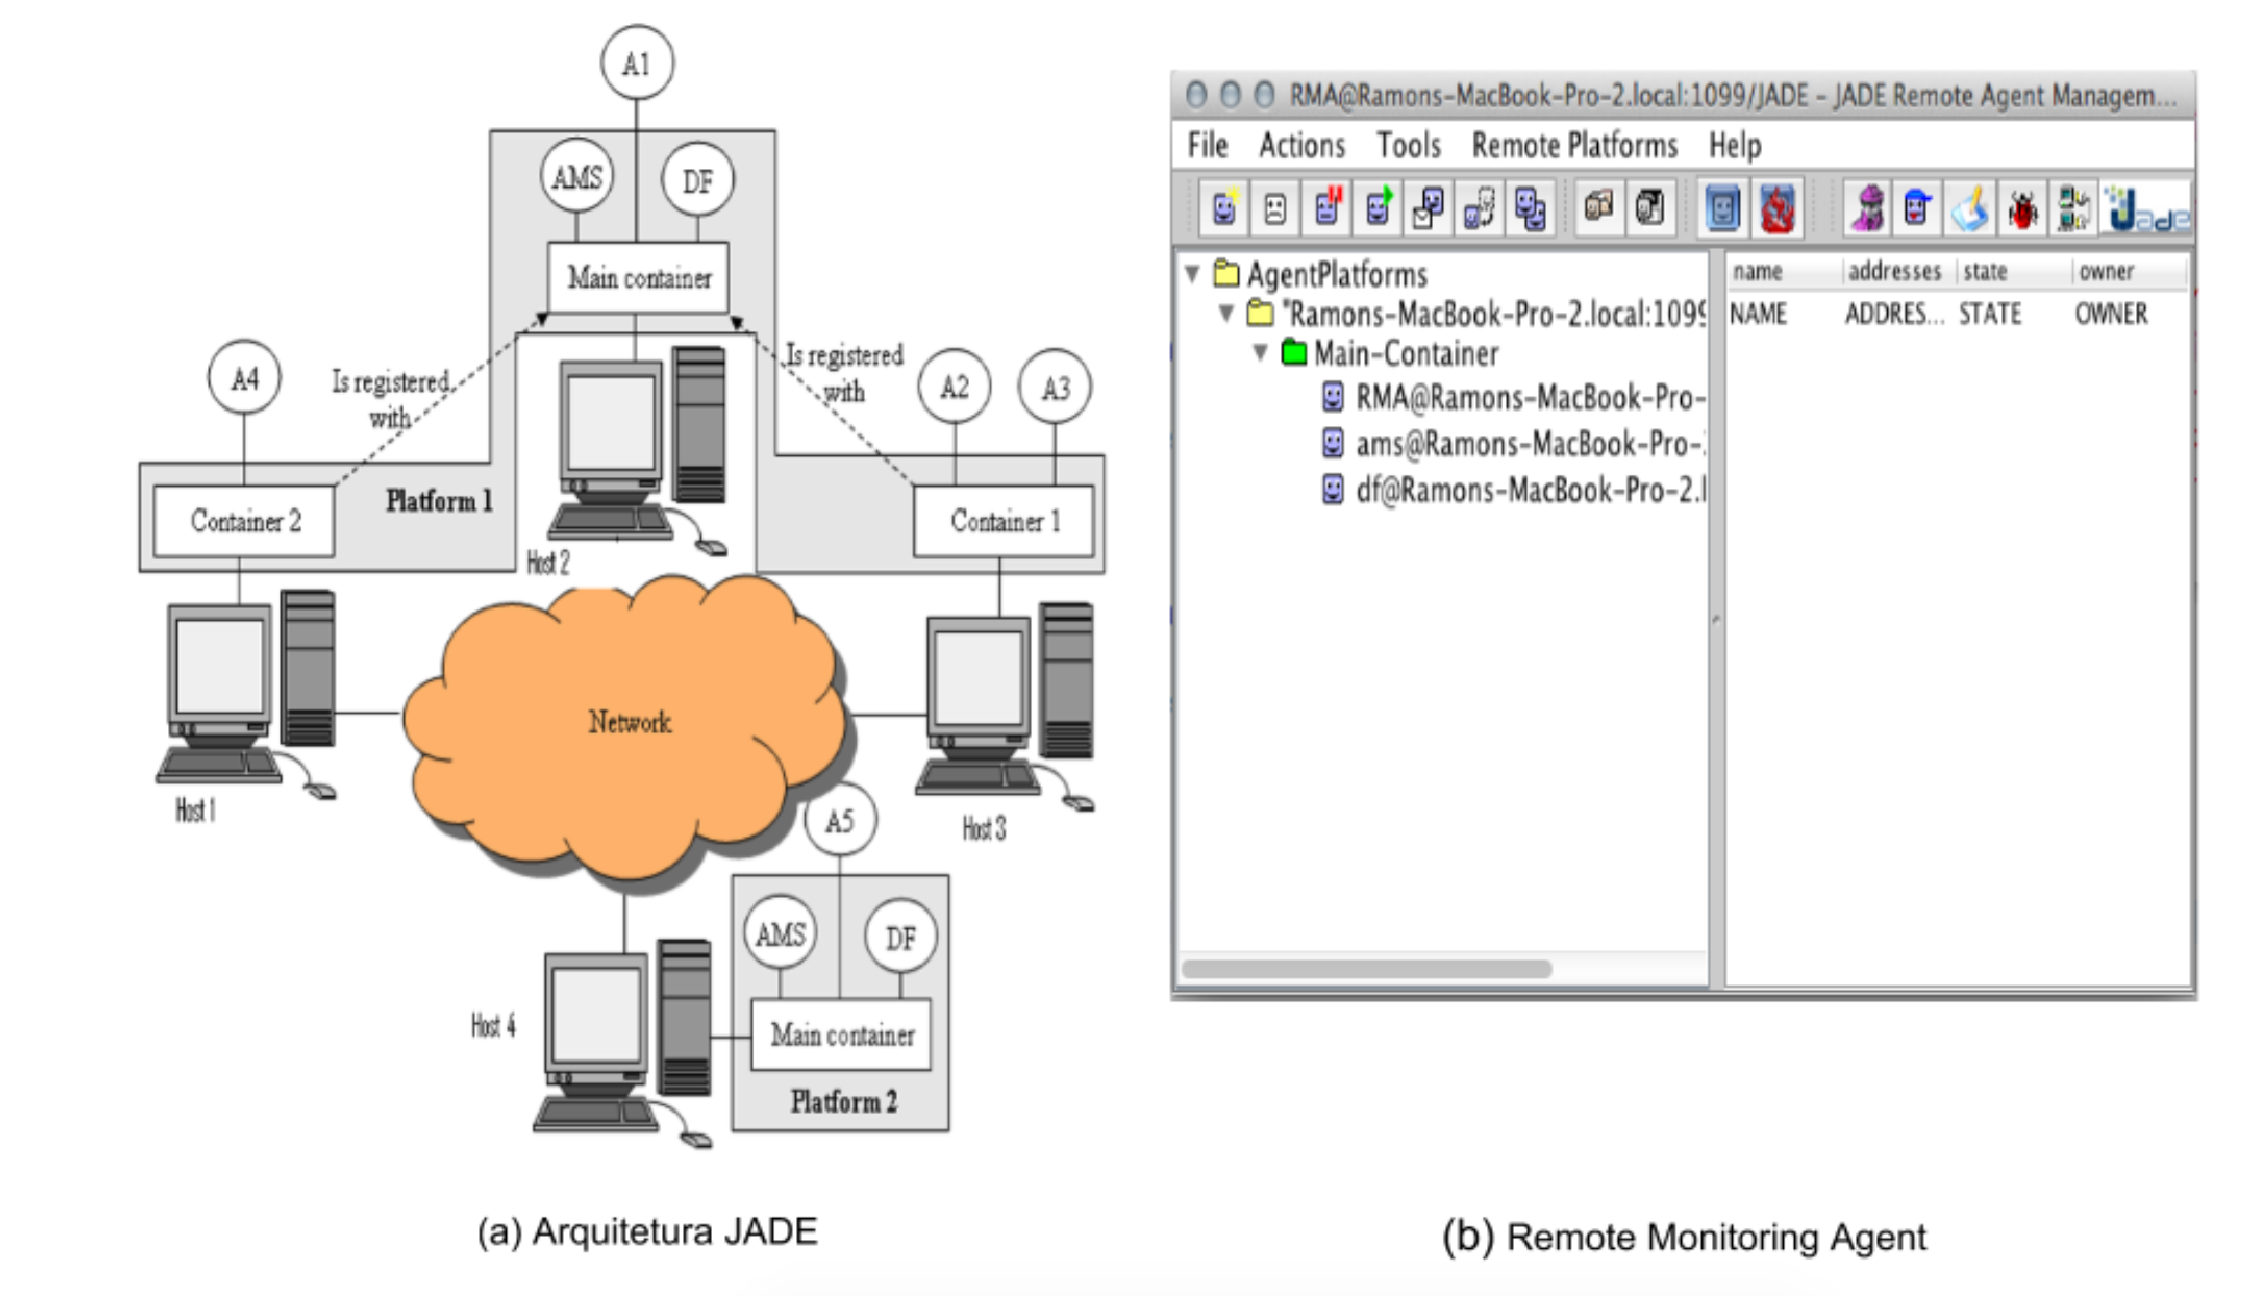
\includegraphics[width=0.9\textwidth]{figuras/f08}
\caption{Arquitetura JADE}

\end{figure}


Considerando a Arquitetura da Plataforma JADE apresentada na Figura 8.a(\ref{f08}), cada Agente instanciado fica contido em um Container, sendo que este pode ter um ou vários agentes. Existem dois tipos de containers, o main e o padrão. O main container contém, por padrão, três agentes: (i) Agente DF (DirectoryFacilitator), agente responsável por prover serviços, conhecidos no JADE como páginas amarelas, nos quais um dado agente pode encontrar outros agentes, iniciar comunicação com terceiros e registrar/cadastrar os serviços que presta a terceiros; (ii) Agente AMS (Agent Management System), agente responsável por prover serviços de páginas brancas, sendo capaz de criar e excluir agentes em containers remotos ou locais, gerenciando o ciclo de vida dos agentes na plataforma como um todo; e (iii) Agente RMA (Remote Monitoring Agent) (Figura 8.b(\ref{f08})), agente responsável por gerenciar as consoles gráficas providas pela Plataforma JADE.

Simplificadamente, na Arquitetura do JADE, uma dada plataforma é composta por um ou vários containers, estes containers podem estar em um computador ou distribuídos em uma rede de computadores, como ilustrado na Figura 8a(\ref{f08}). A arquitetura JADE possibilita ainda a comunicação entre os agentes independentemente do container onde estes se encontram, ou seja, o agente A2 pode se comunicar com o agente A3, assim como pode se comunicar também com o agente A5, o qual está em outro container, em outra plataforma, porém conectado a uma rede de computadores. Adicionalmente, serviços, conteúdos e servidores podem ser compartilhados usando como base essa rede de computadores, permitindo aos agentes trabalharem de forma colaborativa, conquistando objetivos até mesmo não triviais, centrados no princípio Dividindo para Conquistar. Princípio esse oriundo de contextos político-sociais bem como amplamente utilizado na atualidade, na ciência da computação como um todo, como uma técnica capaz de lidar com problemas complexos, dividindo esse problema em instâncias menores, resolvendo essas instâncias isoladamente e agrupando os resultados para atingir uma conquista maior, ou seja, a solução do problema de maior complexidade.


\subsection{Metodologia Scrum}

O termo Scrum  é originário do Rugby, esporte criadona Inglaterra. No Scrum, são feitas entregas contínuas de pequenas partes funcionais do Software. O Scrum consiste em times associados a papéis, eventos, artefatos e regras. Cada componente tem uma função específica no desenvolvimento do Software \cite{schwaber2013}.

O time Scrum é formado por:(i)um Scrum Master, que é a figura do líder do time. Ele é o responsável por fazer o time compreender as regras do Scrum; (ii)um grupo de desenvolvimento (time), que são os programadores, designers, entre outros; e (iii) umProductOwner, que é uma pessoa com bom conhecimento das necessidades do produto. No Scrum, os times são auto-organizáveis no que tange à escolha da melhor forma para realizar um trabalho. O modelo de time no Scrum foi pensado de forma que valorize a flexibilidade, criatividade e produtividade.  O time entrega produtos de forma iterativa e incremental, assim aumentando oportunidades de feedback contínuo. Estas entregas são versões parciais funcionais do Software trabalhado pelo time \cite[p. 5-7]{schwaber2013}.

Cada evento no Scrum é uma oportunidade de verificar e corrigir algo no produto. Eles são projetados para que seja possível obter transparência e uma inspeção criteriosa do produto. Cada evento termina sempre que seu objetivo é alcançado. No Scrum, o evento principal é a Sprint. Ela é o ciclo de desenvolvimento do produto, que dura um mês ou menos, sendo composta por:(i) uma reunião de planejamento; (ii) reuniões diárias curtas; (iii) uma revisão daSprint, (iv) uma retrospectiva; e o  (v) trabalho de desenvolvimento do produto.

Segundo Schwaber e Sutherland (\citeyear{schwaber2013}, p.13), \textit{“Os artefatos do Scrum representam o trabalho ou o valor para o fornecimento de transparência e oportunidade para inspeção e adaptação.”} Os artefatos são elaborados de forma que o entendimento das informações contidas nele seja o maior possível. Dentre os artefatos do Scrum temos: (i) Backlog do Produto, é uma lista de tudo que é necessário no produto. Ela é a origem dos requisitos e é gerida pelo ProductOwner. O Backlog do Produto é dinâmico e existe enquanto houver o produto; (ii) Backlog da Sprint, é o conjunto de itens selecionados do Backlog do Produto para a Sprint, ou seja, é o conjunto de características que serão implementadas pelo time durante a Sprint; (iii) Incremento, é a soma de todas os itens do Backlog do produto entregues no final de uma Sprint \cite[p. 13-15]{schwaber2013}. A aplicação adaptada desta metodologia encontra-se no \textbf{capitulo 5, tópico 5.2.}


\section{RESUMO DO CAPÍTULO}

Elucidou-se nesse capítulo, no Contexto Financeiro, uma breve exposição de algumas ferramentas de análise técnica comumente encontradas no Mercado Financeiro para apoiar o investidor. Destaca-se nelas uma característica em comum, que é a necessidade de seu usuário possuir conhecimentos relacionados à análise técnica. 

Na Engenharia de Software, foi apresentado um modelo arquitetural bastante aceito, o Model-View-Controller. Este modelo concentra-se na divisão da arquitetura de um Software em três módulos autônomos que se comunicam entre si. Foi apresentado ainda o padrão de projeto Strategy, que será adotado neste TCC. 

Adicionalmente, foi descrito o framework JADE, o qual é adotado neste TCC para implementar os agentes comportamentais planejados para o desenvolvimento da ferramenta proposta. E por fim, foi apresentada a metodologia Ágil, que será adaptada para conduzir o desenvolvimento da ferramenta proposta por este TCC.

\newpage
\chapter[PROPOSTA]{PROPOSTA}
\section{PROCESSO INVESTIGATIVO}
Nesta etapa do TCC, foi elaborado um cenário para avaliar o esforço necessário do autor para implementar um Software nas linguagens Java, Mql4 e Python. Para isso, foram adotadas as seguintes etapas para realizar uma prova de conceito: (i) Elaborar cenário, onde foi eleito um padrão de formação encontrado nos gráficos de candlesticks e foi elaborada uma hipótese inicial; (ii) Selecionar  ativos, onde foram eleitas algumas ações com seus devidos valores históricos para testar os produtos de  Software; (iv) Implementar, onde os algoritmos foram implementados nas três linguagens escolhidas; (v) Analisar resultados, onde foi feita a análise manual dos resultados afim de verificar o grau de acerto. Estas etapas estão descritas nos subtópicos seguintes e ilustrado na Figura 9(\ref{f09}).


\begin{figure}[h]
\centering
\label{f09}
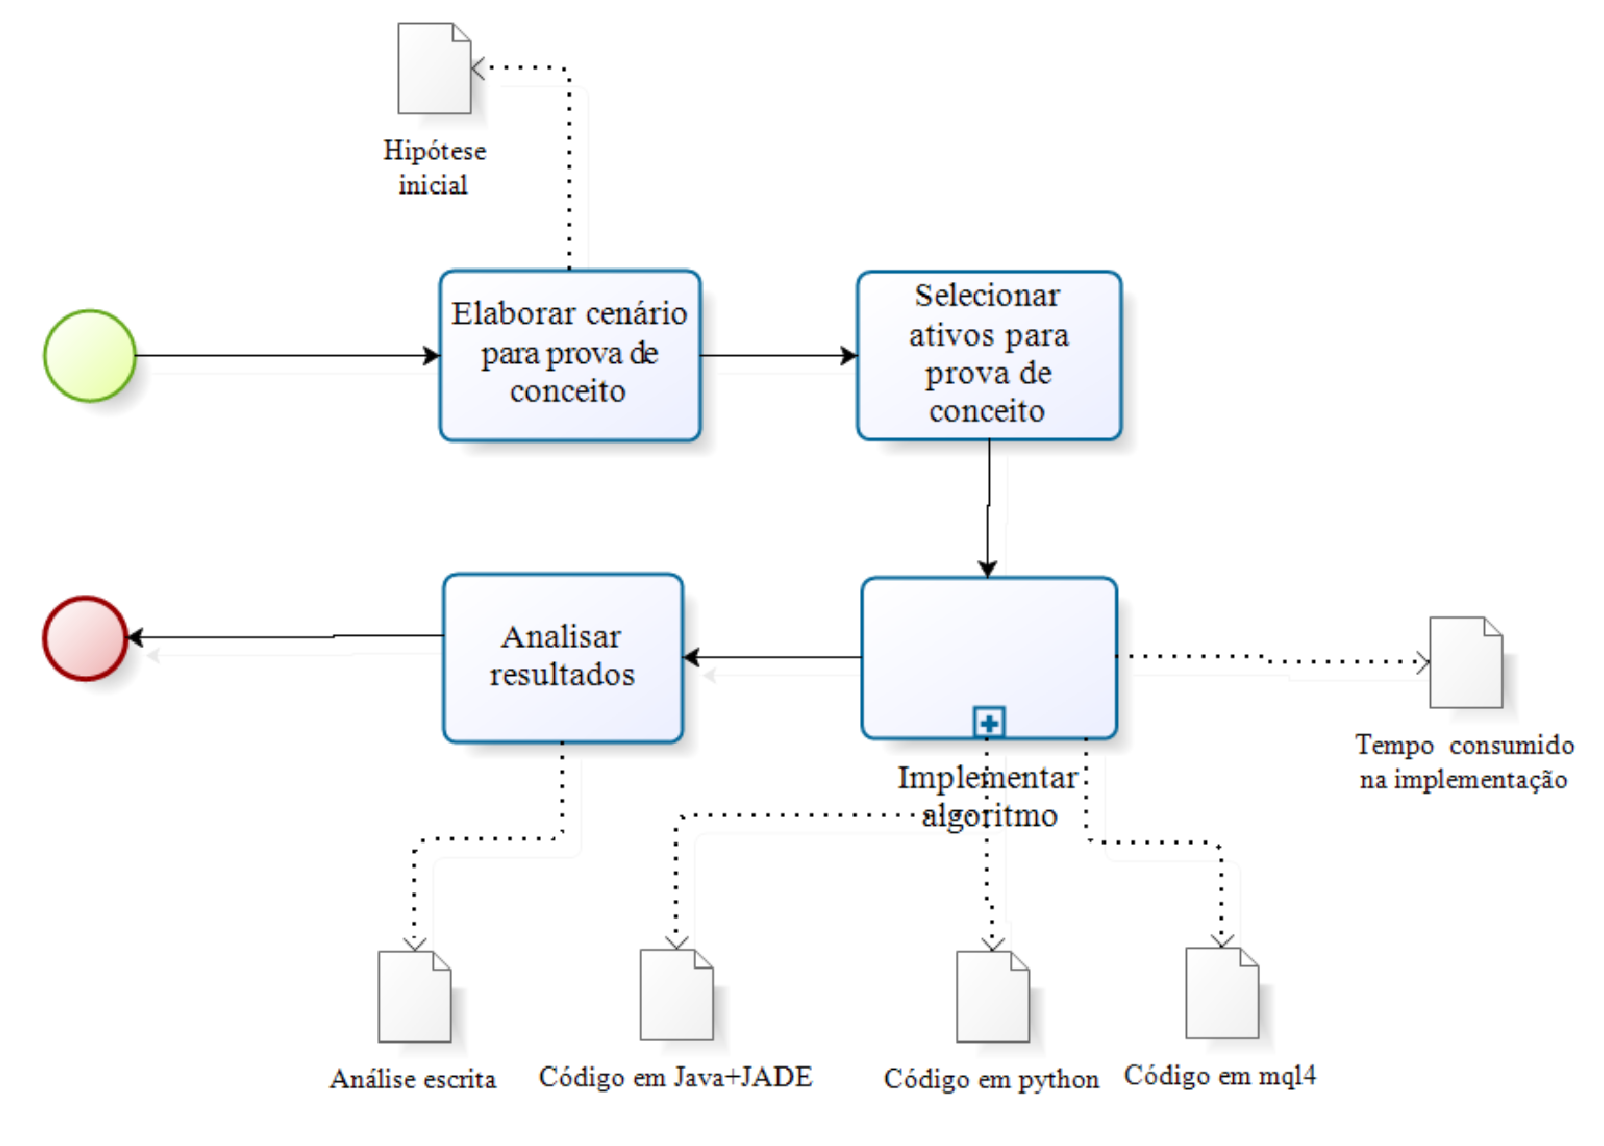
\includegraphics[width=0.9\textwidth]{figuras/f09}
\caption{Processo investigativo }

\end{figure}
\subsection{Processo investigativo}

Para nortear as provas de conceitos feitas para este estudo, foi elaborado um cenário onde é requerido uma maneira automatizada de se chegar à uma solução. Este cenário é descrito a seguir.

\begin{adjustwidth}{1,5cm}{0cm}
\textit{Uma das maneiras de um investidor acompanhar as movimentações do mercado de capitais, mais especificamente uma Bolsa de Valores, é através de gráficos como: (i) o gráfico de barras ; (ii) o gráfico de linha  e (iii) o gráfico de candlestick\cite[p. 5-6]{matsura2006}. Considerando o último, deseja-se encontrar uma maneira automatizada bem como a formação do padrão de candlestickconhecido como Dark cloud \cite[p.61]{matsura2006}. Padrão este, que poderá compor um plano estratégico de investimento.}

\textit{Uma candlestick é formada por 4 valores: (i) valor de abertura; (ii) valor de máxima; (iii) valor de mínima; e (iv) valor de fechamento. Quando o valor de  fechamento é maior do que o valor de abertura tem-se uma candlestick de alta, quando ocorre o inverso tem-se uma candlestick de baixa. A Figura 10(\ref{f10}) ilustra uma candlestick de alta, que é representada com o preenchimento em branco e umacandlestick de baixa, que é representada com o preenchimento em vermelho. Cada candlestick representa uma periodicidade, a qual pode ser desde um minuto até um ano \cite[p.6]{matsura2006}.}
\end{adjustwidth}

\begin{figure}[h]
\centering
\label{f10}
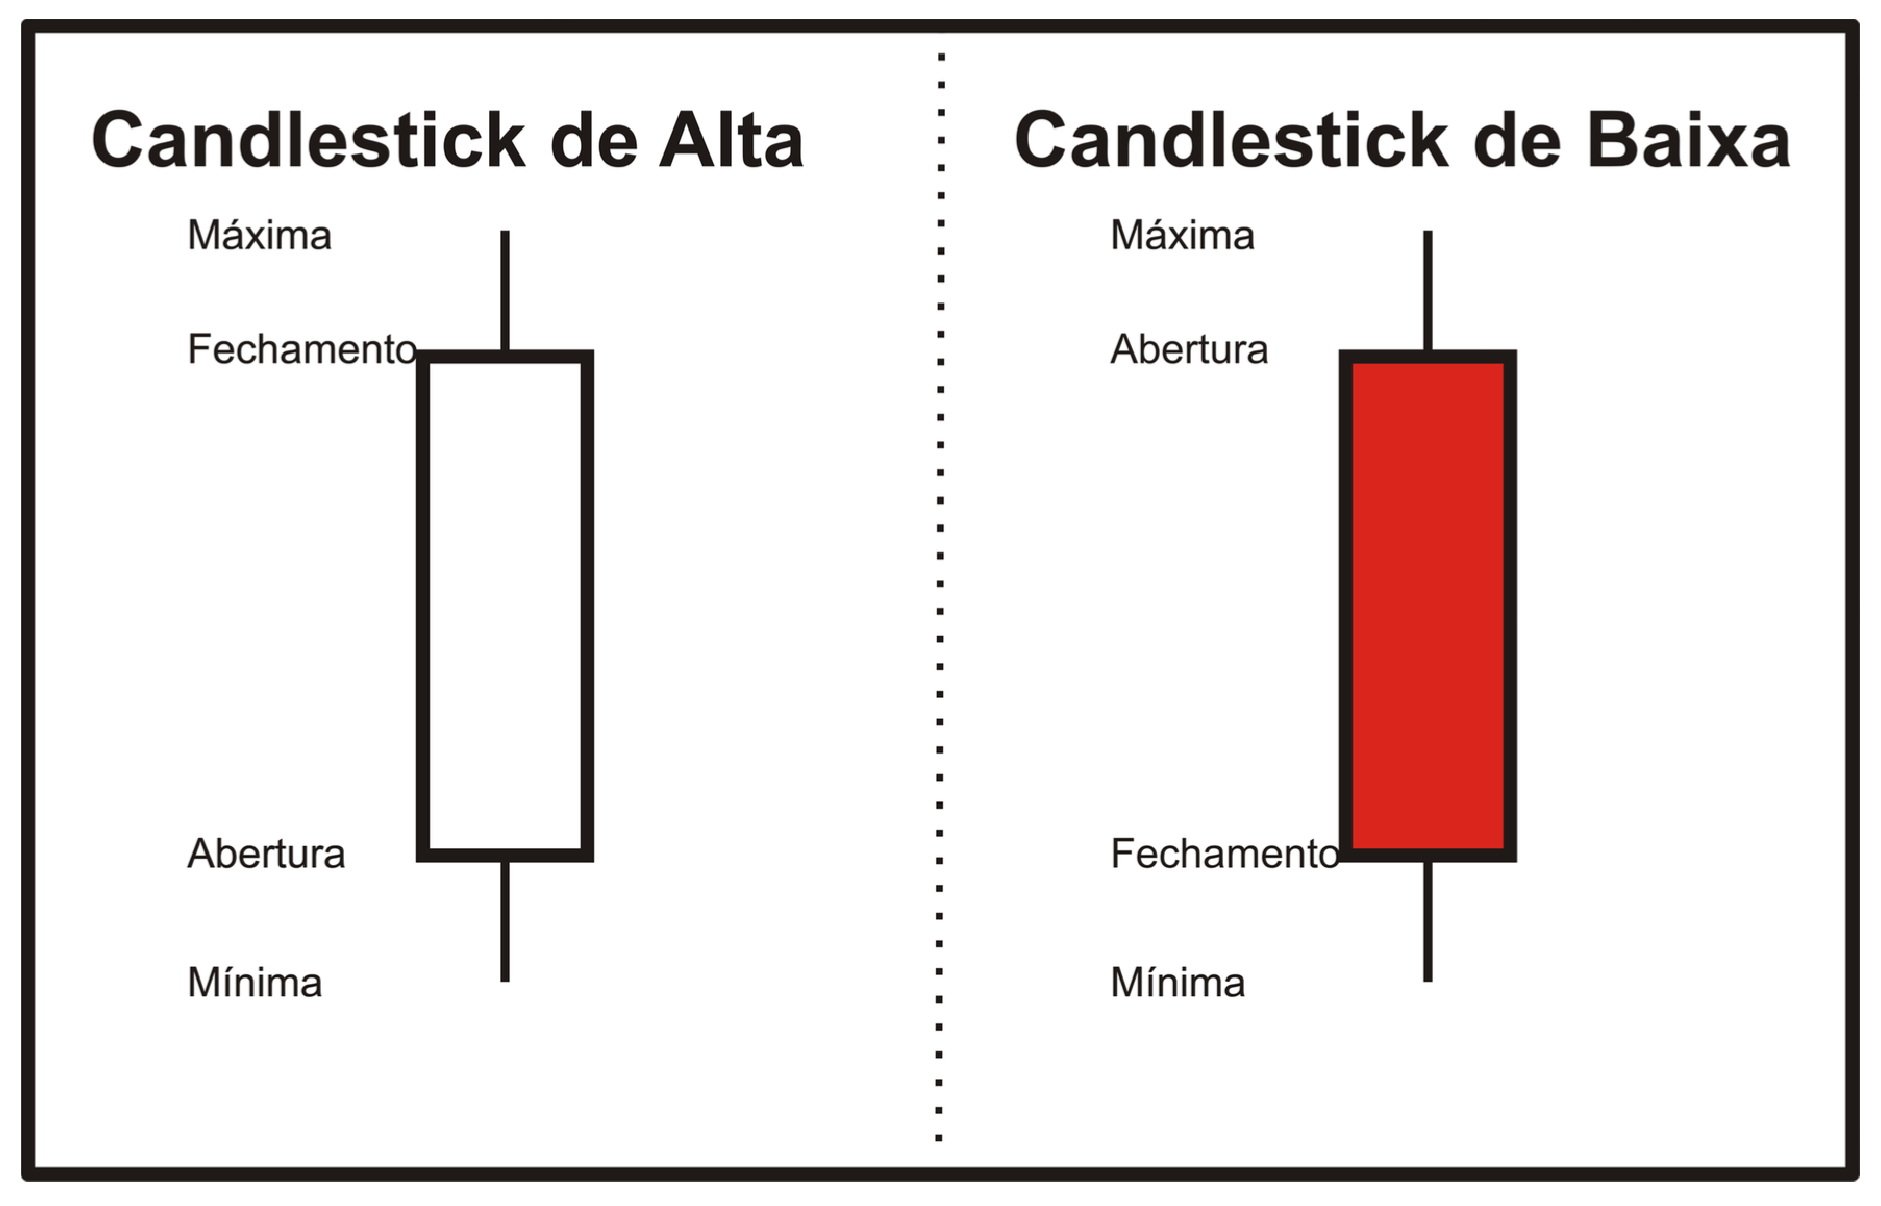
\includegraphics[width=0.8\textwidth]{figuras/f10}
\caption{Candlestick }

\end{figure}

O padrão Darkcloud (Figura 11[\ref{f11}]) é formado por duas clandlesticks, sendo a primeira de alta e a segunda de baixa, onde a segunda tem a abertura maior que a máxima da primeira e fechamento maior que a abertura da primeira \cite[p.61]{matsura2006}.Bigalow faz a seguinte interpretação deste padrão.

\begin{citacao}
Após uma forte tendência de alta, a atmosfera está altista. O otimismo está presente. O preço abre com gap para cima. Os vendedores aparecem e empurram os preços de volta para baixo. Finalmente, o preço fecha na ou próximo das mínimas do dia. O fechamento não confirmou a maioria dos ganhos do dia anterior. Os comprados agora estão preocupados. Obviamente observam que a tendência de alta deve se encerrada. Este sinal proporciona uma boa venda a descoberto, com um estope acima da máxima do dia da vela preta (candlestick de baixa) . \newline \cite[p.47]{bigalow2010}

\end{citacao}
\begin{figure}[h]
\centering
\label{f11}
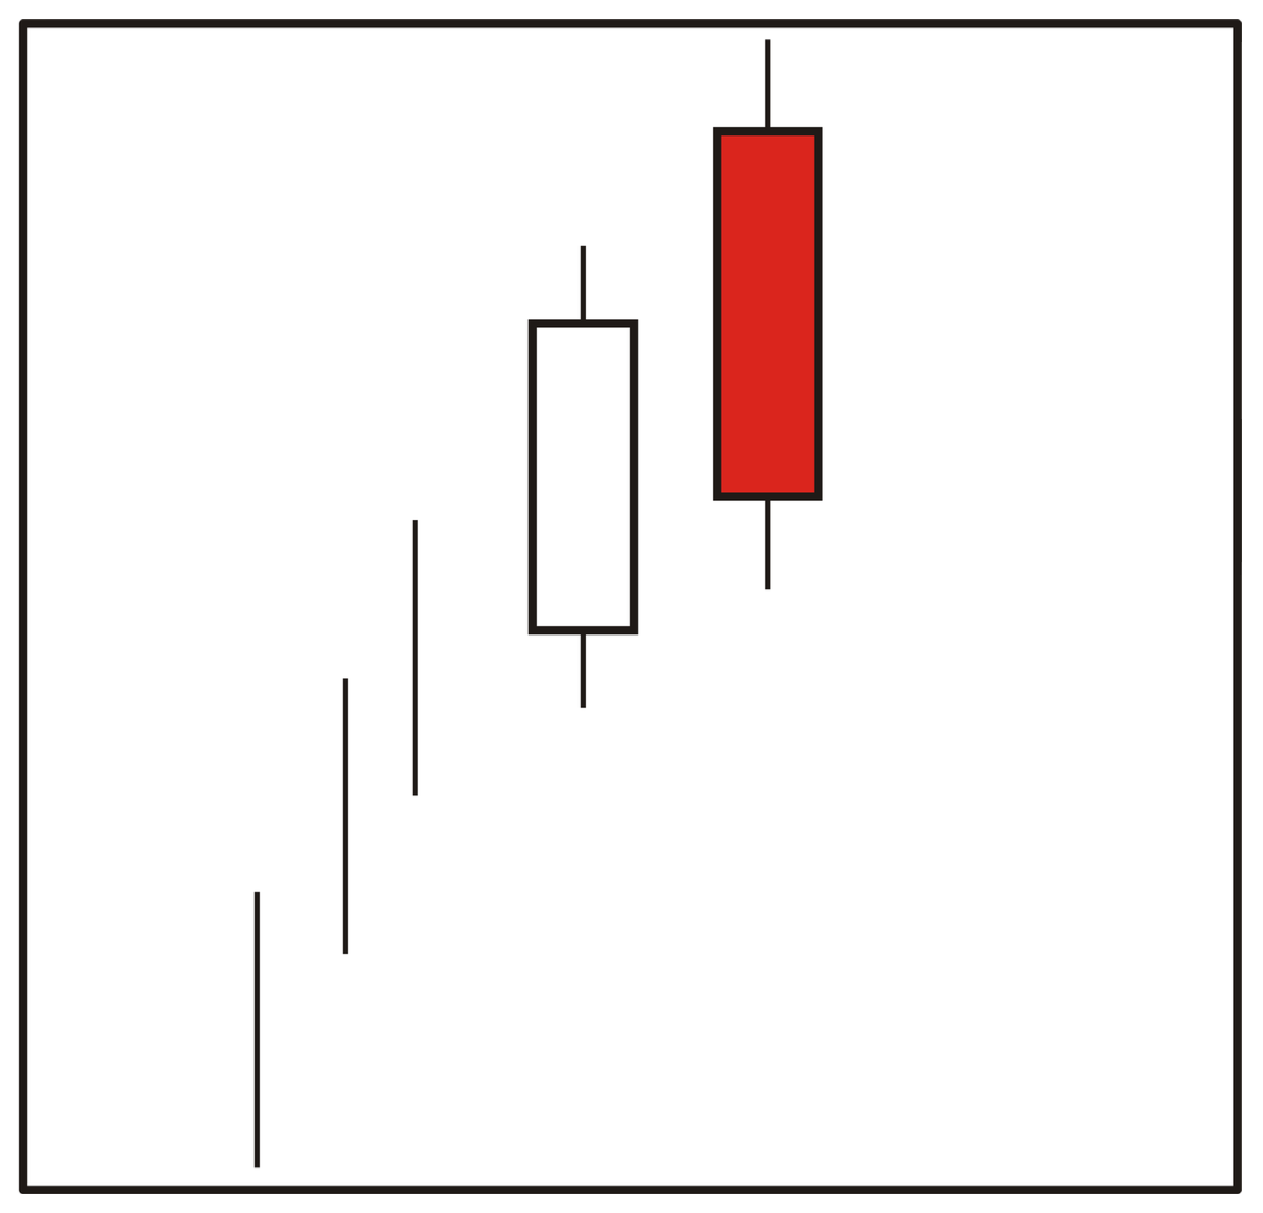
\includegraphics[width=0.5\textwidth]{figuras/f11}
\caption{Padrão DarkCloud}

\end{figure}

Diante deste cenário, criou-se a seguinte hipótese para nortear a atividade: \textit{“A implementação da prova de conceito orientada a Sistemas Multiagentes não será possível ou mesmo demandará muito esforço por parte do desenvolvedor, impossibilitando o seu uso no contexto em estudo neste TCC”}.Iniciaram-se, assim,as outras etapas ilustradas na Figura 9.

\subsection{Selecionar ativos}

Nesta etapa, foram obtidos os dados históricos dos ativos (i.e. Ações) das seguintes empresas: (i) Brookfield Incorporações,BISA3 SA; (ii) MVR Engenharia, MRVE3SA; e (iii) Rossi Residencial S.A.,RSID3SA. Para realizar a atividade com os dados disponíveis aos produtos de Software escritos na linguagem Mql4, foi feita uma coleta de dados do par de moedas Euro/Dólar americano (EUR/USD). Oscódigos Mql4, Java+JADE e Python implementados neste estudo de caso estão disponíveis nos apêndices B,C e D, respectivamente. O período adotado para coleta foi o diário entre fevereiro de 2008 e janeiro de 2014.



\subsection{Implementar Algoritmo}

Considere a candlestick de baixa na Figura 12(\ref{f12}) como candlestick 0, e a candlestick de alta como candlestick 1. De acordo com o cenário exposto no subtópico \textbf{4.1.2}, a formação é considerada Darkcloud se:

\begin{itemize}
  \item A candlestick 1 deve ser de alta;
  \item A candlestick 0 deve ser de baixa;
  \item A candlestick 0 deve ter valor de abertura superior ao valor de fechamento da candlestick 1;
  \item A candlestick 0 deve ter seu valor de fechamento entre o valor mediano do corpo da candlestick 1. Deve também ter seu valor de fechamento superior ao valor de abertura da candlestick 1;
  \item A candlestick 0 deve ter um corpo considerável.
\end{itemize}

\begin{figure}[h]
\centering
\label{f12}
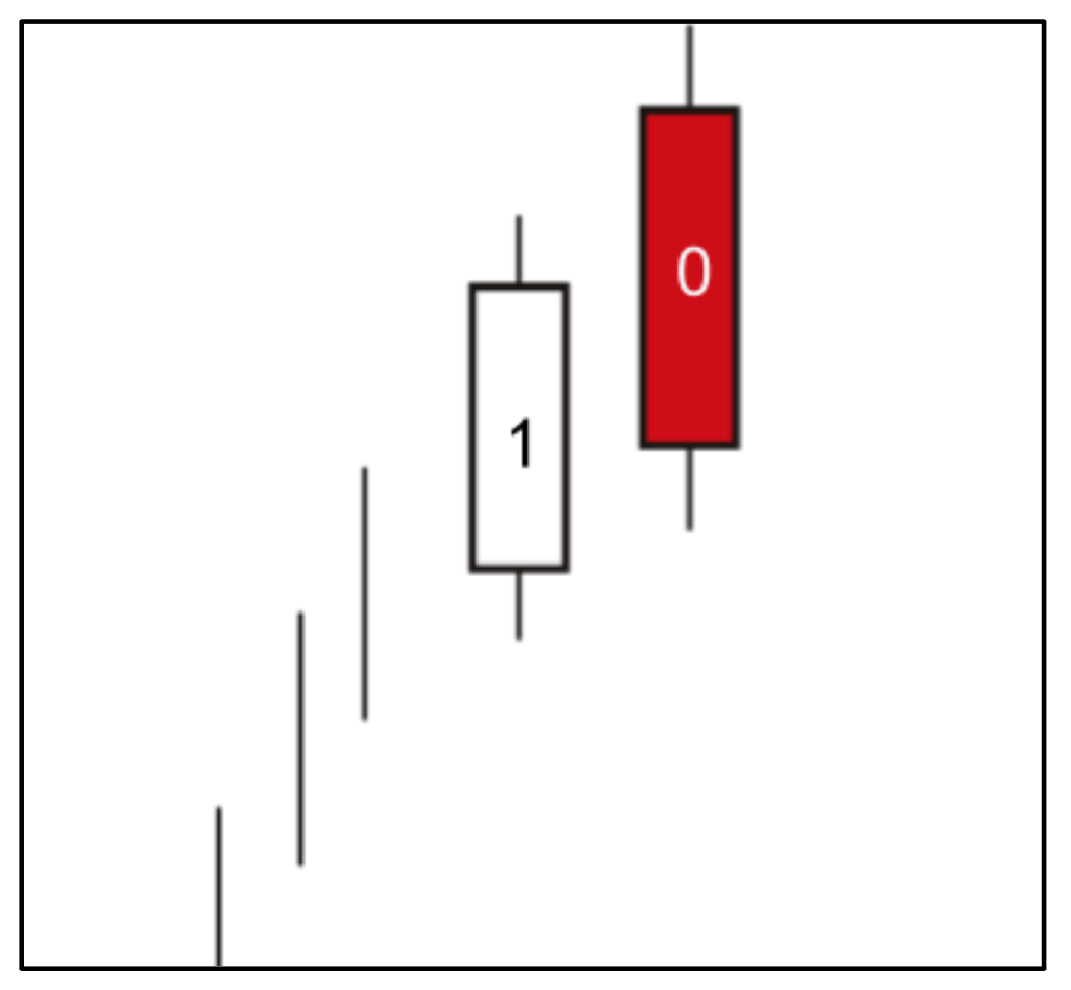
\includegraphics[width=0.5\textwidth]{figuras/f12}
\caption{DarkCloud}
\end{figure}

A Tabela 1 (\ref{t01}) apresenta o tempo gasto para implementar cada algoritmo nas linguagens eleitas para este TCC.

\begin{table}[h]
	\centering
	\label{t01}
	
	\begin{tabular}{ccc}
		\toprule
		\textbf{Linguagem} & \textbf{Tempo médio}\\
		\midrule
		Python & 2 Horas  \\
		Java + JADE & 2 Horas  \\
		MQL4 & 2 Horas  \\
		\bottomrule
	\end{tabular}

	\caption{Tempo médio de implementação do algoritmo}
\end{table}

O algoritmo foi implementado em Java com JADE em um único comportamento, onde o algoritmo concentrado em uma classe é chamado pelo agente. Na linguagem Mql4, o algoritmo implementado retorna uma sinalização visual no gráfico de candlestick, fornecido pela plataforma, alertando a identificação do padrão. Na linguagem Python, o algoritmo implementado retorna uma listagem, contendo informações como datas de ocorrência do padrão, no terminal da IDE utilizada para implementação. Vale ressaltar, que a implementação foi o suficiente para estimar a viabilidade em se implementar a ferramenta proposta no Paradigma de Sistemas Multiagentes.


\subsection{Analisar resultado}

Notou-se que o esforço necessário para implementar o algoritmo nas três linguagens foi aproximadamente o mesmo. Na linguagem Java+JADE e Python, por serem multiplataforma, existe a possibilidade em desenvolver a ferramenta de forma que a mesma tenha o mesmo comportamento nas plataformas mais populares existentes hoje.

Na proposta aqui apresentada, um critério de qualidade que merece atenção é a extensibilidade, visando futuras manutenções evolutivas bem como possibilitando trabalhar em mais de um contexto financeiro, como por exemplo, abordar o Mercado de Ações e o Mercado de Renda Fixa simultaneamente. Nesse caso, seria possível trabalhar em um contexto de alto risco de investimento juntamente com um de baixo risco de investimento, obtendo uma melhor gestão de recursos investidos pelo usuário.

Em relação a extensibilidade no contexto financeiro,o Paradigma de Sistemas Multiagentes adequa-se ao estudo,visto que já existe um suporte tecnológico apropriado, um framework que atende às necessidades deste TCC, no caso um suporte para troca de mensagens entre entidades de Software – no contexto abordado neste TCC, entre investidores – baseado em comunicação usando protocolos, padrões bem estabelecidos na comunidade de Software e possiblidades de extensibilidade orientadas, por exemplo, a ontologias específicas.

Um outro ponto considerado foi dado que o esforço em se implementar a prova de conceito utilizando a combinação tecnológica linguagem Java e plataforma JADE foi aproximadamente o mesmo em relação às implementações em Python ou Mql4. Portanto, pode-se concluir que a hipótese inicial não se verificou. Assim, a aplicação do Paradigma de Sistemas Multiagentes no contexto financeiro abordado é possível, compreendendo um esforço por parte do desenvolvedor muito próximo dos exigidos nas demais linguagens analisadas.

Finalmente, diante das propriedades do Paradigma de Sistemas Multiagentes, expostas no \textbf{capítulo 2, nos tópicos 2.2.1, 2.2.1.2 e 2.2.1.3} e a descrição do contexto financeiro exposta no mesmo capítulo, tópico 2.1.2, nota-se que existem características comuns entre eles. Nesse cenário, merecem menção as seguintes características:

\begin{enumerate}
\item Autonomia - não há intervenções no processo de decisão de um agente, ele toma decisões sem intervenção de outros agentes ou humanos. Da mesma maneira, um investidor humano também possui autonomia para decidir quando realizar investimentos;
\item Sociabilidade - um agente interage com outros agentes, Software ou humano, através de  algum tipo de linguagem de comunicação. Da mesma maneira, um investidor humano interage com outros atores presentes em uma bolsa de valores, seja para montar grupos, e de maneira conjunta resolver problemas que estão além das suas habilidades individuais, ou apenas para usar serviços disponibilizados por outros atores;
\item Reatividade - um agente fica situado em um ambiente e é capaz de perceber esse ambiente através de seus sensores, é capaz de responder em tempo hábil às mudanças que ocorrem nele. Da mesma maneira, um investidor percebe o ambiente de bolsa de valores no qual está inserido, através de acompanhamentos frequentes de informações que alimentam suas estratégias, e responde às mudanças ocorridas na bolsa de valores de acordo com as informações de saída de suas estratégias;
\item Assincronismo -  um agente, ao receber uma requisição, tem o poder de decidir se irá ou não atender à mesma. Adicionalmente, este agente este pode enviar uma requisição a outro agente e continuar suas atividades. Caso não seja atendido, ele tem o poder de enviar a mesma requisição a outros agentes, por exemplo, contornando o problema. Da mesma maneira, um investidor humano pode procurar um ou vários atores presentes na bolsa e escolher aquele que melhor o atende.

\end{enumerate}

Tal fato motiva a exploração do paradigma orientado a agentes no contexto financeiro abordado, tendo como objetivo contribuir com o contexto financeiro através da construção de uma ferramenta de estratégia financeira apoiada por Sistemas Multiagentes Comportamentais, onde não será exigido do usuário conhecimentos relacionados ao Mercado Financeiro. Assim, a ferramenta abstrairá a complexidade de cálculos financeiros comumente utilizados na análise técnica e delegará ao usuário somente a decisão em comprar ou vender.

\section{FERRAMENTA PROPOSTA}

A ferramenta será um Software de apoio à gestão de uma carteira de investimento, que inicialmente será composta por ações de empresas com presença na Bolsa de Valores Brasileira. Em evoluções futuras, a carteira de investimentos poderá ser composta também por: (i) Opções das mesmas empresas; (ii) Ativos na Bolsa de Mercadorias e Futuros Brasileiros; (iii) Letras de Dívida Pública e demais títulos de renda fixa. 

 A ferramenta proposta atuará considerando três tipos de perfis de investidor, de forma a contribuir na realização do maior lucro possível dentro do perfil do usuário, ou seja, sob a perspectiva de investimento cabível para esse usuário. Informações sobre os perfis são simplificadamente providas na Tabela 2.

\begin{center}
\begin{longtable}{| p{8cm} | p{8cm} |}
\caption{Perfis de investidores} \\
\hline
\textbf{Perfil } & \textbf{Descrição} \\ \hline
\endfirsthead
\multicolumn{2}{c}%
{\tablename\ \thetable\ -- \textit{Continuação da página anterior}} \\
\hline
\textbf{NomeColuna1} & \textbf{NomeColuna1} \\ \hline
\endhead
\hline \multicolumn{2}{c}{\textit{Continuaçao na próxima página}} \\
\endfoot
\hline
\endlastfoot
	Corajoso & São pessoas que, dentre os três perfis, assumem o maior risco e estão dispostas a acompanhar com maior frequência a movimentação do Mercado Financeiro.\\ \hline
	Moderado & São pessoas que estão entre os perfis Corajoso e Conservador. Esse perfil adequa-se às pessoas que desejam operar esporadicamente no Mercado Financeiro, mas com um certo nível de risco.\\\hline
	Conservador & São pessoas que desejam gerir seu próprio plano de aposentadoria complementar, utilizando o Mercado Financeiro Brasileiro.Pessoas com este perfil desejam apenas arrecadar um capital suficiente para garantir seu padrão de vida, ou seja é uma pessoa que deseja um lucro razoável com um grau de risco menor do que os outros perfis.
\label{t01}
\end{longtable}
\end{center}

Para cada perfil de investidor serão utilizados agentes com estratégias que mais se adequam ao perfil. Para o perfil Conservador serão priorizadas empresas que oferecem dividendos e aquelas que oferecem menores volatilidades bem como boa liquidez de seus papéis. Para o perfil Moderado serão priorizadas estratégias de compra e venda de papéis em uma periodicidade maior do que a semanal. E para o perfil Corajoso, serão utilizadas estratégias de curto prazo, ou seja, entre um dia e quatro semanas. O tópico a seguir expõe algumas estratégias utilizadas por investidores e algumas que podem ser adotadas por este estudo.

\subsection{Principais Agentes}

Como proposta inicial deste TCC, serão implementados três grupos de agentes. Um grupo de gestores, um grupo de especialistas de operação e um grupo de caçadores de papéis (i.e. ações de empresas),Figura 13(\ref{f13}). Um agente do grupo de gestores é responsável por controlar investimentos para que eles estejam em um grau de risco aceitável ao usuário investidor, seja ele Corajoso, Moderado ou Conservador. Esse agente terá uma equipe formada por agentes dos grupos de especialistas operação e de caçadores de papéis.

Os Agentes Caçadores de papéis ficarão responsáveis por procurar no Mercado Financeiro Brasileiro papéis que sejam interessantes para o perfil do usuário investidor, fazendo uma seleção de papéis e passando essas informações para o agente gestor de um grupo de especialistas. Esses últimos farão uso das estratégias financeiras expostas no \textit{tópico 4.2.5.1}. Os agentes serão construídos de forma que seja possível continuar o estudo futuramente, mantendo ativo o critério de qualidade: manutenibilidade evolutiva do Software desenvolvido.

Os Agentes Especialistas ficarão responsáveis por monitorar um grupo de ações passados pelo seu gestor, eles monitorarão a variação de preços das ações sob sua custódia.

\begin{figure}[h]
\centering
\label{f13}
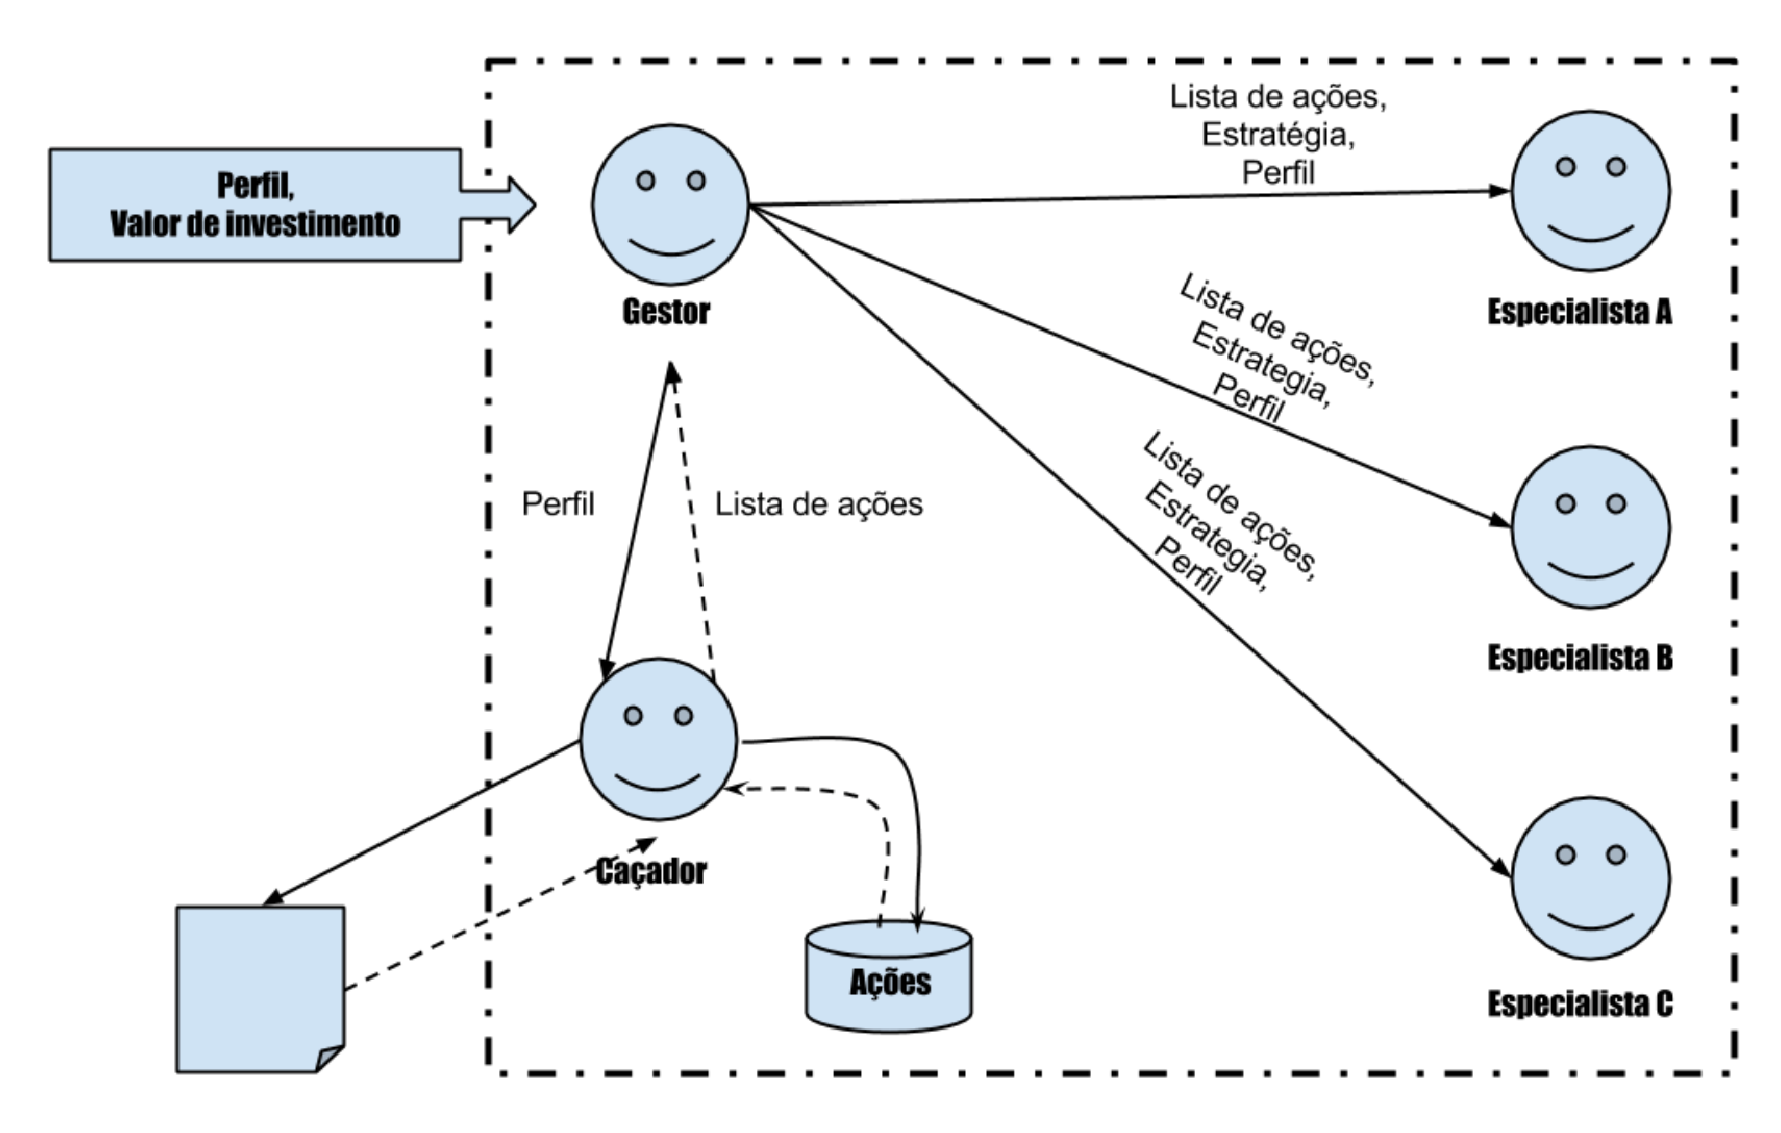
\includegraphics[width=0.8\textwidth]{figuras/f13}
\caption{Estrutura de agentes planejado }

\end{figure}

\subsubsection{Agente Gestor}
O Agente Gestor irá administrar uma equipe composta por um ou mais especialistas. Ele autorizará uma compra ou venda de ações analisadas pelos especialistas. Ele fará controle constante do risco envolvido na carteira de ações administrada. O Agente Gestor de riscos tem as principais responsabilidades:
\begin{enumerate}
\item Criar e excluir um ou mais Agentes Especialistas;
\item Autorizar compras ou vendas de ações;
\item Monitorar os riscos envolvidos na carteira de ações, bem como alinhar estes ao perfil do usuário investidor;
\item ntervir, se necessário, em uma operação que represente altos riscos.
\end{enumerate}

As responsabilidades dos Agentes gestores relacionadas à gestão da carteira de investimento estão descritas no \textit{tópico 4.2.3}.

\subsubsection{Agente Especialista}

O Agente Especialista é o agente que fará constantemente leituras dos valores das ações que estão sob sua responsabilidade. Ele receberá uma lista de ações do Agente Gestor e aplicará a melhor estratégia possível para cada ação. Ele fará o cálculo do risco envolvido em suas estratégias, orientados por em uma base histórica de operações e/ou simulações feitas em valores históricos desta ação. O Agente Especialista tem as seguintes responsabilidades:

\begin{enumerate}
\item Aplicar estratégias que ofereçam o maior lucro possível para cada tipo de usuário investidor;
\item Mensurar o risco envolvido em cada estratégia e reportar ao Agente Gestor;
\item Fazer simulações e persistir informações de operações;
\end{enumerate}

\subsubsection{Agente Caçador}

O Agente Caçador de papéis fará buscas constantes no portfólio de ações da bolsa  de valores, afim de selecionar as que mais oferecem retornos positivos. Após encontrar estes papéis, ele informará aos Agentes Gestores. O Agente Caçador de papéis tem as seguintes responsabilidades: 
\begin{enumerate}
\item Buscar e selecionar as melhores ações a se investir;
\item Criar uma listagem destas ações e reportar aos Agentes Gestores que solicitarem.
\end{enumerate}

\subsubsection{Gestão de Carteira dos Agentes Gestores}

De acordo com o perfil do usuário, os Agentes Gestores farão a gestão da carteira de investimento usando duas estratégias, gestão passiva e ativa. Para o investidor Conservador, ele fará uma gestão mais passiva, onde não há intenção de sobrepor o mercado. A carteira será mais diversificada e as ações permanecerão compradas por um tempo maior, consequentemente o risco envolvido será menor, em relação aos outros perfis.

Para o investidor Moderado, ele fará uma gestão um pouco mais ativa, onde há uso de estratégias financeiras para tentar se antecipar ao mercado, no entanto com um controle de risco mais rigoroso do que perfil Corajoso. Para o perfil Corajoso, os Agentes Gestores adotarão uma gestão mais ativa. A carteira de ações de um usuário corajoso possui uma diversificação menor e o controle de risco é menos rigoroso em relação aos outros perfis.

Para gerir uma carteira, o Agente Gestor calculará constantemente o desvio padrão e a variância da carteira, bem como das Ações individualmente. Ao montar uma carteira de ações, os Agentes Gestores usarão como parâmetro a correlação entre as ações da carteira, além do perfil do usuário. Os subtópicos seguintes expõem o procedimento de montagem e monitoração de uma carteira de ações gerida por um Agente Gestor.

\subsubsubsection{Montagem da carteira de ações}

Após instanciado os agentes para o usuário, o Agente Gestor verifica qual foi o perfil escolhido pelo usuário em seu cadastro e inicia o processo de montagem de carteira de ações. Ele contata um Agente Caçador e solicita um número determinado de ações, de acordo com o perfil do usuário. Segundo Pinheiro (\citeyear{pinheiro2008},p.93),uma carteira com ações de 30 empresas diferentes pode ser considerada como uma carteira conservadora. Com base neste número, foi derivada a quantidade de ações por carteira de cada tipo de perfil. Assim, para um usuário Conservador sua carteira terá ações de 30empresas. Para um Moderado 13 empresas. E para um usuário Corajoso 8 empresas. Vale ressaltar que esses números são iniciais foram baseados na recomendação do autor Pinheiro (\citeyear{pinheiro2008},p.93) combinados com os números da sequência de Fibonacci, sequência bastante aceita no meio financeiro, e serão ajustados empiricamente durante TCC2.


\begin{figure}[h]
\centering
\label{f14}
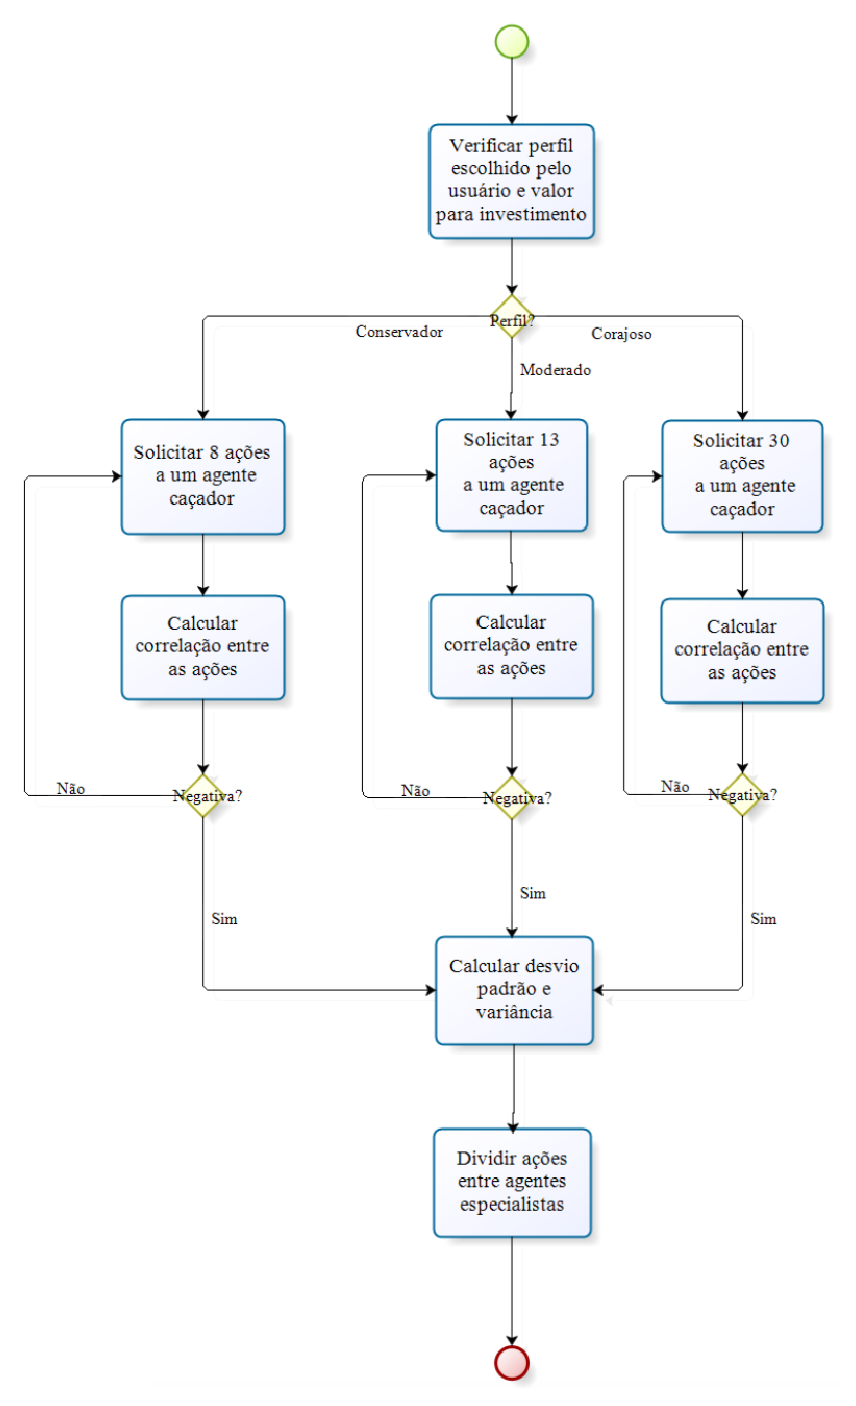
\includegraphics[width=0.8\textwidth]{figuras/f14}
\caption{Processo de montagem de uma carteira}

\end{figure}


Ao receber o grupo de ações solicitadas ao Agente Caçador, o Agente Gestor calcula a correlação dos retornos (i.e. percentual de diferença entre o período atual com seu anterior) e as aprova de acordo com o perfil do usuário. Os critérios de aceite de uma ação é mostrado na Tabela 3.

\textbf{Tabela 3: Critério de aceite de ações}

\begin{center}
\begin{longtable}{| p{2cm} | p{2cm} |p{2cm} |p{2cm} |}
\caption{Critério de aceite de ações} \\
\hline
\textbf{Perfil} & \textbf{Quandidade de empresas} & \textbf{Critério de aceite} & \textbf{Tolerância} \\ \hline
\endfirsthead
\multicolumn{2}{c}%
{\tablename\ \thetable\ -- \textit{Continuação da página anterior}} \\
\hline
\textbf{NomeColuna1} & \textbf{NomeColuna2} & \textbf{NomeColuna3} & \textbf{NomeColuna4}\\ \hline
\endhead
\hline \multicolumn{2}{c}{\textit{Continuaçao na próxima página}} \\
\endfoot
\hline
\endlastfoot
	Corajoso & 8 & Correlação negativa & Dois pares de ações com correlação positiva.\\ \hline
	Moderado & 13 & Correlação negativa & Um par de ações com correlação positiva.\\ \hline
	Conservador & 30 & Correlação negativa & Nenhuma.\\ \hline
\label{t03}
\end{longtable}
\end{center}



Após feito cálculo da correlação, o Agente Gestor calcula o desvio padrão e a variância dos retornos da ação e distribui entre os Agentes Especialistas que compõem sua equipe.

\subsubsubsection{Monitoramento da carteira de Ações}

Ao montar a carteira de ações e dividir as ações entre os Agentes Especialistas, os Agentes Gestores iniciarão o processo de monitoramento desta carteira. Eles solicitarão o percentual de retorno aos Agentes Especialistas, de acordo com a periodicidade trabalhada. Ao obter os valores, os Agentes Gestores realizarão o cálculo da correlação e desvio padrão para encontrar ações que representem risco em desacordo com o perfil do usuário. Se a ação representar um risco elevado, esta será removida da carteira e possivelmente substituída.

\begin{figure}[h]
\centering
\label{f15}
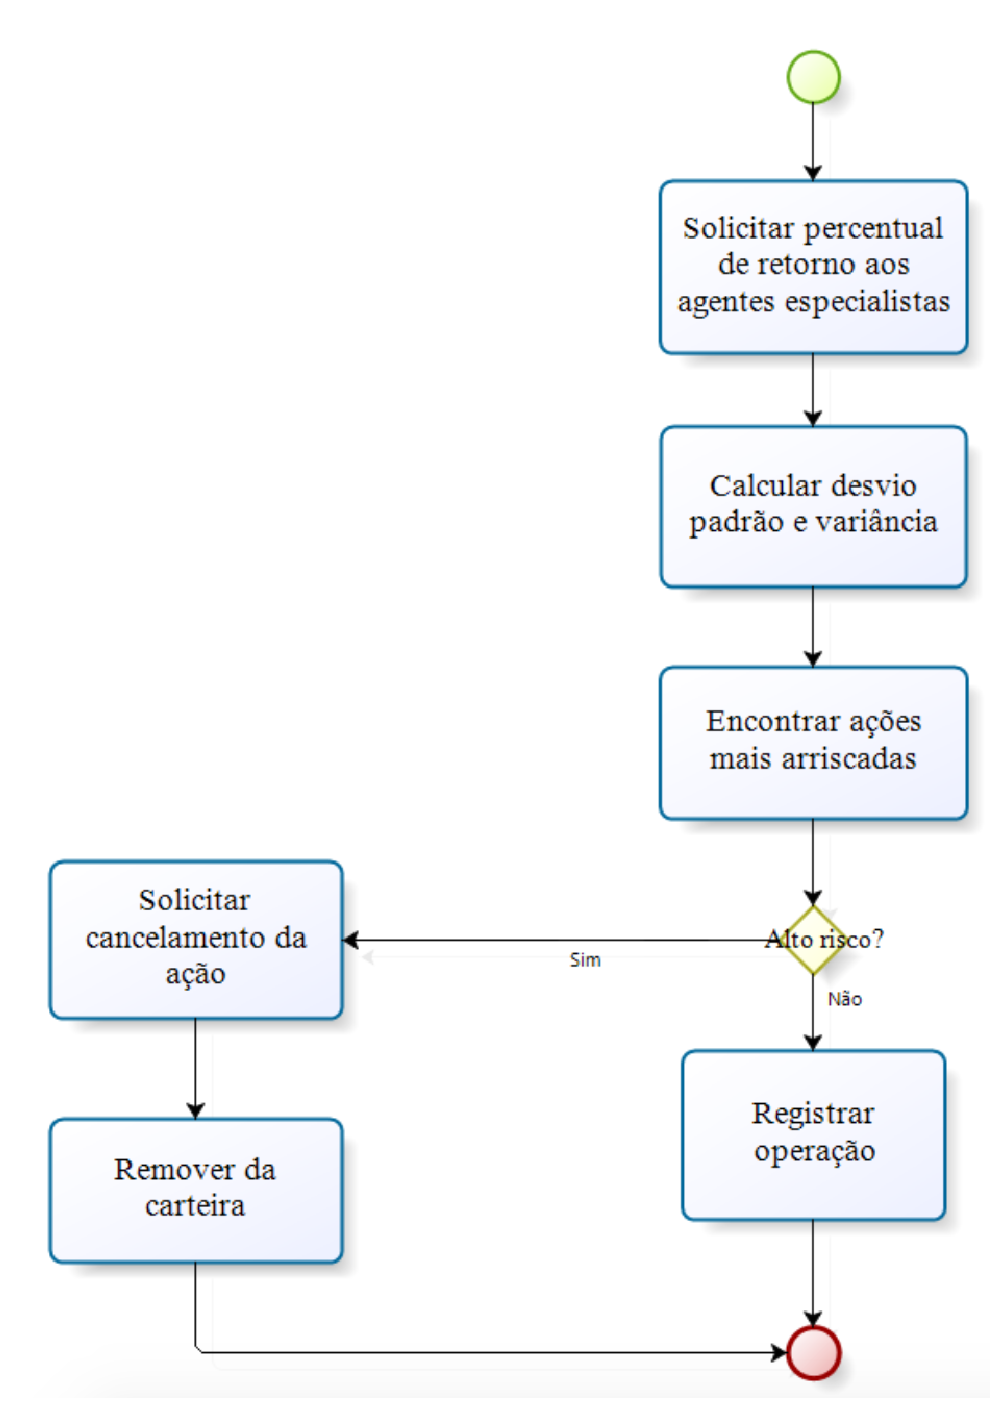
\includegraphics[width=0.8\textwidth]{figuras/f15}
\caption{Processo de monitoramento da carteira}
\end{figure}

\subsubsection{Estratégias de busca de ações dos Agentes Caçadores}

Os Agentes Caçadores farão buscas de ações constantemente na bolsa de valores. Eles farão leituras dos dados históricos de cada ação e persistirão uma base de dados com informações como o Retorno diário,o Desvio padrão, e a Variância. Todos na periodicidade diária, semanal e mensal. Adicionalmente, será persistido  o link para acesso à cotação pelos Agentes Especialistas.

\subsubsection{Estratégia dos Agentes Especialistas}

Com intuito de se obter um Software que ofereça uma melhor manutenção, serão adotados padrões de projeto. Visando exemplificar o uso de padrões de projeto no cenário acordado, será adotado, por exemplo, o padrão de projeto comportamental Strategy. Esse padrão permite a variação de algoritmos, independentemente do agente, facilitando ainda ser sensível ao contexto. O padrão Strategy é composto por três participantes: (i) Context, é quem chama uma estratégia através uma classe interface. Neste estudo,Context será representado pelos agentes, os quais avaliarão, em tempo de execução, o cenário financeiro vivenciado pelo investidor; (ii) Strategy, é a interface comum a todos os algoritmos relacionados à ela; e (iii) ConcreteStrategy, é a classe concreta que implementa os diferentes algoritmos. Neste estudo, serão as estratégias financeiras com as quais os agentes financeiros atuarão no ambiente. A Figura 16 (\ref{f16}) mostra como esse padrão é aplicado/instanciado considerando a ferramenta proposta.

\begin{figure}[h]
\centering
\label{f16}
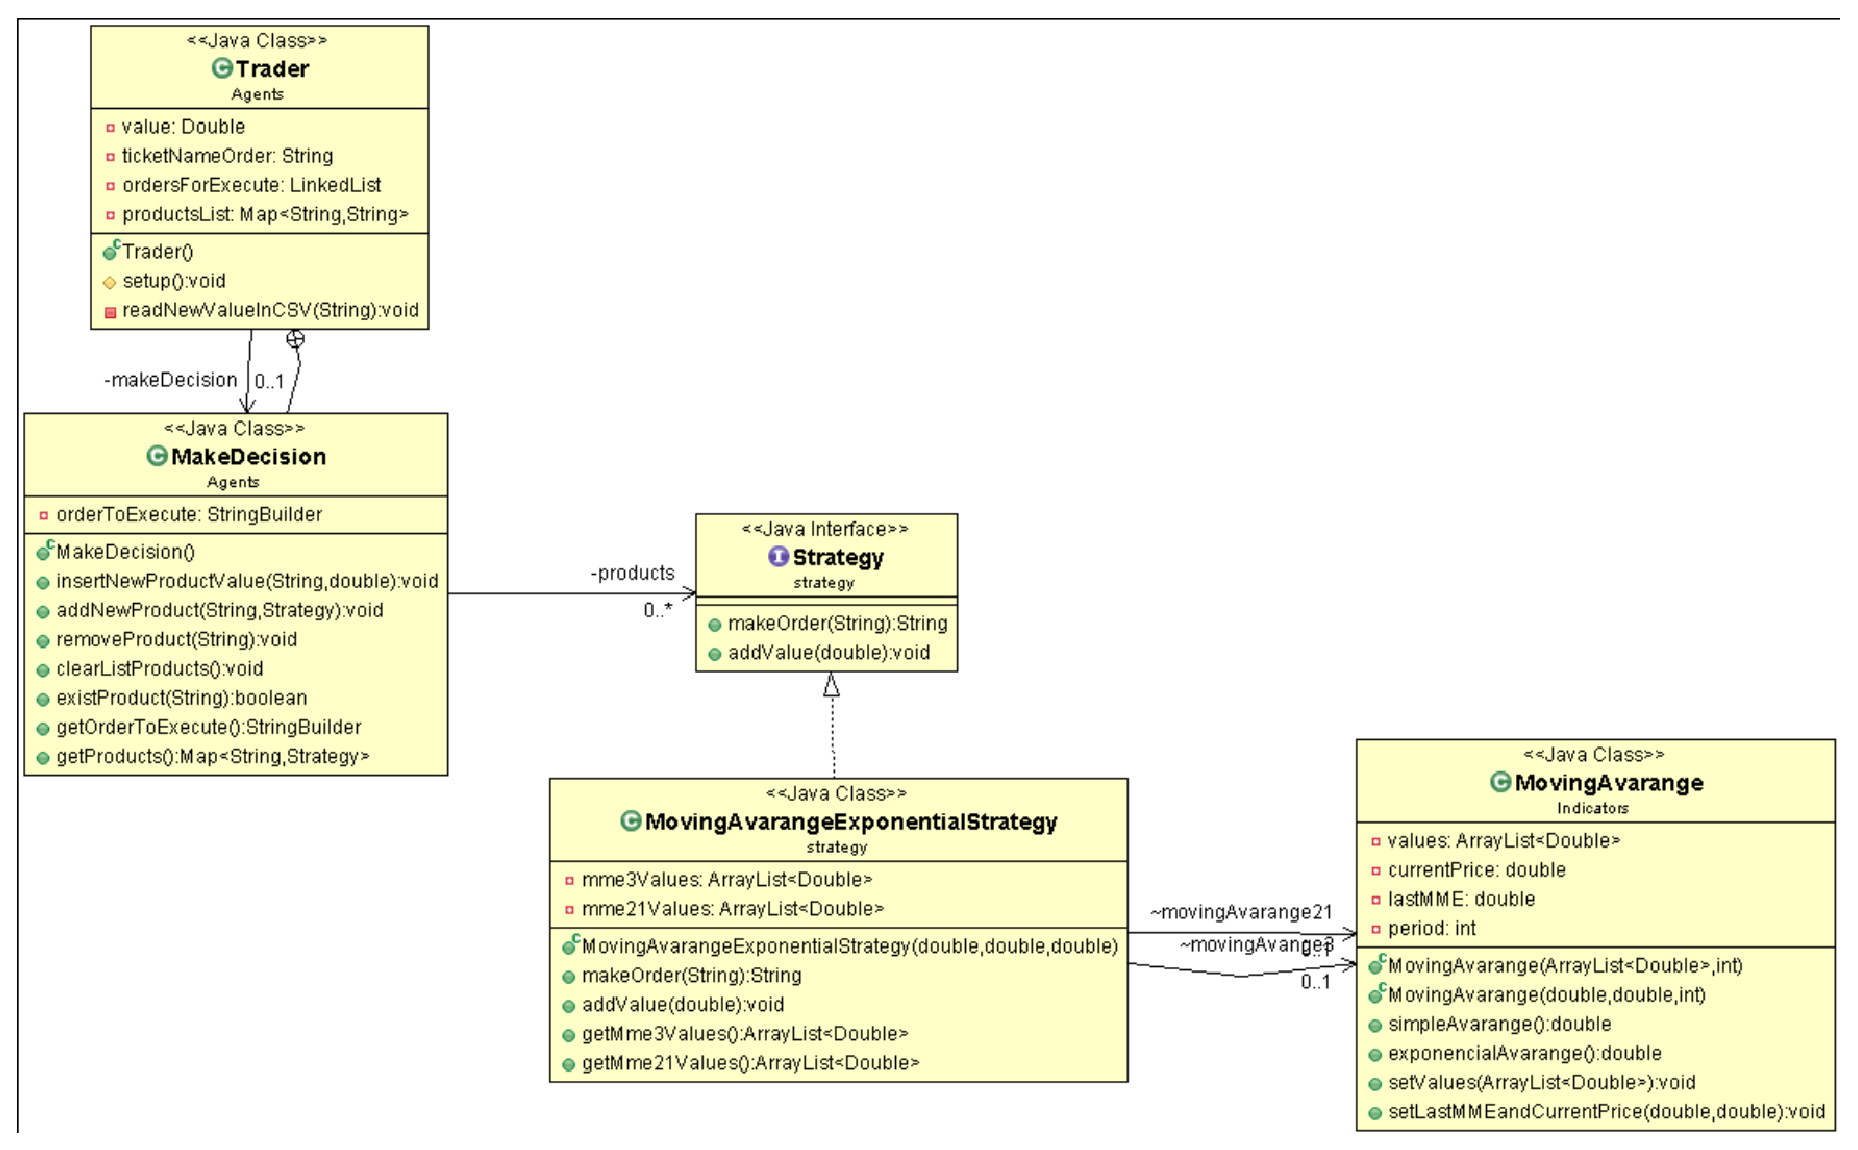
\includegraphics[width=0.8\textwidth]{figuras/f16}
\caption{Padrão Strategy aplicado}
\end{figure}


Por fim, os Agentes Especialistas farão uso de estratégias financeiras. Estratégias estas compostas por indicadores financeiros. Assim, será necessário neste estudo implementar estratégias financeiras em linguagem Java para que as mesmas possam ser utilizadas por estes Agentes.  Serão implementados, inicialmente, os seguinte indicadores: (i) Média Móvel Simples, MMS; (ii) Média Móvel Exponencial, MME; (iii) Darkcloud; (iv) Bullishengulfing  e (v) BearishEngulfing. Estes, descritos a partir do \textbf{tópico 4.2.4.1}. Serão implementadas ainda, classes que representam estratégias financeiras que farão uso de combinações destes indicadores, como apresentado na Tabela 4.


\begin{center}
\begin{longtable}{| p{2cm} | p{1cm} |p{2cm} |p{3cm} |}
\caption{Estratégias por perfil} \\
\hline
\textbf{Perfil} & \textbf{Estratégia 1} & \textbf{Estratégia 2}& \textbf{Estratégia 3}\\\hline
\endfirsthead
\multicolumn{2}{c}%
{\tablename\ \thetable\ -- \textit{Continuação da página anterior}} \\\hline
\textbf{Perfil} & \textbf{Estratégia 1} & \textbf{Estratégia 2} & \textbf{Estratégia 3} \\ \hline
\endhead
\hline \multicolumn{2}{c}{\textit{Continuaçao na próxima página}} \\
\endfoot
\hline
\endlastfoot
	Corajoso & MME (13/21) & Dark Clould + Bullish Engulfing. & Bearish Engulfing + Bullish Engulfing\\ \hline
	Moderado & MMS(13/21) & MME(13/21) & MME(13/21) \\\hline
	Conservador & MMS(13/21) & MMS(21/34)& MME(21/34)

\label{t04}
\end{longtable}
\end{center}

\subsubsubsection{Estratégias Financeiras}

Existem duas formas de se fazer investimentos no Mercado Financeiro. A primeira é investir sem nenhum critério, de forma Ad Hoc, e a outra é investir orientando-se por planos de estratégias. Um plano de estratégia deve ser montado de acordo com o nível de risco assumido pelo investidor. Um plano pode ser orientado por outros tipos de indicadores, além dos adotados nesse estudo.

Neste estudo, serão usadas estratégias financeiras baseadas em médias móveis exponenciais e simples, inicialmente. Serão duas médias de duas periodicidades, onde o cruzamento indica reversão no sentido do mercado (MATSURA, 2006, p. 72). No cruzamento da média de menor periodicidade com a maior, de baixo para cima, serão feitas ordens de compra de ações. Já no cruzamento inverso, serão feitas vendas.

\subsubsubsection{Estratégias Baseadas em Médias Móveis}

São utilizadas, como ilustrado na Figura 17 (\textbf{f17}), duas médias móveis exponenciais, uma de 21 períodos na cor azul e uma de 13 períodos na cor vermelha, a titulo de exemplo. Na estratégia de cruzamento de médias móveis, o cruzamento da vermelha com a azul, de cima para baixo, como mostrado nos círculos pretos, indica oportunidade de venda de ações. No cruzamento da vermelha com a azul, de baixo para cima, indica oportunidade de compra de ações. No \textbf{tópico 4.2.5}, estão expostos os tipos de médias móveis e suas utilizações.

\begin{figure}[h]
\centering
\label{f17}
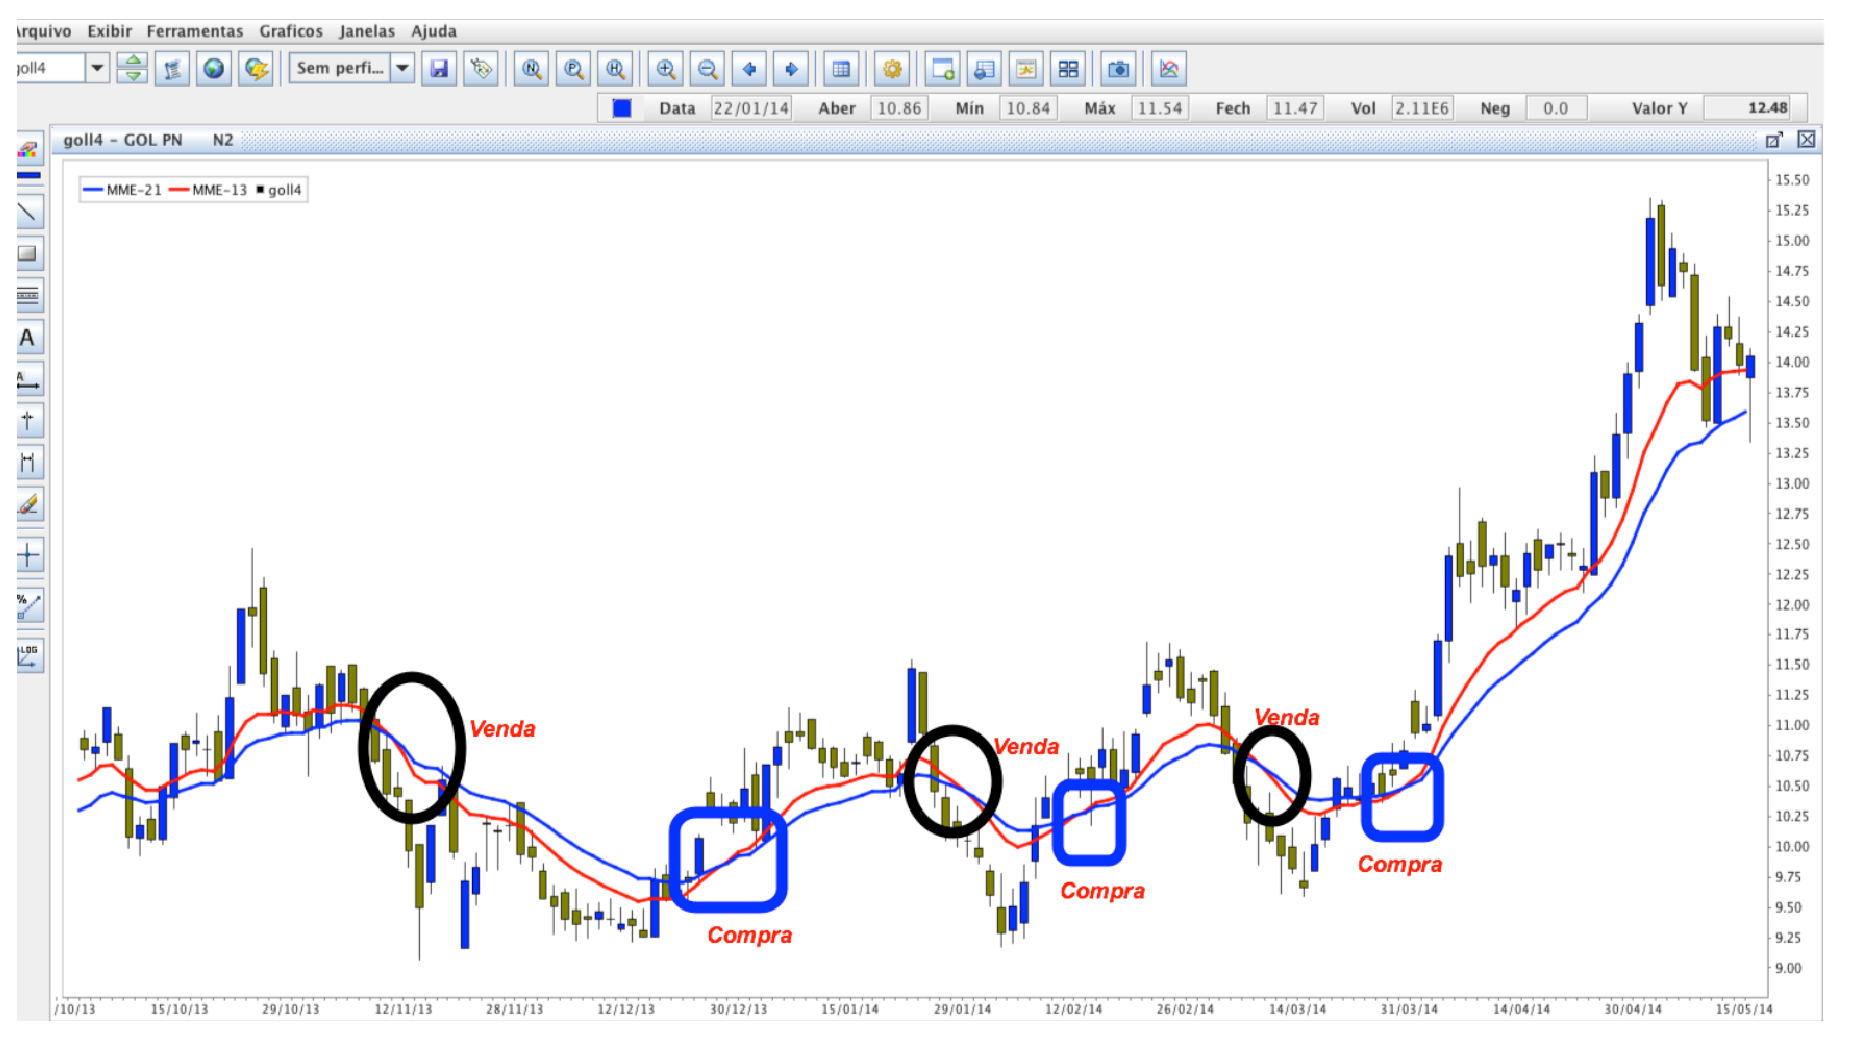
\includegraphics[width=0.8\textwidth]{figuras/f17}
\caption{Ações Gol Linhas Aérias}
\end{figure}


\subsubsubsection{Estratégias Baseadas em padrões de candlestick}

Esta estratégia foi elaborada com base no uso do gráfico de candlesticks (veja a definição de candlestick no item 4.1.1) e consiste na utilização de três padrões de formação de candlesticks. Nessa última, quando identificada a formação no gráfico da ação, é feita uma operação de compra ou de venda. A Figura a seguir apresenta estes três padrões, que serão adotados neste estudo.

\begin{figure}[h]
\centering
\label{f18}
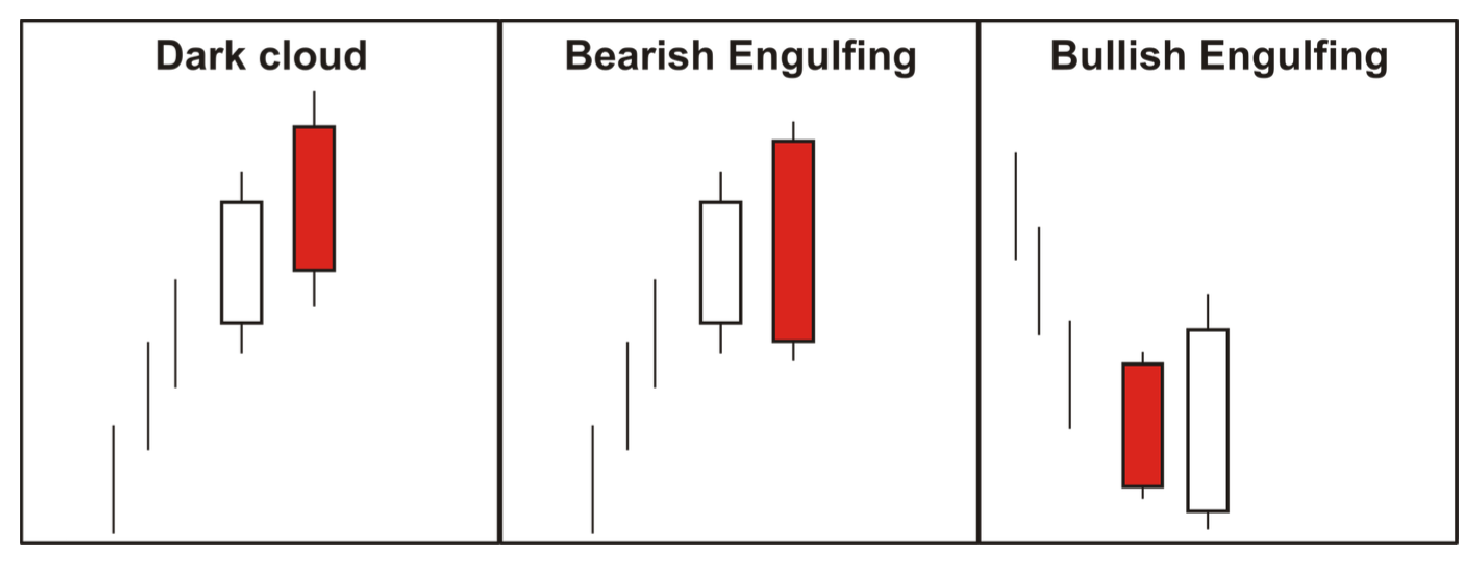
\includegraphics[width=0.8\textwidth]{figuras/f18}
\caption{Padrões de formação de candlestick}
\end{figure}


O padrão de formação Darkcloud é composto por duas candlesticks, a primeira de alta, em branco, e a segunda de baixa, em vermelho. Elas são precedidas de uma tendência de alta confirmada da ação. A segunda candlestick tem valor de abertura superior ao valor de fechamento da primeira, e tem valor de fechamento superior ao valor de abertura da primeira candlestick. Este padrão de formação indica reversão da tendência de alta para baixa \cite[p.61]{matsura2006}. Tal fato será utilizado para sinalizar oportunidades de venda de ações.

O padrão de formação BearishEngulfing, assim como o Darkcloud, sinaliza a reversão de um tendência de alta de uma ação. No entanto, este padrão difere-se por sua segunda candlestick ter valor de fechamento inferior ao valor de abertura da primeira \cite[p. 38]{bigalow2010}.

O padrão de formação BullishEngulfing é um padrão de reversão de tendência similar ao BearishEngulfing. Este padrão é precedido de uma tendência de baixa, e sinaliza oportunidade de compra de ações. É composto por duas candlesticks, a primeira de baixa fecha de acordo com a tendência (i.e. uma candlestick de baixa). A segunda tem seu valor de abertura inferior ao valor de fechamento da primeira, e seu valor de fechamento maior do que o valor de abertura da primeira \cite[p. 36]{bigalow2010}. As Figuras 19 a 21 (\ref{f19},\ref{f20},\ref{f21}) apresentam os padrões identificados em um gráfico de candlesticks.

\begin{figure}[h]
\centering
\label{f19}
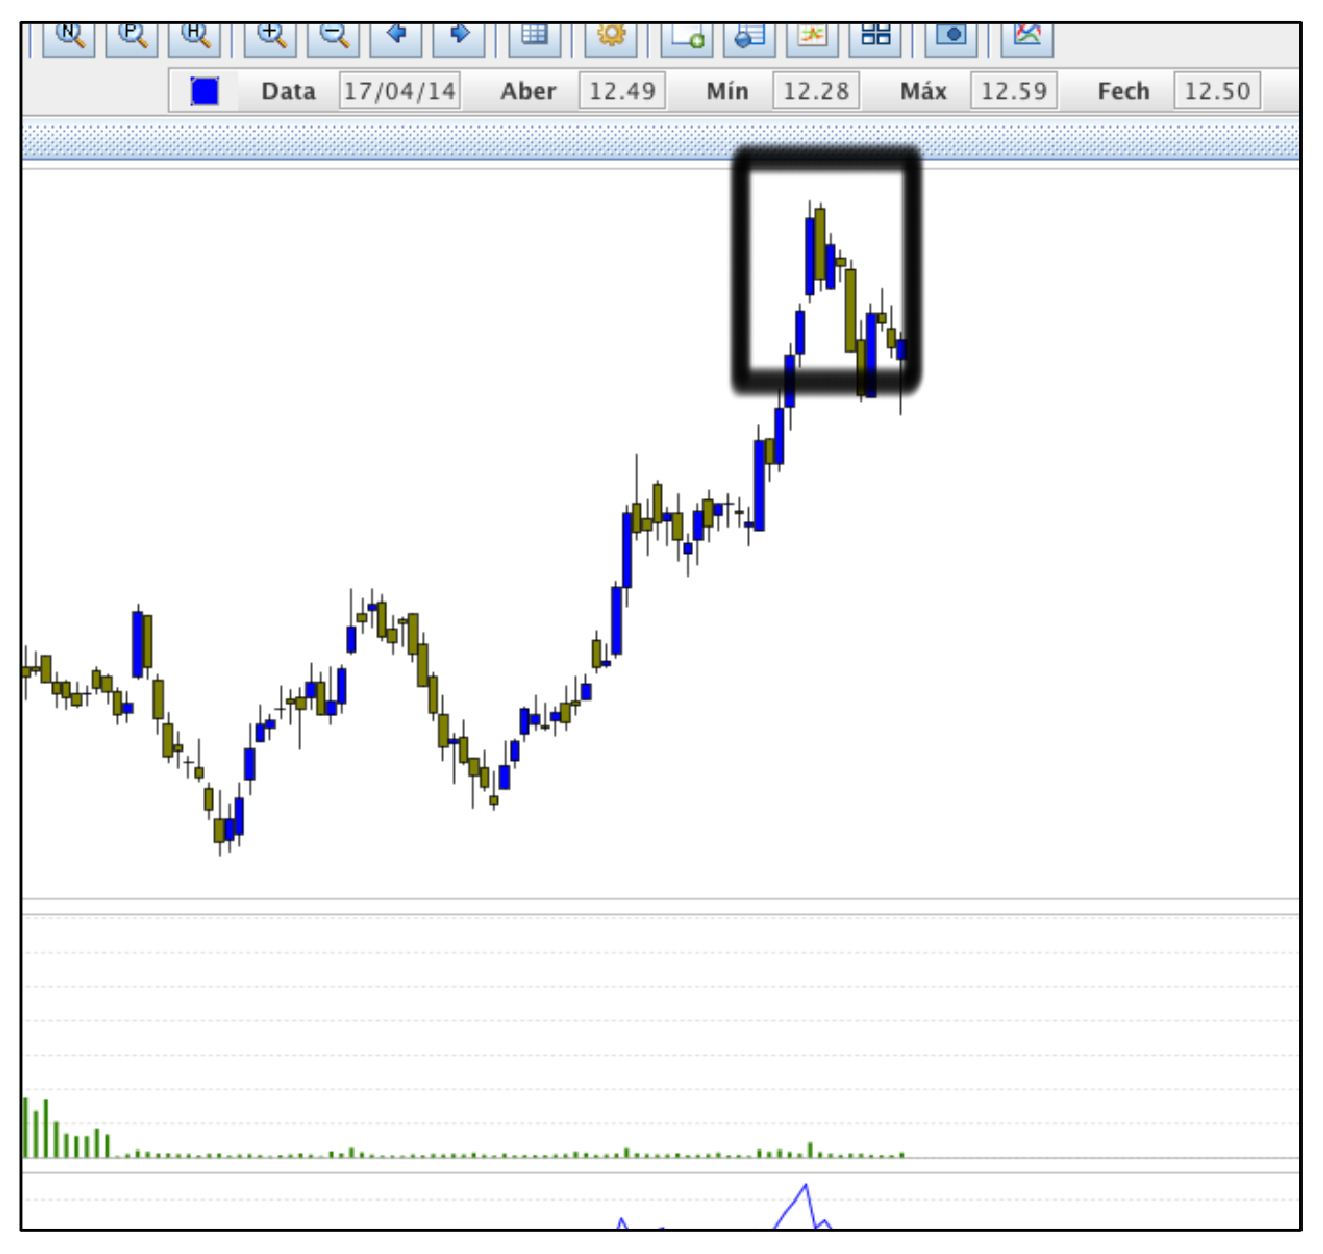
\includegraphics[width=0.8\textwidth]{figuras/f19}
\caption{Padrão DarkCloud}
\end{figure}

\begin{figure}[h]
\centering
\label{f20}
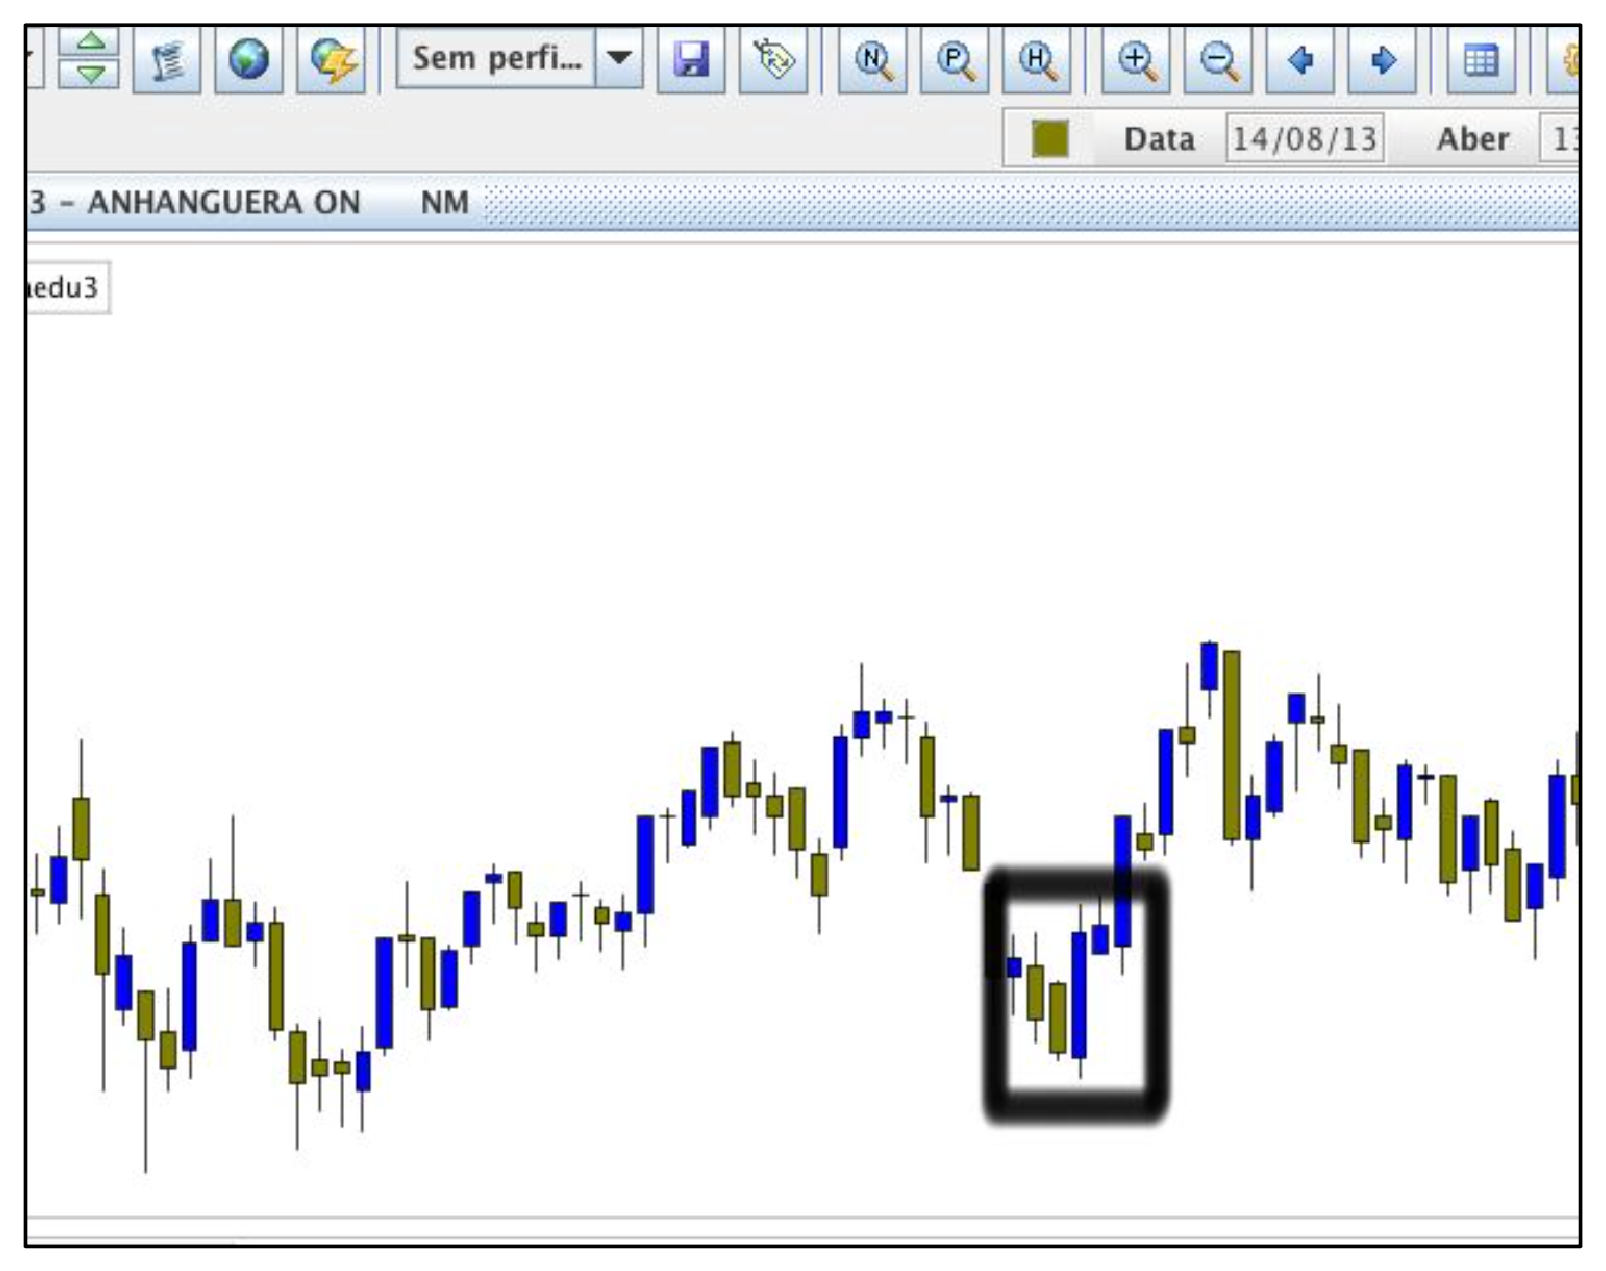
\includegraphics[width=0.8\textwidth]{figuras/f20}
\caption{Padrão Bullish Engulfing}
\end{figure}

\begin{figure}[h]
\centering
\label{f21}
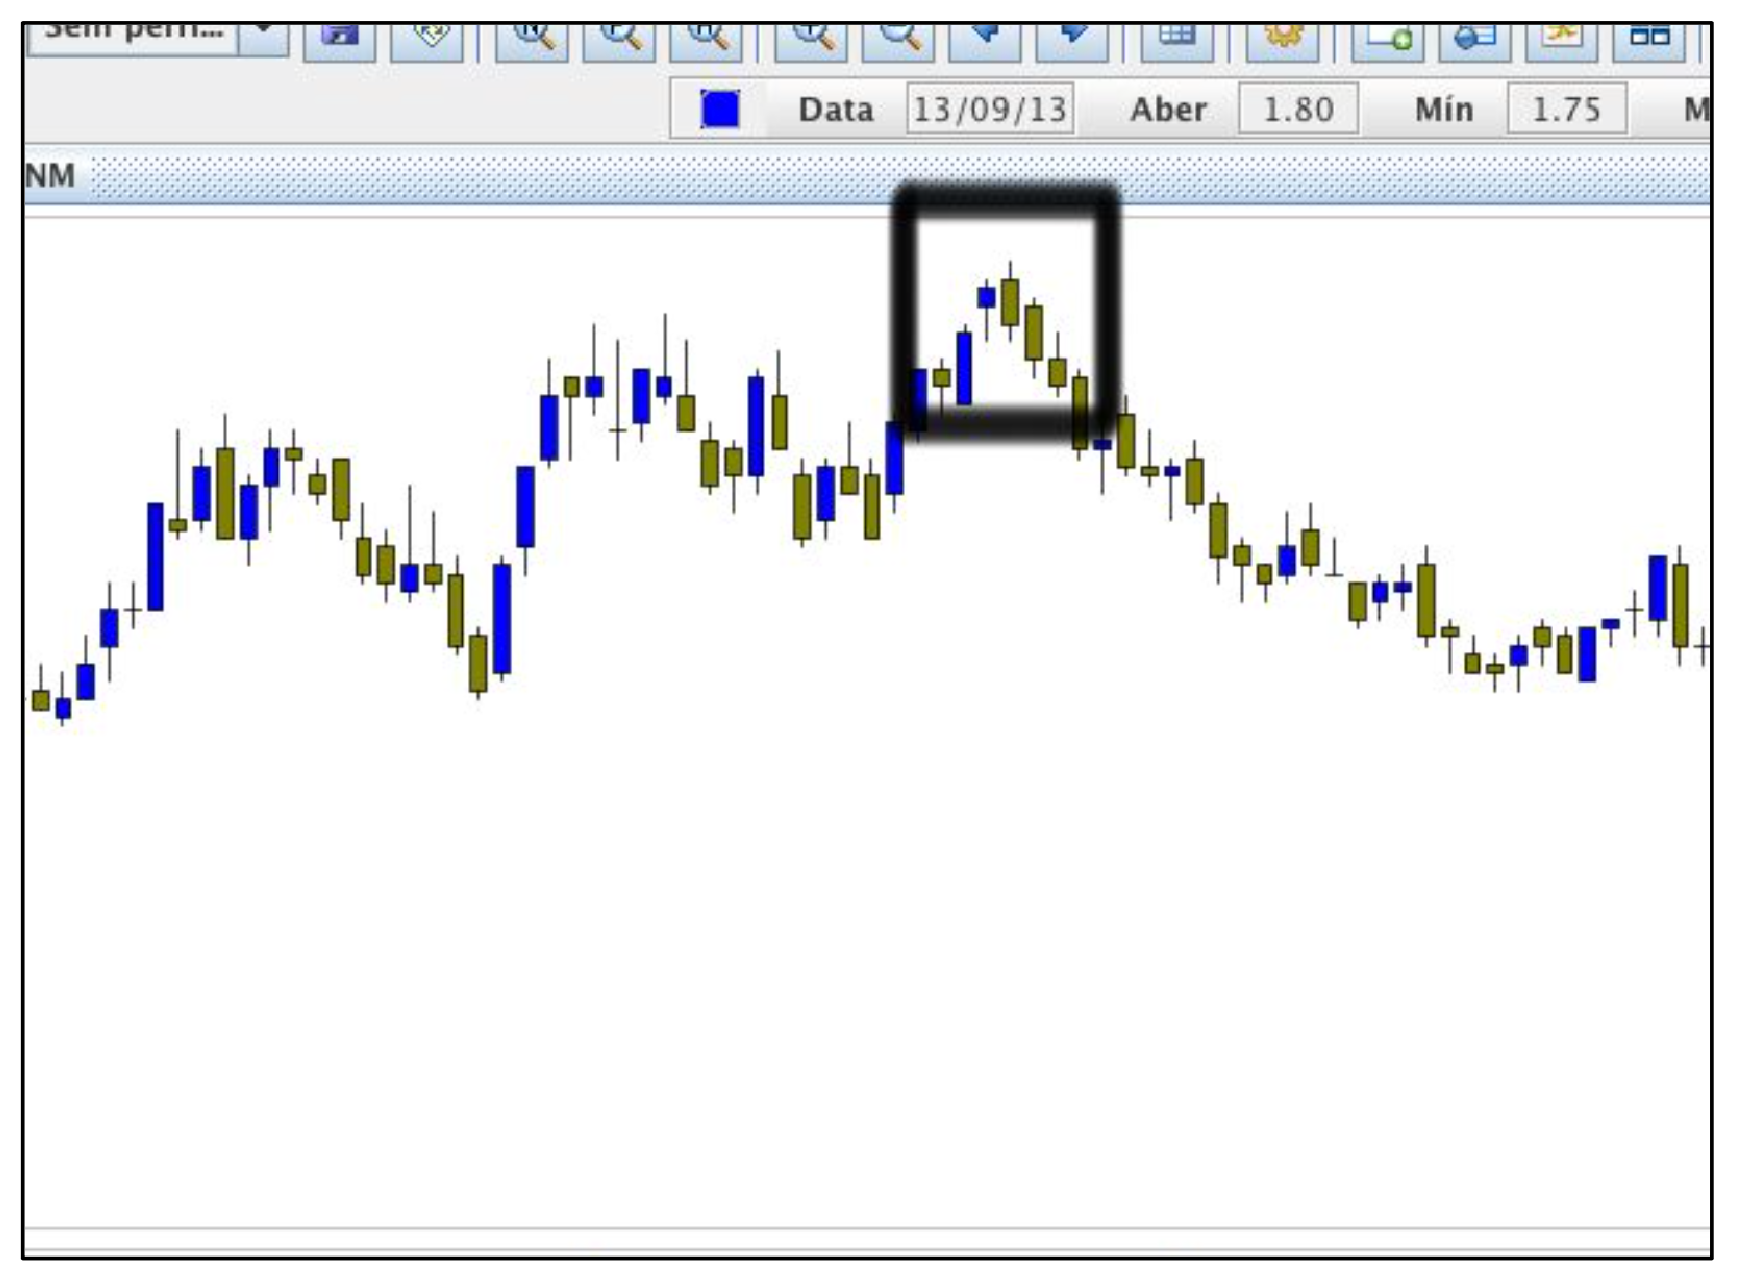
\includegraphics[width=0.8\textwidth]{figuras/f21}
\caption{Padrão Bearish Engulfing}
\end{figure}

\subsubsubsection{Médias Móveis}

Médias móveis são médias de preços que se deslocam no tempo, ou seja, para um novo valor de entrada, há a saída de um valor antigo do cálculo. Com as médias móveis é possível suavizar a movimentação do mercado e, dessa forma, identificar tendências \cite[p.68]{matsura2006}. Ao se calcular uma média móvel, é escolhido primeiro qual a quantidade de valores que será utilizado no cálculo. Se utilizamos 5 valores, tem-se, então, uma média de 5 períodos, e assim por diante. Depois, define-se o tipo da média móvel. No caso desse estudo, serão as médias móveis simples e exponenciais.

A média móvel simples é uma média com tempo de reação mais lento dentre as médias. Ela é bastante utilizada para identificar tendências de alta ou de baixa no Mercado Financeiro. Quanto maior a sua periodicidade, mais lenta ela será. Médias de alta periodicidade, normalmente, são utilizadas em estratégias de longo prazo \cite[p. 69]{matsura2006}.

\begin{figure}[h]
\centering
\label{f22}
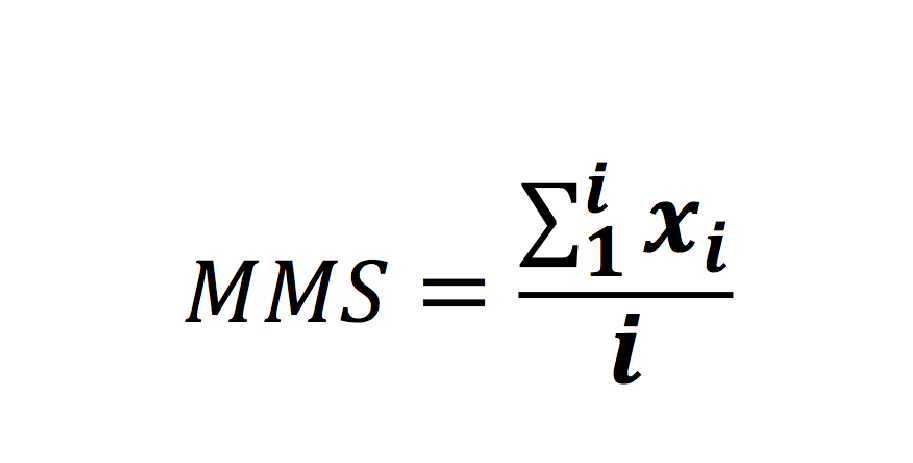
\includegraphics[width=0.8\textwidth]{figuras/f22}
\caption{Média Móvel Simples}
\end{figure}


A Média Móvel Exponencial é mais ágil em relação à média simples. Ela confere peso maior aos valores mais recentes, e com isso se torna uma média mais sensível às oscilações do Mercado Financeiro.

\begin{figure}[h]
\centering
\label{f23}
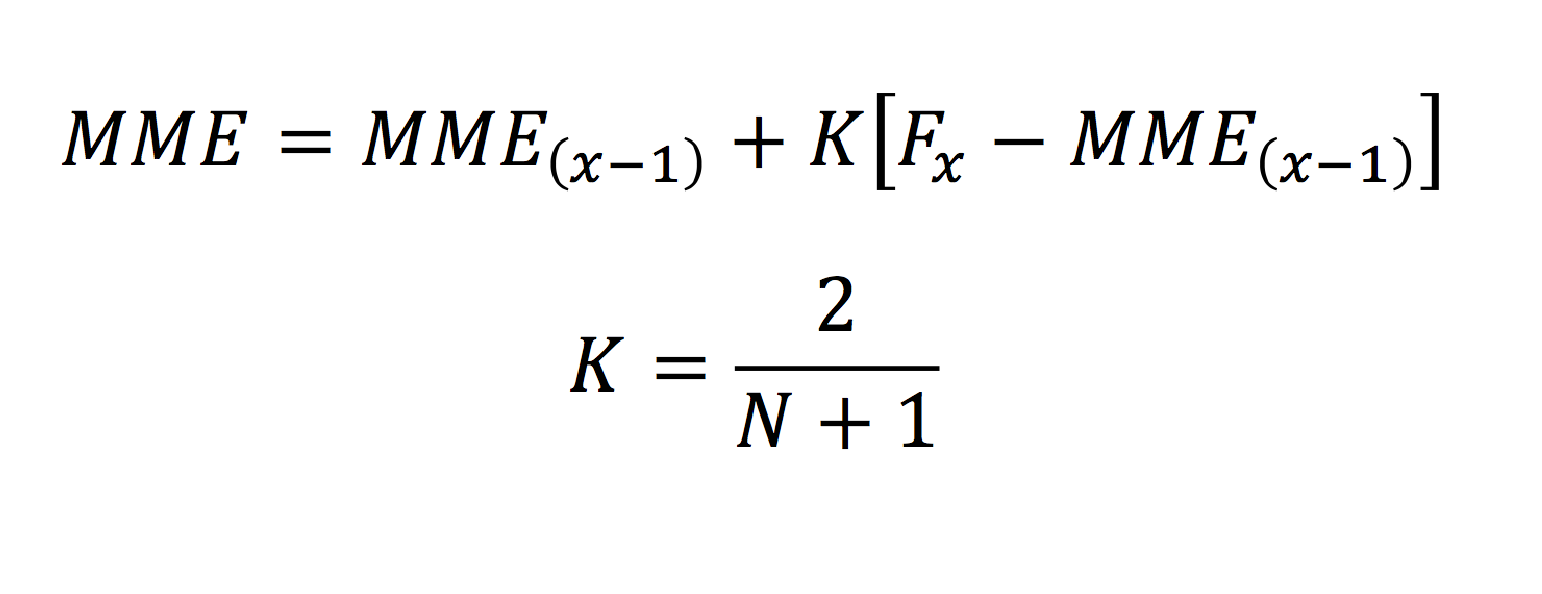
\includegraphics[width=0.8\textwidth]{figuras/f23}
\caption{Média Móvel Exponencial}
\end{figure}


Onde F é o valor de fechamento de uma ação, N é o número de períodos da média, e K é a constante calculada.

\subsection{Arquitetura MVC Aplicada à ferramenta}

Existem duas características que norteiam o desenvolvimento de um Software na atualidade, manutenabilidade e reusabilidade. Para viabilizar que a ferramenta proposta por este estudo atenda essa visão de desenvolvimento de Software, manutenível bem como reutilizável, aliado ao fato da ferramenta ser Web, o modelo arquitetural escolhido foi o MVC \cite{krasner1988}. Dessa forma, pretende-se que os códigos implementados no Paradigma de Sistemas Multiagentes possuam um alto grau de modularização, baixo acoplamento e alta coesão. Será almejado ainda possibilitar a realização de futuras manutenções de maneira mais eficiente, dado que o contexto financeiro compreende regras de negócio de alta mutabilidade. 

Em View ou Visão ,Figura 24 (\ref{f24}), concentrarão todos os códigos relacionados à interface com o usuário, seja com interfaces Web, desktop ou mobile. Esta ferramenta será construída de maneira que possa ser continuada e melhorada futuramente pelo desenvolvedor/criador ou posteriores voluntários. Em Controllerou Controle, Figura 25 \ref{f25}, concentrarão os códigos responsáveis por conectar o usuário com os agentes implementados, representando a máquina de raciocínio dos agentes - o core central do Sistema Multiagentes. Em Modelou Modelo, Figura 25 \ref{f25},concentrarão as entidades do modelo de domínio, representando os agentes de Software, outros modelos conceituais pertinentes (ex. protocolos de comunicação utilizados, regras de negócio do contexto financeiro e outros) e modelo de entidades da camada de persistência.

\begin{figure}[h]
\centering
\label{f24}
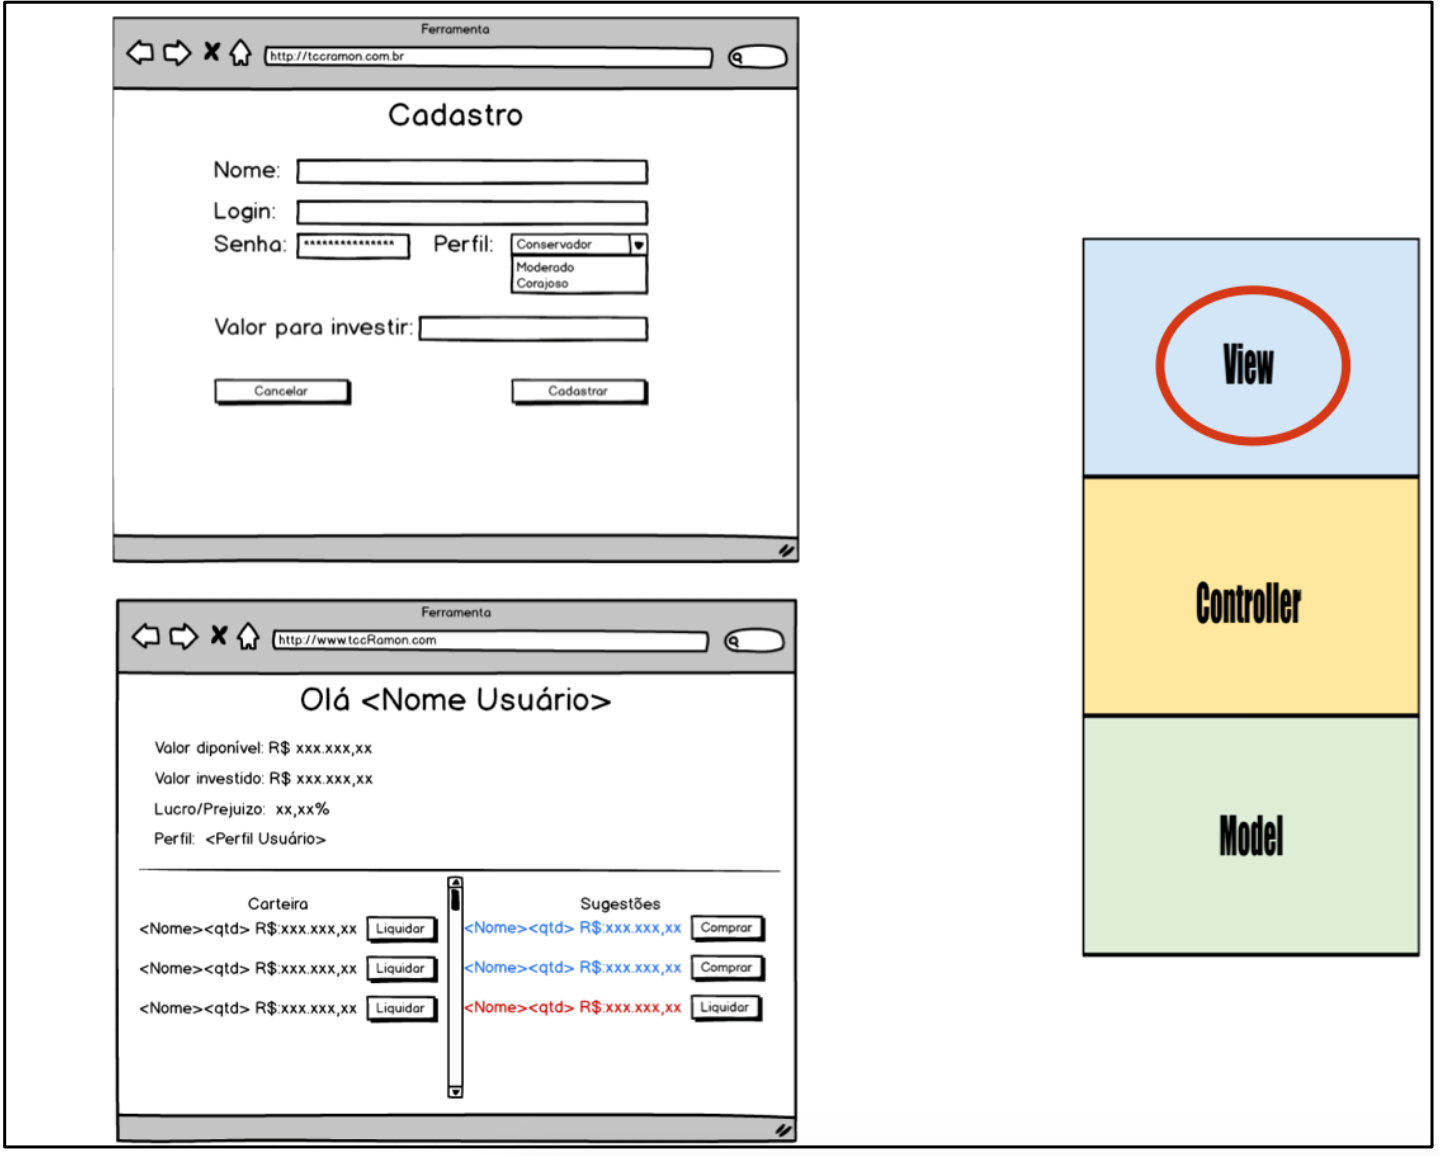
\includegraphics[width=0.8\textwidth]{figuras/f24}
\caption{Camada View}
\end{figure}

\begin{figure}[h]
\centering
\label{f25}
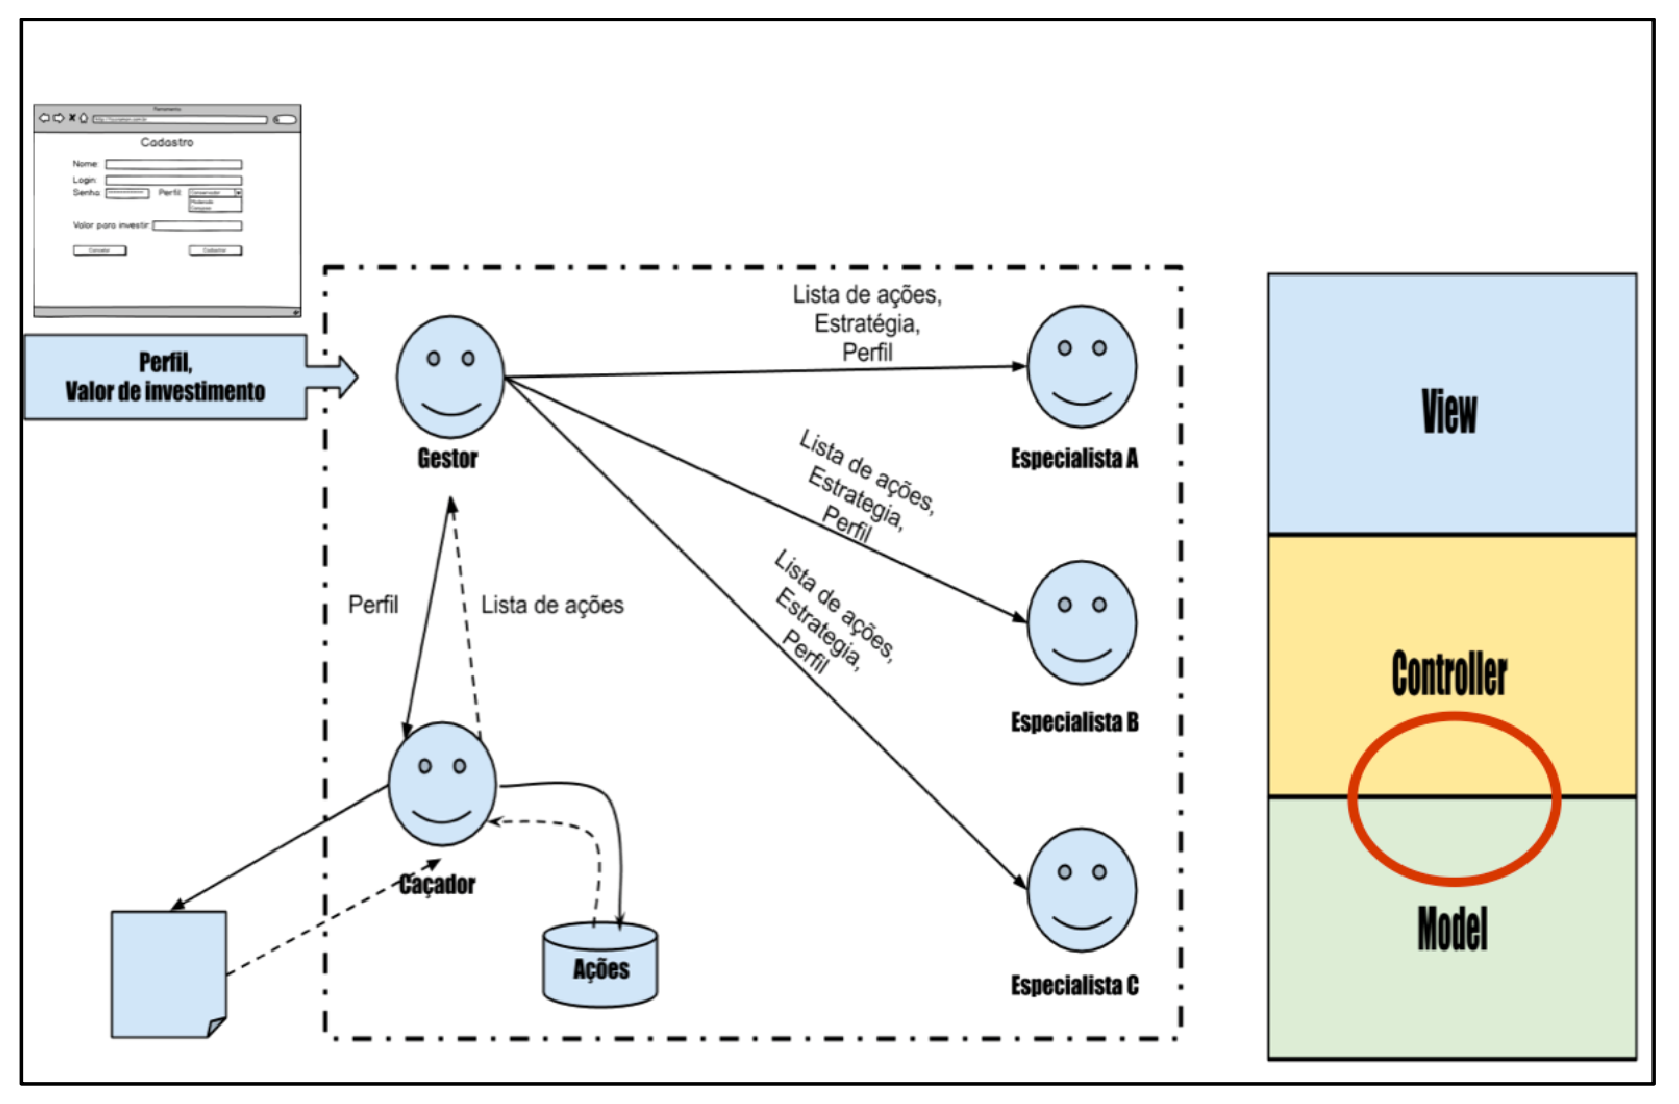
\includegraphics[width=0.8\textwidth]{figuras/f25}
\caption{Controller-Model}
\end{figure}


\section{RESUMO DO CAPÍTULO}

Este capítulo elucidou, dentre outros detalhes, uma descrição dos agentes planejados para este estudo, que serão classificados em: (i) Agente Gestor, responsável por montar equipes e gerir o risco envolvido na carteira de ações, de modo que fique alinhado com o perfil do usuário investidor; (ii) Agente Especialista, responsável por monitorar a variação dos preços das ações abordadas por ele; e (iii) o Agente Caçador, responsável por procurar ações atrativas na bolsa de valores e reportá-las aos Agentes Especialistas.

Foram apresentadas também duas estratégias financeiras, que serão implementadas neste estudo. A primeira estratégia é baseada em médias móveis. A segunda é baseada em formação de padrões em gráficos de candlesticks. Foram detalhados quatro indicadores financeiros, os quais compõem as estratégias: (i) Médias Móveis Simples e Exponencial; (ii) DarkCloud; (iii) BearishEngulfing e (iii) Bullish Engulfing.

\newpage
\chapter[METODOLOGIA DE DESENVOLVIMENTO DA FERRAMENTA]{METODOLOGIA DE DESENVOLVIMENTO DA FERRAMENTA}
\section{DESENVOLVIMENTO DO TCC}

O TCC1 foi desenvolvido considerando as seguintes atividades:
\begin{itemize}
\item Levantar Referencial Teórico:\\ Nesta atividade, foram feitos levantamentos de artigos científicos, artigos jornalísticos, publicações de empresas públicas/privadas, possíveis tecnologias que mais se alinhem à proposta, possibilitando maior conhecimento dos domínios Financeiros e de Engenharia de Software.

\item Definir escopo:\\  
Nesta atividade, o escopo do TCC foi definido como: Construir uma Ferramenta de estratégia financeira.
\item Levantar Suporte Tecnológico: \\
 Nesta atividade, foram levantadas tecnologias que mais se adequam ao proposto pelo TCC.
\item Desenvolver provas de conceito:\\ 
Nesta atividade, foram implementadas provas de conceito, utilizando uma adaptação da metodologia Scrum, em diferentes suportes tecnológicos, visando à definição de uma boa estratégia em atendimento à proposta.
\item Refinar proposta: \\
Nesta atividade, foi feita uma revisão da proposta e assim o seu refino para atividade de escrita do TCC1.
\item Escrever TCC1:\\ 
Nesta etapa foi feita a documentação dos resultados obtidos nas etapas anteriores, possibilitando a obtenção da escrita final do TCC01.
\end{itemize}

\begin{figure}[h]
\centering
\label{f26}
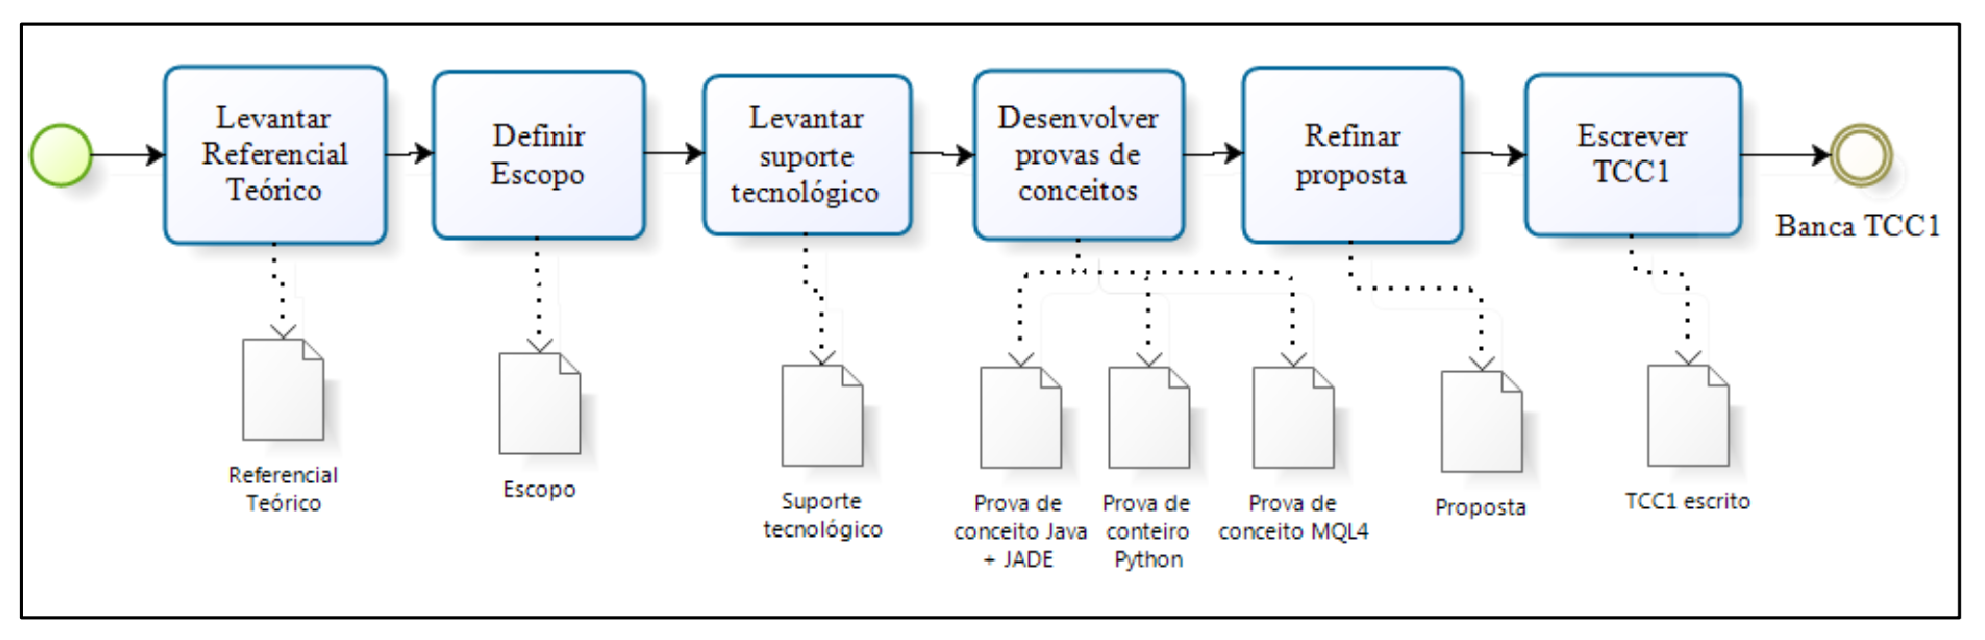
\includegraphics[width=0.8\textwidth]{figuras/f26}
\caption{Processo de desenvolvimento TCC1}
\end{figure}

Após a avaliação da Banca de TCC1, este TCC será desenvolvido considerando as seguintes atividades:

\begin{itemize}
\item Desenvolver Ferramenta:\\
Nesta atividade, será feito o desenvolvimento da Ferramenta proposta utilizando uma adaptação da metodologia Scrum. Esta atividade é descrita no subtópico 5.2.

\item Coletar impressões da ferramenta:\\
Após o desenvolvimento da ferramenta, serão coletadas as primeiras impressões da ferramenta usando como base experimentações em laboratório, possibilitando refinamentos e ajustes empíricos.

\item Escrever TCC2:\\
Nesta atividade serão feitas as subatividades: (i) Revisar e  refinar Referencial Teórico; (ii) Documentar Desenvolvimento da ferramenta; (iii) Analisar Coleta de impressões da ferramenta; (iv) Documentação do TCC2 em conformidade com as normas ABNT.

\item Escrever Artigo.
Nesta atividade, será elaborada a escrita de um artigo para publicação em eventos relacionados ao desenvolvimento de sistemas multiagentes.

\end{itemize}


\begin{figure}[h]
\centering
\label{f27}
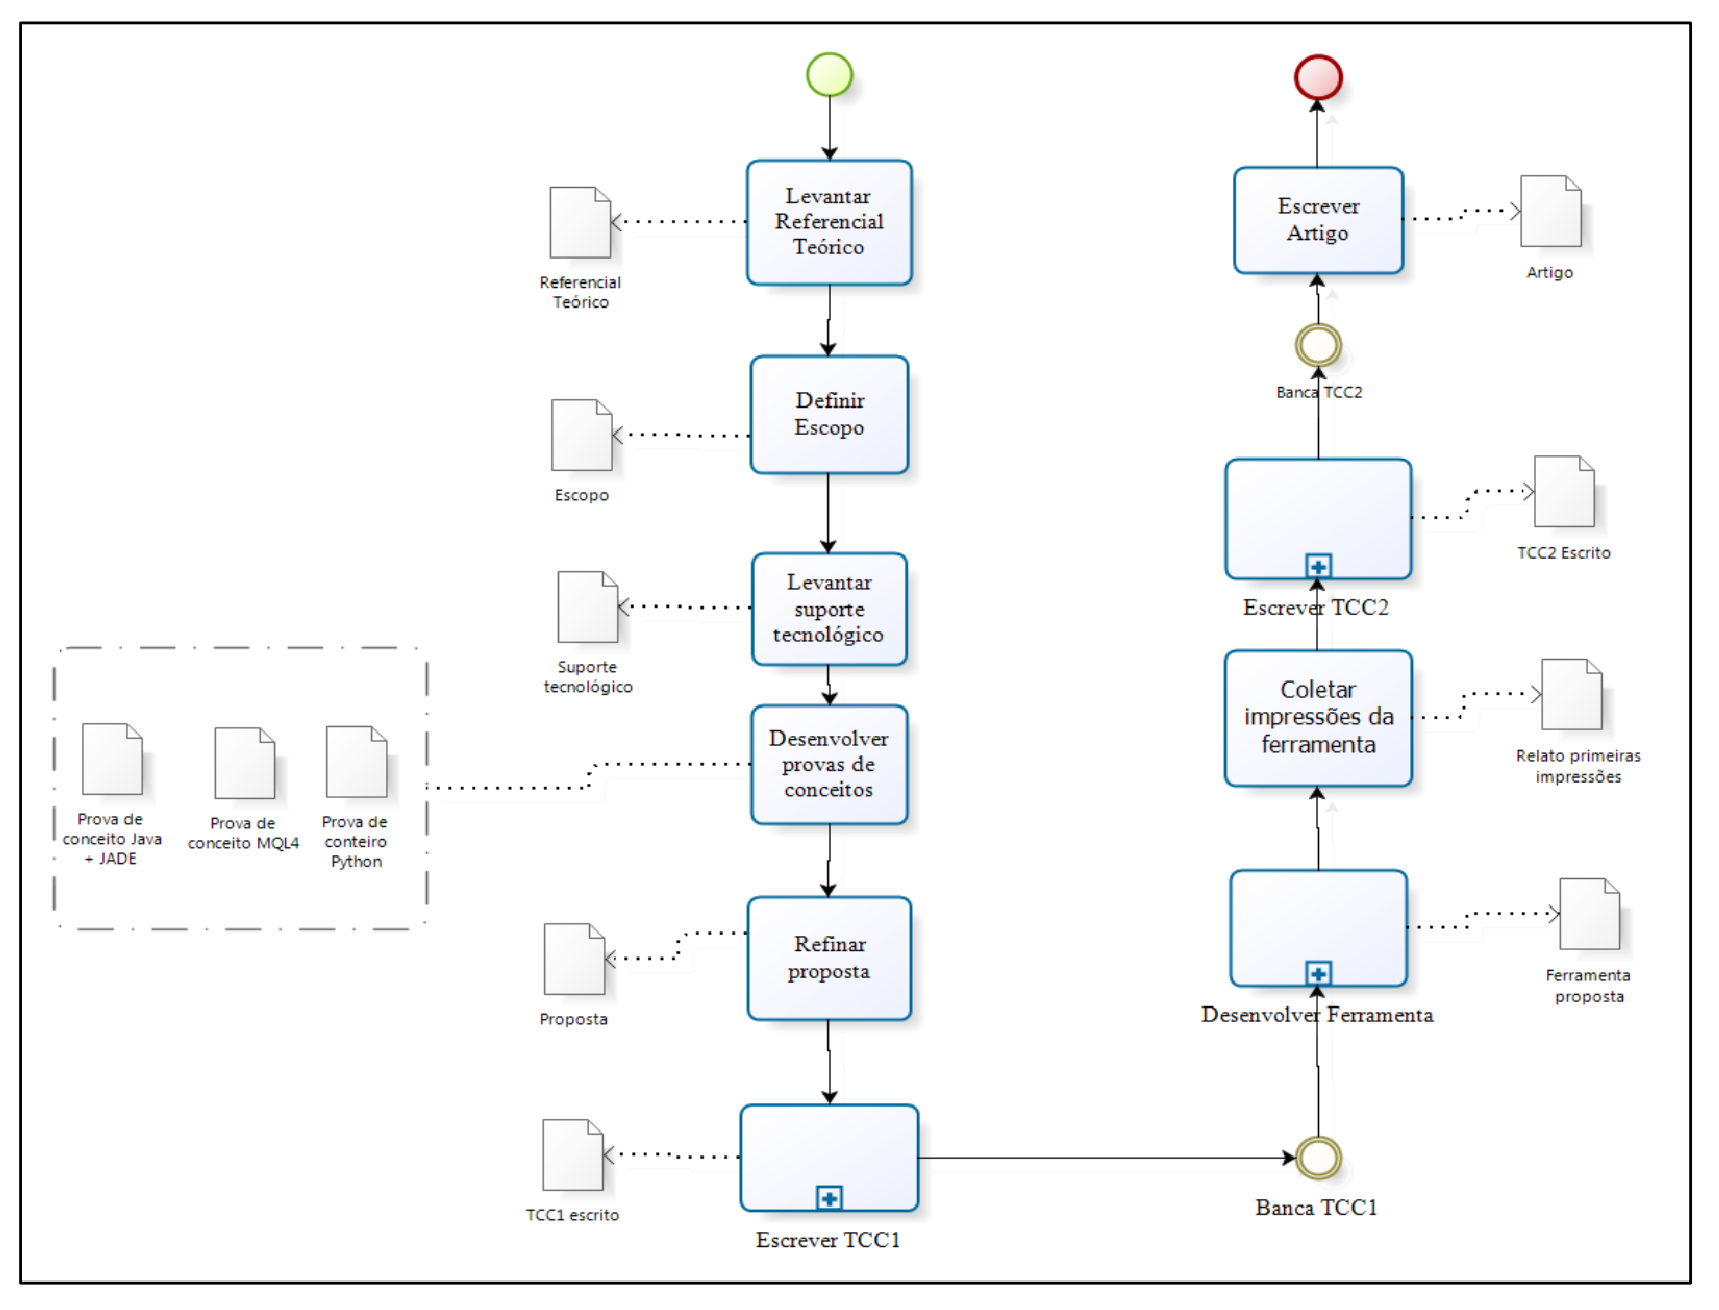
\includegraphics[width=0.8\textwidth]{figuras/f27}
\caption{Desenvolvimento TCC}
\end{figure}

\section{DESENVOLVIMENTO DA FERRAMENTA}
A ferramenta proposta neste TCC será  desenvolvida por um modelo de desenvolvimento iterativo e incremental. Para isso, foi escolhida a metodologia ágil  Scrum e foi feita uma adaptação desta, Figura 28(\ref{f28}). As estórias de usuários foram divididas em duas categorias: (i) Produto, são as funcionalidades da ferramenta proposta; e (ii) Pesquisa, são pesquisas realizadas durante as atividades de Engenharia de Software Experimental, principalmente, em relação às provas de conceito. A Tabela 5 apresenta o Productbacklog inicial deste estudo. Vale ressaltar que ele pode ser modificado durante o desenvolvimento, como previsto no Scrum.

\begin{figure}[h]
\centering
\label{f28}
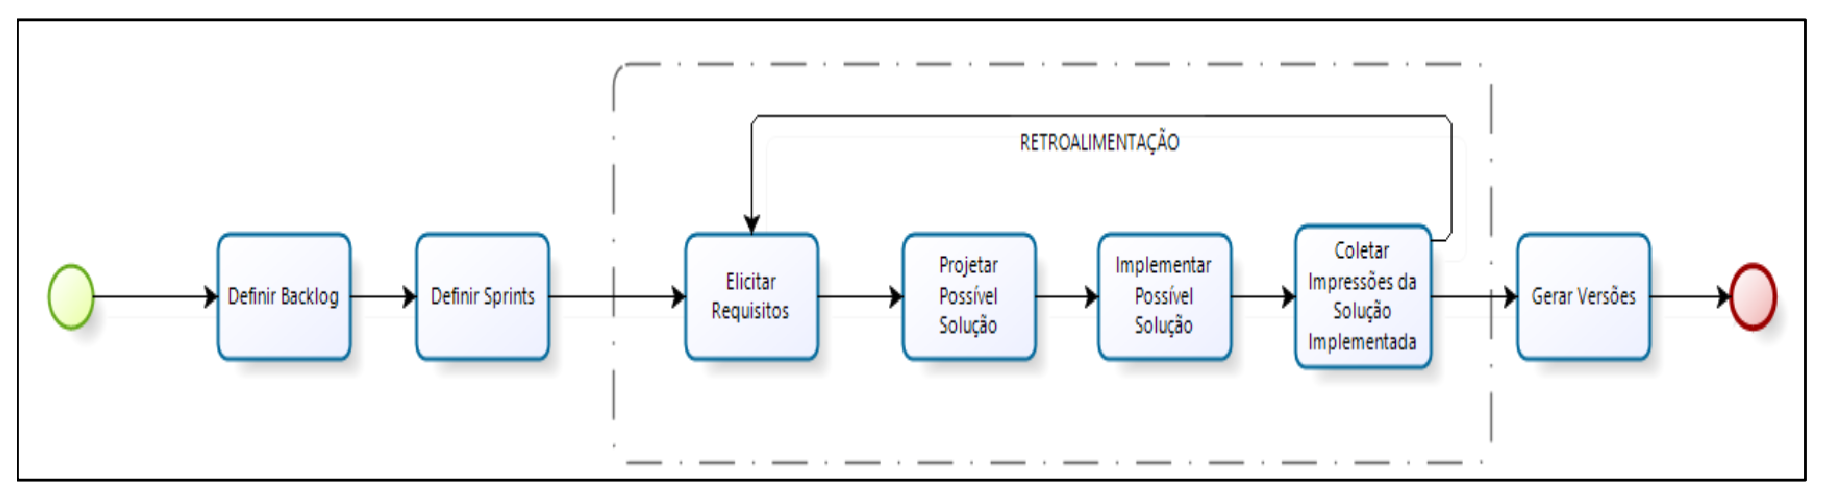
\includegraphics[width=0.8\textwidth]{figuras/f28}
\caption{Scrum adaptado para o TCC}
\end{figure}

\begin{center}
\begin{longtable}{| p{2cm} | p{10cm} |p{3cm} |}
\caption{ProductBacklog inicial} \\
\hline
\textbf{Número} & \textbf{Descrição} & \textbf{Tipo}\\\hline
\endfirsthead
\multicolumn{2}{c}%
{\tablename\ \thetable\ -- \textit{Continuação da página anterior}} \\
\hline
\textbf{Número} & \textbf{Descrição} & \textbf{Tipo}\\\hline
\endhead
\hline \multicolumn{2}{c}{\textit{Continuaçao na próxima página}} \\
\endfoot
\hline
\endlastfoot

	01 & Como engenheiro, quero um agente capaz de montar e gerir uma carteira de ações de acordo com o perfil de investidos escolhido pelo usuário e valor investido. & produto\\ \hline
	02 & Como engenheiro, quero um agente capaz de tomar estratégias financeiras de acordo com o perfil de investidor escolhido pelo usuário e valor investido. & produto\\ \hline
	03 & Como engenheiro, quero um agente capaz de realizar simulações de suas estratégias financeiras no período em que a bolsa de valores de São Paulo está fechada. & produto\\ \hline
	04 & Como engenheiro, quero um agente capaz de realizar buscas continuas de ações de empresas com presença na bolsa de valores de São Paulo e as categorize de acordo com seu setor e retorno diário. & produto\\ \hline
	05 & como engenheiro, quero um mecanismo na qual o usuário possa se cadastrar e se vincular a um grupo de agentes. & produto\\ \hline
	06 & Como engenheiro, quero um código em Python capaz de reconhecer o padrão de \textit{candlestick DarkCloud}, independentemente do ativo analisado para construir estratégias de investimentos mais eficientes. & produto\\ \hline
	07 & Como engenheiro, desejo definir estratégias de investimentos para servir de apoio aos agentes.. & produto\\ \hline
	08 & Como engenheiro, quero um código em MQL4 capaz de reconhecer o padrão de \textit{candlestick DarkCloud}, independentemente do ativo analisado para construir estratégias de investimentos mais eficientes . & produto\\ \hline
	09 & Como engenheiro, quero um código em Java+JADE capaz de reconhecer o padrão de \textit{candlestick DarkCloud}, independentemente do ativo analisado para construir estratégias de investimentos mais eficientes. & produto\\ \hline

\label{t05}
\end{longtable}
\end{center}


Nas estórias do tipo Produto, foram criadas tarefas que nortearão a implementação das estórias iniciais. Estas serão distribuídas em Sprints de 2 semanas bem como intercaladas com atividades de documentação de TCC. A seguir, encontram-se as tarefas iniciais por estória.

\begin{enumerate}
\item Eu como engenheiro, quero um agente capaz de montar e gerir uma carteira de ações de acordo com o perfil de investidos escolhido pelo usuário e valor investido.
		\begin{itemize}
		\item Implementar comunicação entre agentes gestores e caçadores;
		\item Implementar comunicação entre agentes gestores e especialistas;
		\item Implementar rotina de cálculo de riscos de carteiras para agentes gestores;
		\item Implementar critério de intervenção em operações que representem risco em desacordo com o perfil escolhido pelo usuário;
		\item Implementar rotina de criação e destruição de Agentes Especialistas;
		\item Implementar rotina de autorização de operações.
		\end{itemize}
\item Eu como engenheiro, quero um agente capaz de tomar estratégias financeiras de acordo com o perfil de investidor escolhido pelo usuário e valor investido.
		\begin{itemize}
		\item Implementar rotinas de acompanhamento de ações de empresas que compõem a carteira de investimentos;
		\item Implementar rotinas de solicitação de autorização de operações.
		\item Implementar estratégia financeira baseada em Médias Móveis;
		\item Implementar estratégia financeira baseada em Padrões de candlesticks; 
		\end{itemize}
\item Eu como engenheiro, quero um agente capaz de realizar simulações de suas estratégias financeiras no período em que a bolsa de valores de São Paulo está fechada;
		\begin{itemize}
		\item Implementar rotina de simulação de estratégias em dados históricos;
		\item Implementar rotina de persistência de resultados obtidos.
		\end{itemize}
\item Eu como engenheiro, quero um agente capaz de realizar buscas continuas de ações de empresas com presença na bolsa de valores de São Paulo e as categorizar de acordo com seu setor e retorno diário.
		\begin{itemize}
		\item Implementar rotinas de busca de ações na bolsa de São Paulo;
		\item Implementar rotinas de triagem e persistência de ações;
		\item Implementar rotinas de criação de Agentes Caçadores.
		\end{itemize}

\item Eu como engenheiro, quero um mecanismo no qual o usuário possa se cadastrar e se vincular a um grupo de agentes.
		\begin{itemize}
		\item Implementar interface com o usuário e rotina de login;
		\item Implementar rotina de instanciação de Agentes Gestores.
		\end{itemize}

\end{enumerate}

\section{ESTADO ATUAL}
\subsection{Contexto Financeiro}

O levantamento conceitual foi feito através da leitura de livros especializados em técnicas de análise financeira, os quais o autor leu no decorrer de 4 anos. Dentre os livros especializados, encontram-se: Operações lucrativas com Candlestick- Identificando Oportunidades de Mercado para Maximizar os Lucros, escrito por Stephen W. Bigalow; (ii) É só isso?! - Essência de 40 anos de estudos e práticas de análise técnica em 292 páginas, escrito por Marcio Noronha; (iii) Comprar ou Vender: Como Investir na Bolsa de Valores Utilizando Análise Gráfica, escrito por Eduardo Matsura; (iv) Como ganhar dinheiro no Mercado Financeiro - Encontre o perfil de investidor adequado à sua personalidade, escrito por Rafael Paschoarelli; e (v) Investimentos - Como Administrar melhor o seu dinheiro, escrito por Mauro Halfeld. Os livros mencionados totalizam em torno de 1.000 páginas lidas, além de várias horas de vídeos de especialistas de mercado e participação em minicursos oferecidos pela corretora XP Investimentos.

\subsection{Desenvolvimento da Ferramenta}
Foi feita uma medição do percentual de implementação com base nas funcionalidades planejadas, provindas das estórias de usuário, tanto do tipo Produto quanto do tipo Pesquisa, mencionadas no capítulo anterior. As tabelas de 6 a 8, a seguir apresentadas, reportam os percentuais calculados.


\begin{center}
\begin{longtable}{| p{2cm} | p{8cm} |p{2cm} |}
\caption{Tarefas concluídas} \\
\hline
\textbf{Estória} & \textbf{Tarefa} & \textbf{Percentual}\\ \hline
\endfirsthead
\multicolumn{2}{c}%
{\tablename\ \thetable\ -- \textit{Continuação da página anterior}} \\
\hline
\textbf{Estória} & \textbf{Tarefa} & \textbf{Percentual}\\ \hline
\endhead
\hline \multicolumn{2}{c}{\textit{Continuaçao na próxima página}} \\
\endfoot
\hline
\endlastfoot

	{} & Implementar comunicação entre Agentes Gestores e Caçadores; & \% \\ \cline{2-3}
	{} & Implementar comunicação entre Agentes Gestores e Especialistas; & \% \\ \cline{2-3}
	{} & Implementar rotina de calculo de riscos de carteiras para Agentes Gestores; & \% \\ \cline{2-3}
	01 & Implementar critério de intervenção em operações que representem risco em desacordo com o perfil escolhido pelo usuário; & \% \\ \cline{2-3}
	{} & Implementar rotina de criação e destruição de Agentes Especialistas; & \% \\ \cline{2-3}
	{} & Implementar rotina de autorização de operações; & \% \\ \hline

	{} & Implementar rotinas de acompanhamento de ações de empresas que compõem a carteira de investimentos; & \% \\ \cline{2-3}
	{} & Implementar rotinas de solicitação de autorização de operações; & \% \\ \cline{2-3}
	02 & Implementar estratégia financeira baseada em Médias Móveis; & \% \\ \cline{2-3}
	{} & Implementar estratégia financeira padrões de \textit{candlesticks}; & \% \\ \hline

	03 & Implementar rotina de simulação de estratégias em dados históricos; & \% \\ \cline{2-3}
	{} & Implementar rotina de persistência de resultados obtidos; & \% \\ \hline

	{} & Implementar rotinas de busca de ações na bolsa de São Paulo; & \% \\ \cline{2-3}
	04 & Implementar rotinas de triagem e persistência de ações; & \% \\ \cline{2-3}
	{} & Implementar rotinas de criação de Agentes Caçadores; & \% \\ \hline

	05 & Implementar interface com o usuário e rotina de login; & \% \\ \cline{2-3}
	{} & Implementar rotina de instanciação de Agentes Gestores; & \% \\ \hline
	{} & Total & \% \\ 
	
\label{t06}
\end{longtable}
\end{center}


\begin{center}
\begin{longtable}{| p{2cm} | p{8cm} | p{2cm} |}
\caption{Percentual de estórias de pesquisas concluídas} \\
\hline
\textbf{Número} & \textbf{Descrição}  & \textbf{Percentual}\\ \hline
\endfirsthead
\multicolumn{2}{c}%
{
\tablename\ \thetable\ -- \textit{Continuação da página anterior}} \\
\hline
\textbf{Número} & \textbf{Descrição}  & \textbf{Percentual}\\ \hline
\endhead
\hline \multicolumn{2}{c}{\textit{Continuaçao na próxima página}} \\
\endfoot
\hline
\endlastfoot
	06 & Eu, como pesquisador, quero um código em Python capaz de reconhecer o padrão de \textit{candlestick DarkCloud}, independentemente do ativo analisado para construir estratégias de investimentos mais eficientes & \% \\ \hline
	07 & Eu, como pesquisador, desejo definir estratégias de investimentos de curto prazo em um agente visando testar sua capacidade em atuar no mercado; & \%\\ \hline
	08 & Eu, como pesquisador, quero um código em MQL4 capaz de reconhecer o padrão de \textit{candlestick DarkCloud}, independentemente do ativo analisado para construir estratégias de investimentos mais eficientes; & \%\\ \hline
	09 & Eu, como pesquisador, quero um código em Java+ JADE capaz de reconhecer o padrão de \textit{candlestick DarkCloud}, independentemente do ativo analisado para construir estratégias de investimentos mais eficientes. & \%\\ \hline
	{} & Total Concluído. & \%\\ \hline
\label{t07}
\end{longtable}
\end{center}


\begin{center}
\begin{longtable}{| p{5cm} | p{6cm} |p{5cm} |}
\caption{Percentual Geral de conclusão da Ferramenta} \\
\hline
\textbf{Item} & \textbf{Percentual do item}  & \textbf{Percentual Relativo}\\ \hline
\endfirsthead
\multicolumn{2}{c}%
{\tablename\ \thetable\ -- \textit{Continuação da página anterior}} \\
\hline
\textbf{Item} & \textbf{Percentual do item}  & \textbf{Percentual Relativo}\\ \hline
\endhead
\hline \multicolumn{2}{c}{\textit{Continuaçao na próxima página}} \\
\endfoot
\hline
\endlastfoot
	Estória de produto & \% .& \% de 80\%\\ \hline
	Estória de pesquisa & 100\% & 100\% de 20\%.\\\hline
	{} & Total Geral & \%
\label{t08}
\end{longtable}
\end{center}


\section{RESUMO DO CAPÍTULO}
Foi exposto o modelo de desenvolvimento de Software adotado. Este, iterativo e incremental, com a adaptação da metodologia ágil Scrum, bem como uma visão geral desta metodologia. Foi apresentado também o ProductBacklog inicial com suas respectivas tarefas,planejado para este estudo. As literaturas específicas lidas no decorrer de 4 anos de estudos no contexto financeiro. E os percentuais de conclusão deste estudo, onde têm-se: (i) Implementação deEstórias de Produto, 5,8\%; (ii) Implementação de estórias de pesquisa , 100\%.Totalizando23,9\% de conclusão deste estudo.


\newpage
\chapter{RESULTADOS}
\section{AGENTES IMPLEMENTADOS}

Conforme proposto no capítulo 4, Foram implementados os 3 tipos de agentes de Software planejados: (i) Agente Gestor; (ii) Agente Especialista; (iii) Agente Caçador. No entanto, identificou-se a necessidade em criar um quarto tipo de Agente de Software, o Agente Criador. Este responsável por auxiliar na comunicação entre usuários web com seus respectivos Agentes de Software. Este Agente e os demais estão descritos nos tópicos abaixo.

\subsection{Agente Gestor}

Conforme descrito no capitulo 4 tópico 4.2.1.1, o Agente do tipo Gestor é o responsável por administrar a carteira de ações dos usuários, ações que por sua vez são acompanhadas por Agentes Especialistas. Ele autoriza uma compra ou venda de ações analisadas pelos Agentes Especialistas, vale ressaltar que essa autorização passa pelo usuário vinculado ao grupo de Agentes. O Agente Gestor, de maneira autônoma, faz o monitoramento de risco envolvido na carteira de ações administrada. Bem como, executa o processo de montagem de carteira de maneira alinhada com o perfil escolhido pelo usuário. De acordo com as responsabilidades descritas no capitulo 4 tópicos 4.2.1.1 e 4.2.2, foram implementadas as seguintes responsabilidades: 

\subsubsection{Criar e excluir um ou mais Agentes Especialistas}

Todo Agente Gestor é criado pelo Agente Criador presente no servidor (Agente descrito no tópico 6.1.4). A figura 29 ilustra o processo de criação dos Agentes especialistas de acordo com o perfil escolhido pelo usuário, e a figura 30 apresenta o trecho de código Java que implementa o processo de criação dos Agentes Especialistas.  Após criados os Especialistas, é iniciado o processo de montagem de carteira de ações. Apresentado no tópico seguinte.

\begin{figure}[h]
\centering
\label{f29}
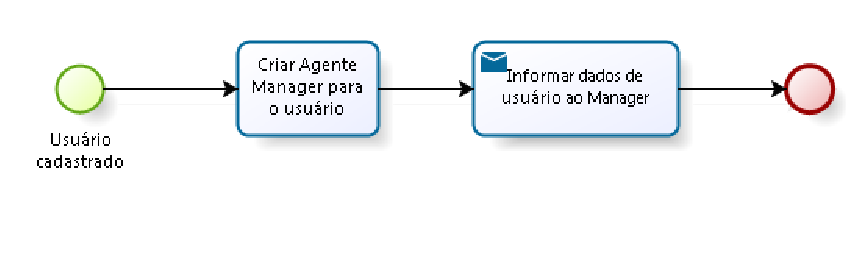
\includegraphics[width=0.9\textwidth]{figuras/f29}
\caption{Processo de criação dos Agentes do tipo Gestor }
\end{figure}

\begin{figure}[h]
\centering
\label{f30}
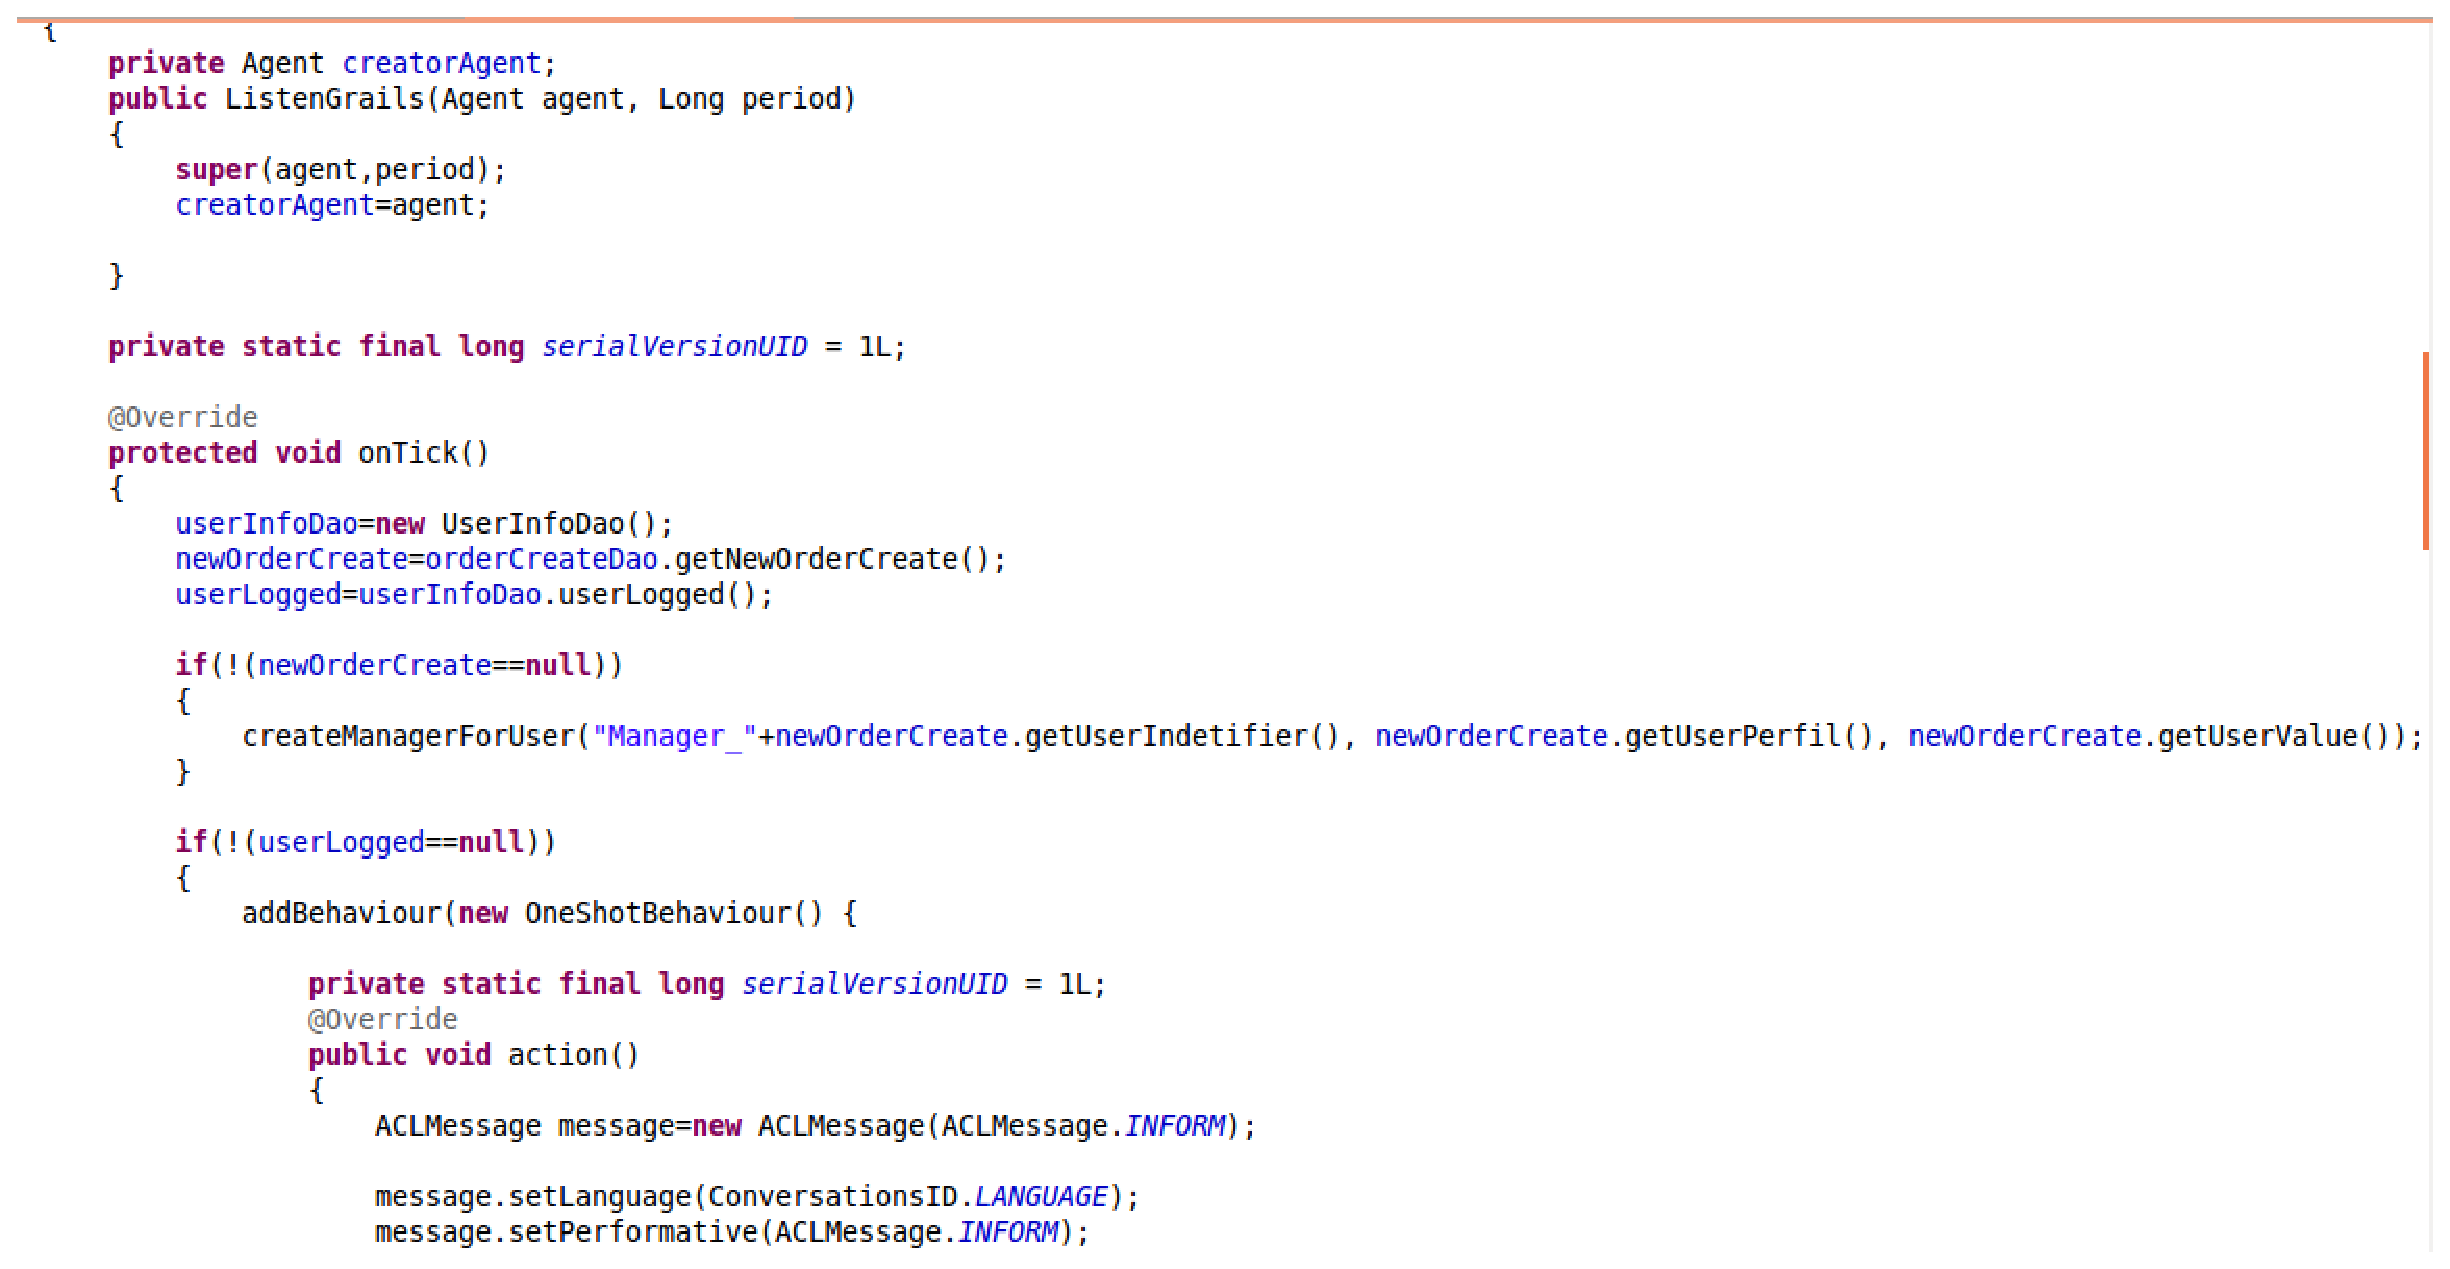
\includegraphics[width=0.9\textwidth]{figuras/f30}
\caption{Implementação Processo de Criação de Agentes do tipo Gestor}
\end{figure}

\subsubsection{Montar carteiras de ações}

A figura 31 ilustra o processo de montagem de uma carteira de ações, bem como o processo de rateio de ações entre os Agentes Especialistas vinculados ao grupo de Agentes. Vale ressaltar que de acordo com o processo previsto no capítulo 4 tópico 4.2.2.1, as ações escolhidas são alinhadas com o perfil escolhido pelo próprio usuário. O trecho de código que implementa o processo de montagem de carteira e o processo de rateio entre os Agentes Especialistas são apresentados nas figuras 32 e 33.

\begin{figure}[h]
\centering
\label{f31}
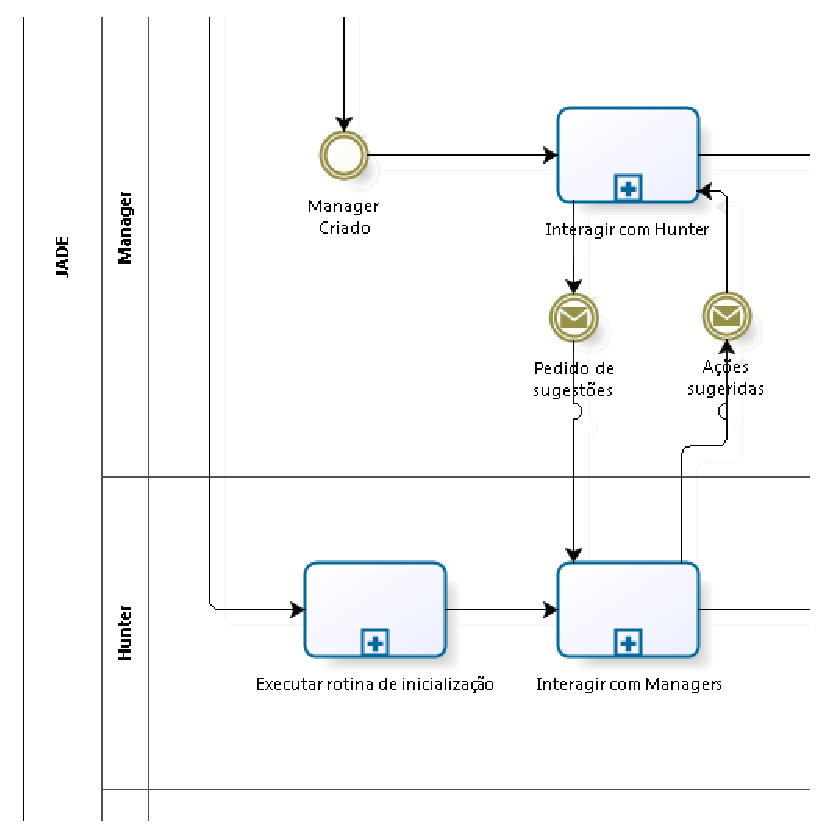
\includegraphics[width=0.9\textwidth]{figuras/f31}
\caption{Processo de montagem de uma Carteira de Ações}
\end{figure}

\begin{figure}[h]
\centering
\label{f32}
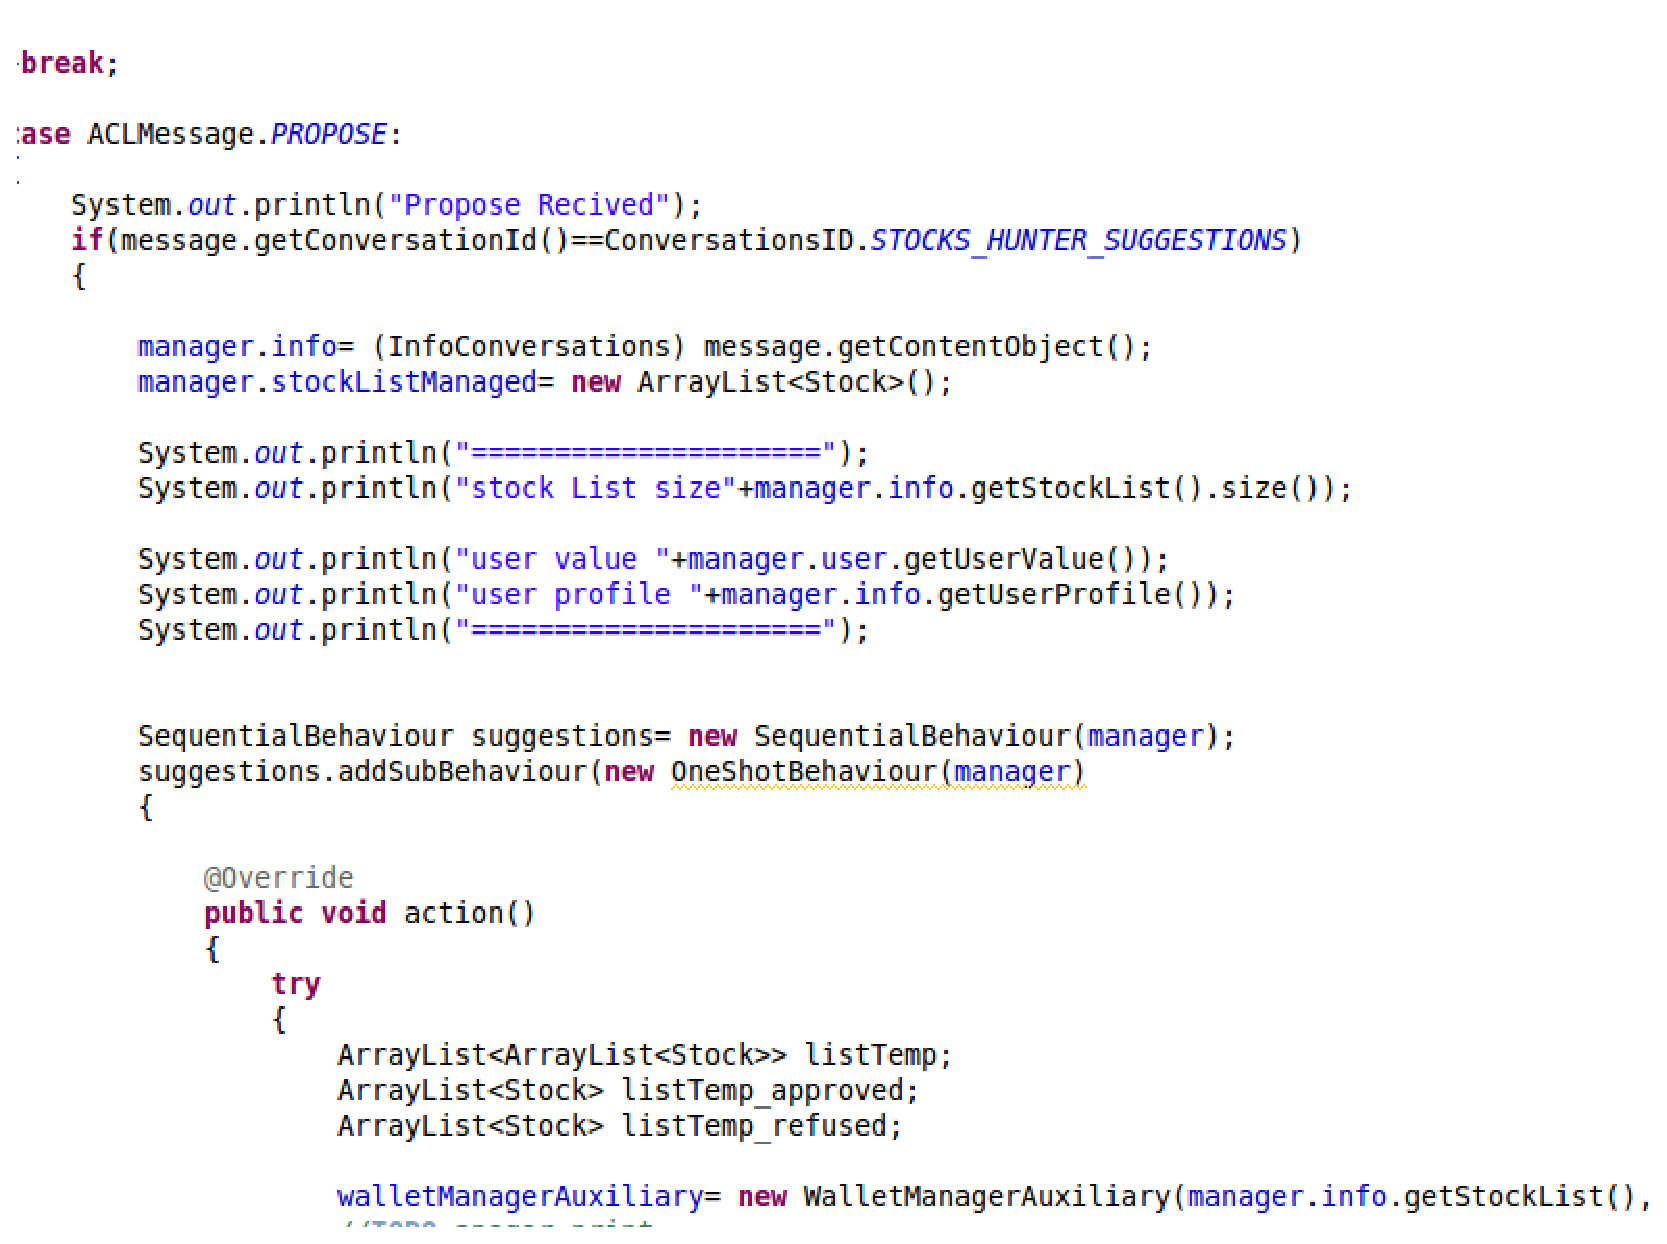
\includegraphics[width=0.9\textwidth]{figuras/f32}
\caption{Implementação processo de montagem de carteira}
\end{figure}

\begin{figure}[h]
\centering
\label{f33}
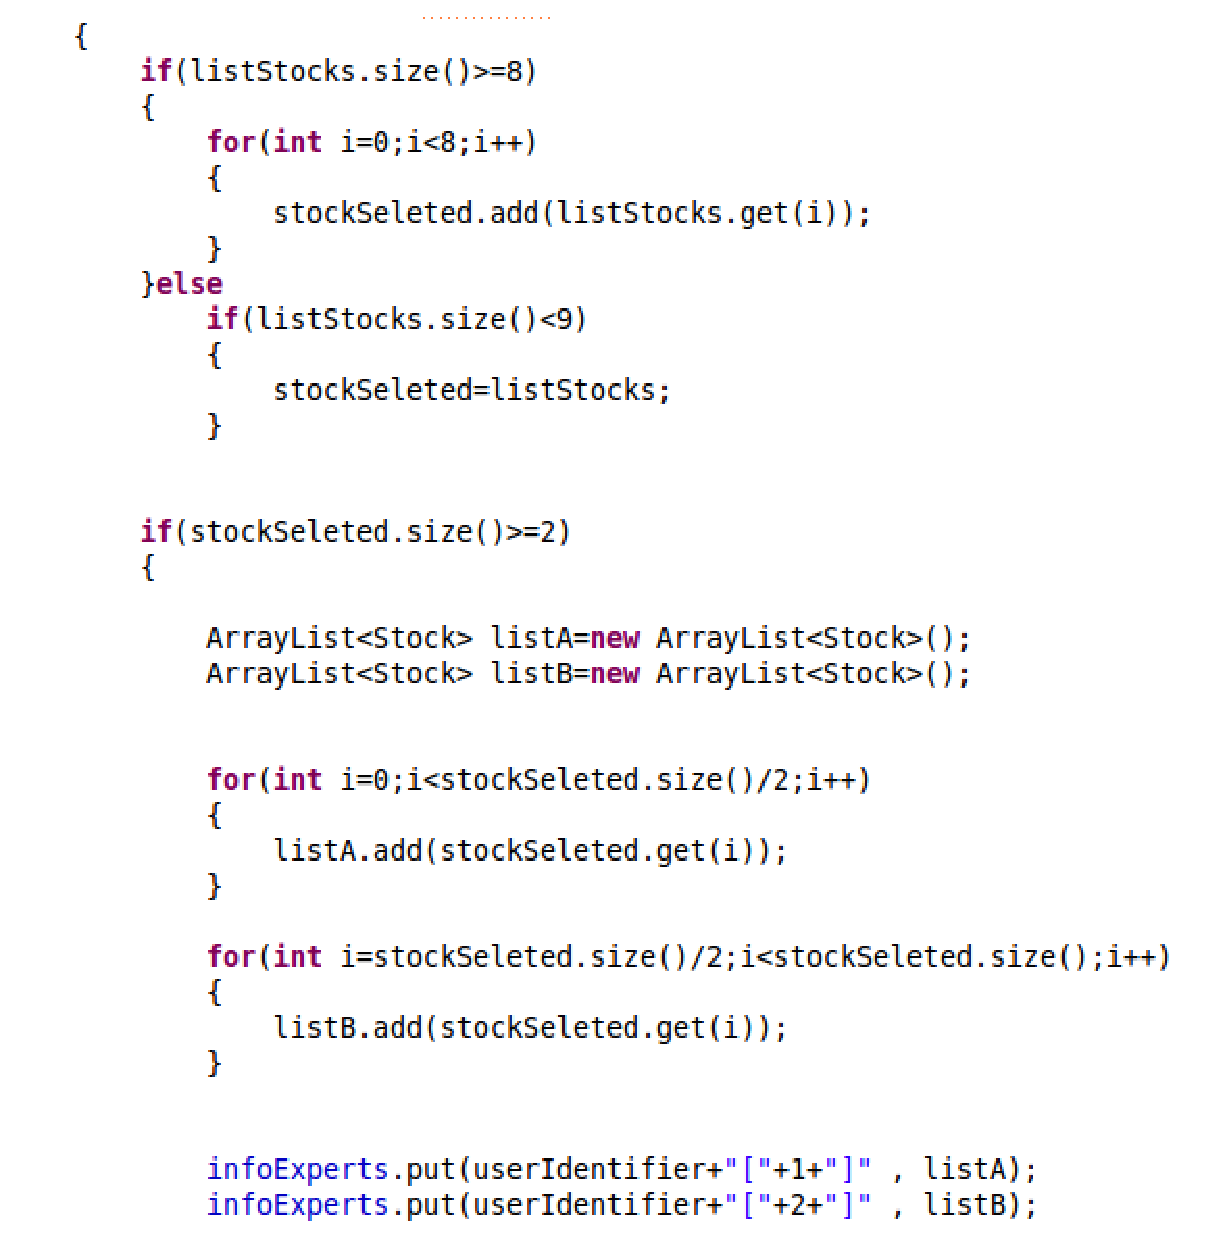
\includegraphics[width=0.5\textwidth]{figuras/f33}
\caption{Implementação processo de rateio de Ações}
\end{figure}


O processo de montagem de carteira de ações inicia-se no momento em que o um Agente Gestor é instanciado no servidor. Após ser instanciado, o Agente Gestor recebe do Agente criador uma mensagem contendo informações do usuário (Nome,Valor investido e Perfil escolhido). O Agente Gestor envia uma mensagem ao Agente Caçador de Ações instanciado no servidor solicitando um grupo de ações compatíveis ao perfil escolhido pelo usuário, figura 34. Após escolher as ações, o Agente Gestor faz o rateio entre os Agentes Especialistas, figura 35. Por fim, ao concluir os processos de montagem de carteira de ação e rateio, o Agente Gestor inicia o processo contínuo de monitoramento do risco na carteira, figura 37, conforme descrito no tópico seguinte.


\begin{figure}[h]
\centering
\label{f34}
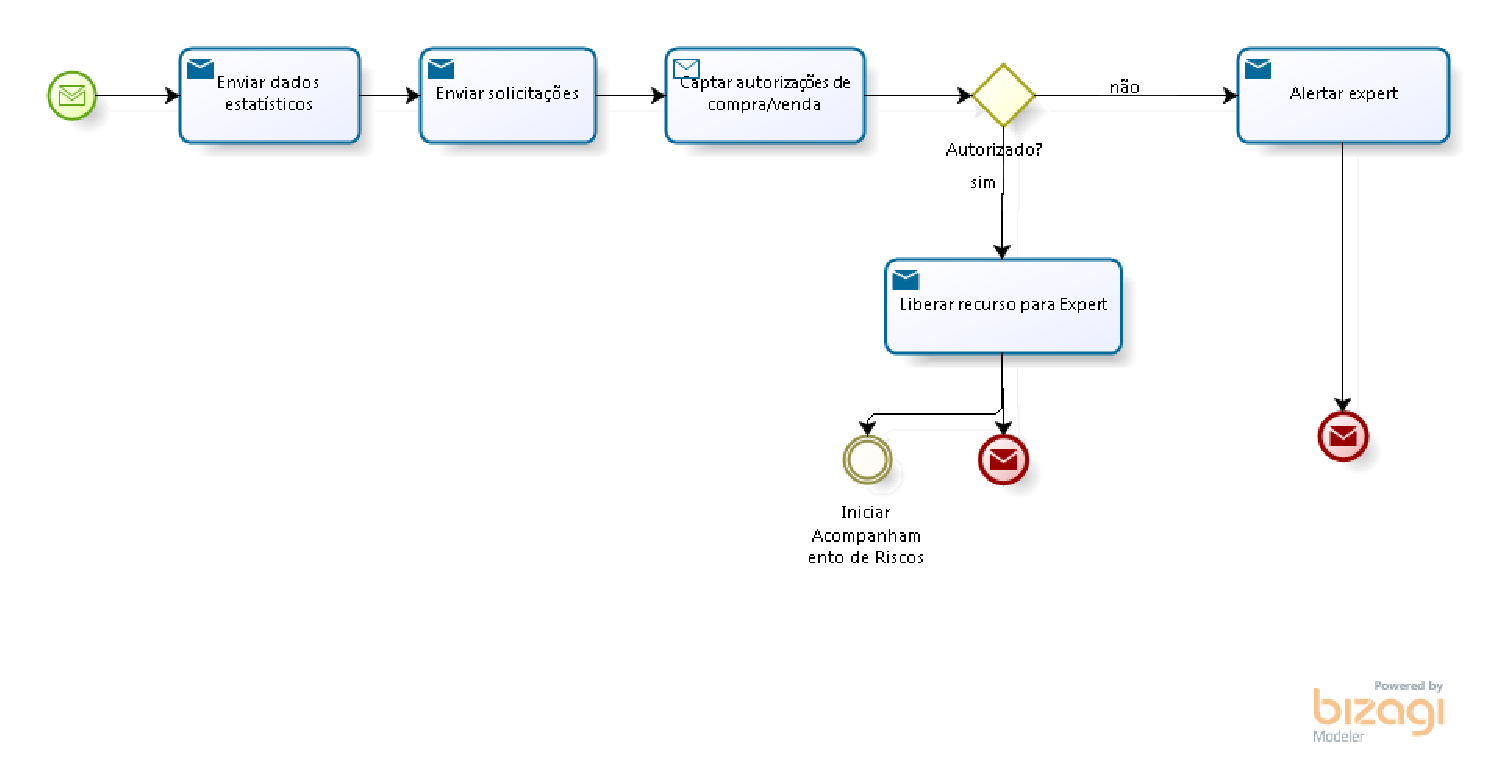
\includegraphics[width=0.5\textwidth]{figuras/f34}
\caption{Processo Troca de Mensagens Agente Gestor e Agente Criador}
\end{figure}

\begin{figure}[h]
\centering
\label{f35}
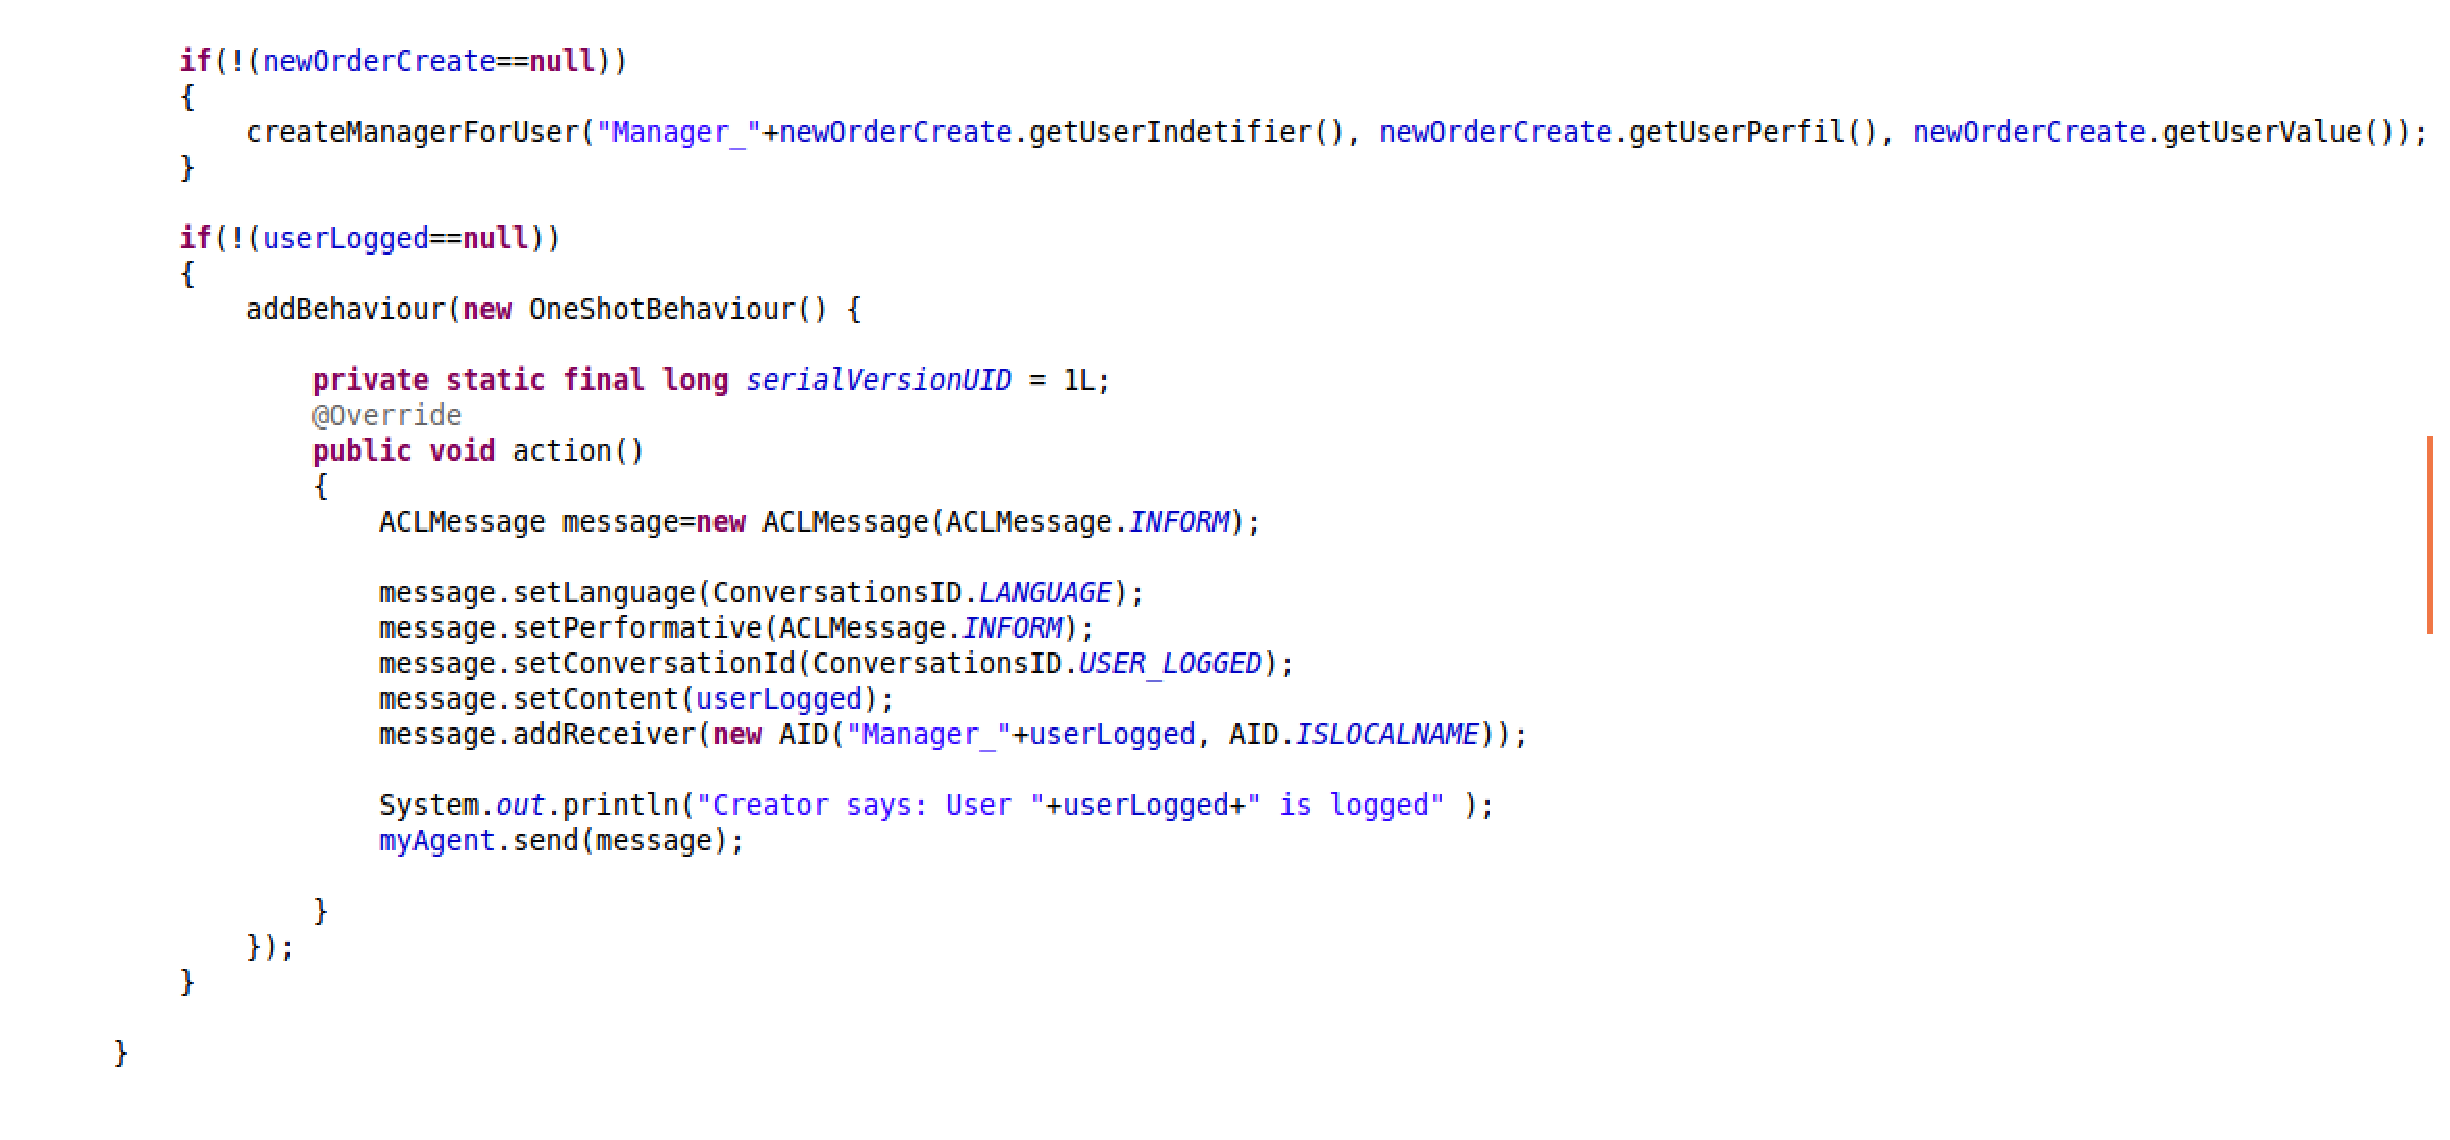
\includegraphics[width=0.5\textwidth]{figuras/f35}
\caption{Implementação Troca de Mensagens Agente Gestor e Agente Criador}
\end{figure}

\begin{figure}[h]
\centering
\label{f36}
\includegraphics[width=0.5\textwidth]{figuras/f36}
\caption{Rateio entre Agentes Especialistas}
\end{figure}

\begin{figure}[h]
\centering
\label{f37}
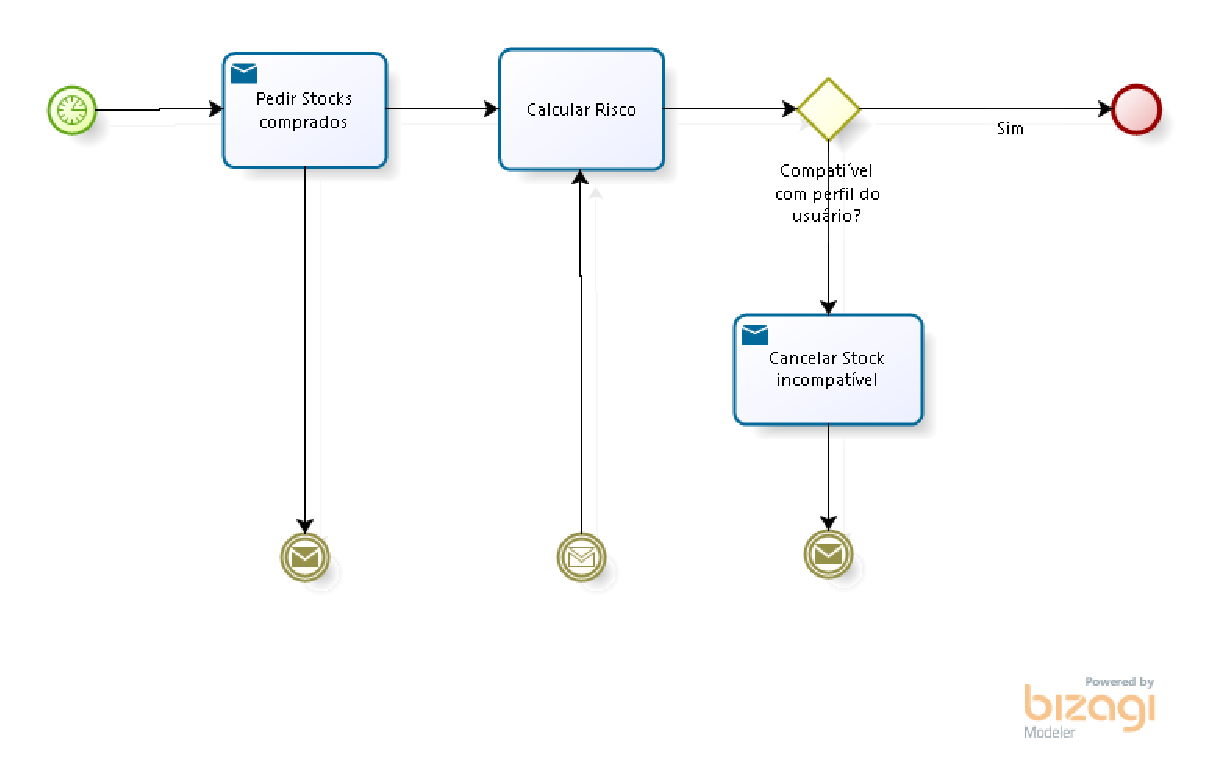
\includegraphics[width=0.5\textwidth]{figuras/f37}
\caption{Monitoramento de risco da carteira de ações}
\end{figure}

\subsubsection{Gerir careiras de ações}
Foi implementado no Agente Gestor um comportamento cíclico responsável por monitorar os riscos envolvidos na carteira de ações, que por sua vez acompanhadas por Agentes Especialistas. O Agente Gestor é capaz de cancelar uma operação de compra, caso esta represente um grau de risco incompatível com o perfil escolhido pelo usuário, figura 38.

\begin{figure}[h]
\centering
\label{f38}
\includegraphics[width=0.5\textwidth]{figuras/f38}
\caption{Acompanhamento de risco em operações}
\end{figure}

\subsection{Agente Especialista}

Conforme descrito no capítulo 4 tópico 4.2.1.2, o Agente Especialista é o Agente responsável por realizar leituras constantes do mercado de valores em busca de novas cotações das ações sob sua responsabilidade. Ele é criado pelo seu Agente Gestor e executa estratégias compatíveis com o perfil escolhido pelo usuário, recebe ainda um grupo de ações na qual será responsável. Diferente do descrito no tópico 4.2.1.2, viu se necessário transferir a responsabilidade de mensurar risco de estratégias para o seu Agente Gestor, e após implementação verificou-se empiricamente que executar uma rotina de simulação poderia onerar o servidor devido ao consumo de memória ao manipular objetos Candlesticks e grande quantidade. Com isso, foram implementadas as seguintes responsabilidades:(i) Aplicar estratégias que ofereçam o maior lucro possível compatível com o perfil escolhido pelo usuário, figura 39; e (ii) Solicitar autorização para realizar compra ou venda de ações, figura 40.

\begin{figure}[h]
\centering
\label{f39}
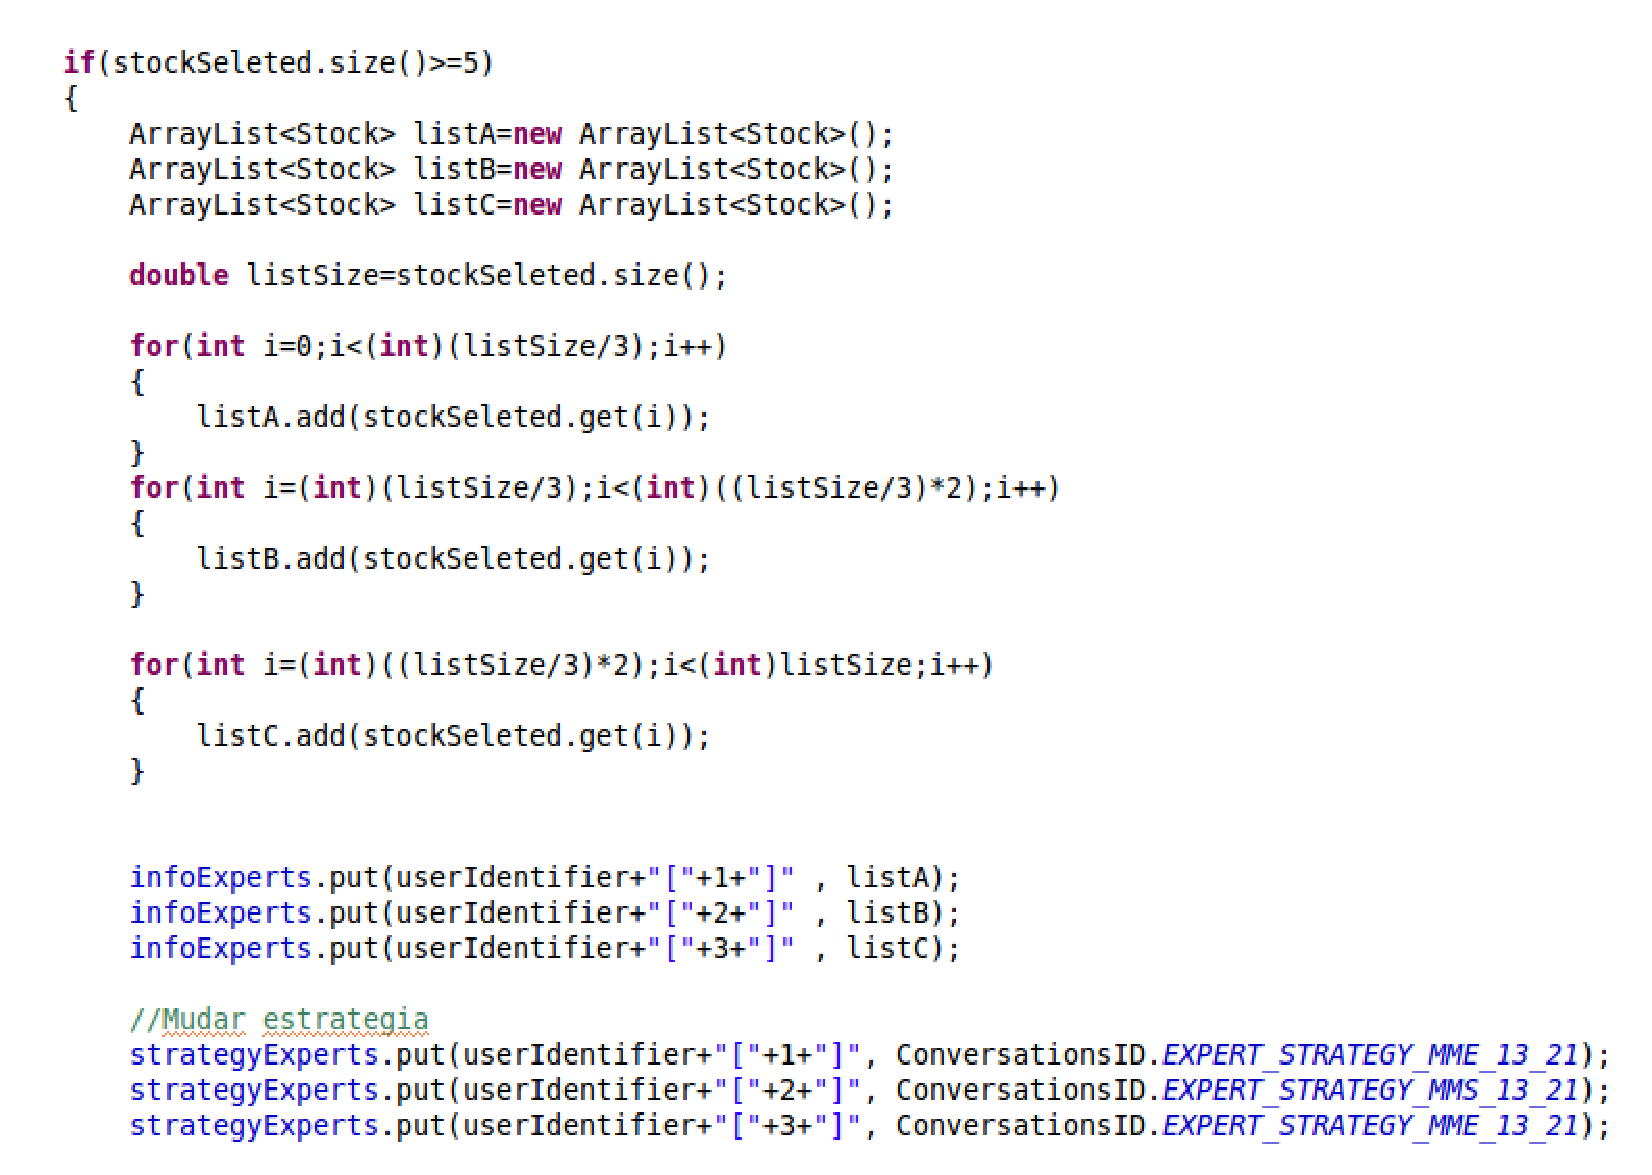
\includegraphics[width=0.5\textwidth]{figuras/f39}
\caption{Estratégias por perfil de usuário/Investidor}
\end{figure}

\begin{figure}[h]
\centering
\label{f40}
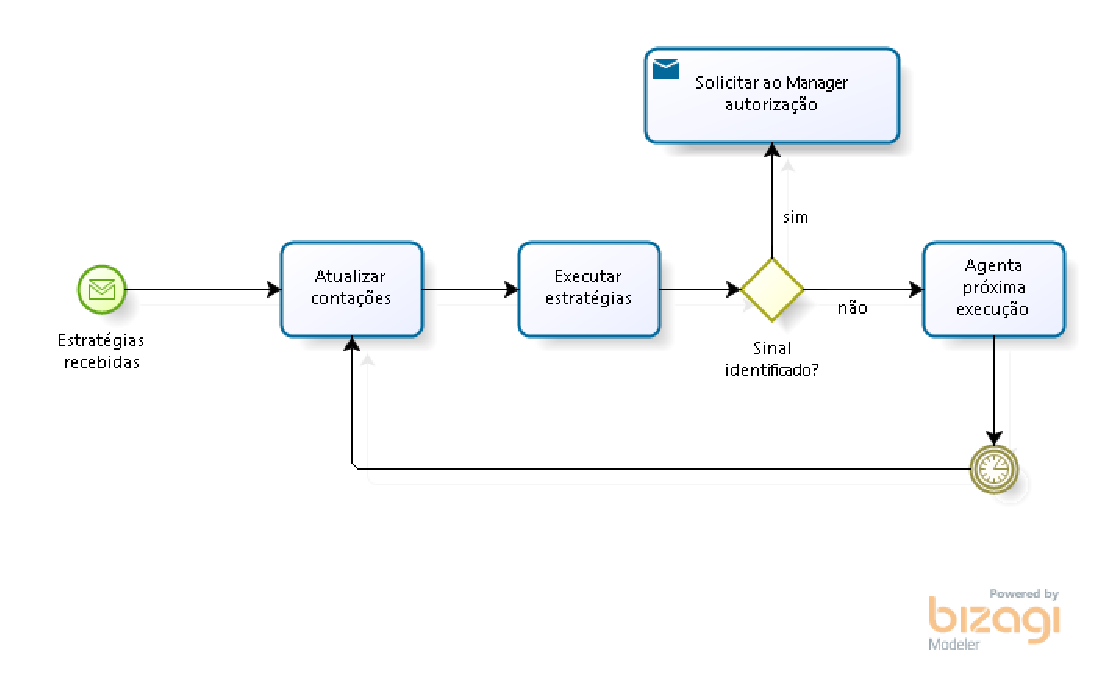
\includegraphics[width=0.5\textwidth]{figuras/f40}
\caption{Acompanhamento de risco em operações}
\end{figure}

\begin{figure}[h]
\centering
\label{f41}
\includegraphics[width=0.5\textwidth]{figuras/f41}
\caption{Implementação solicitação de autorização para realização de operação}
\end{figure}


\subsection{Agente Caçador}

Conforme descrito no capitulo 4 tópico 4.2.1.3, o Agente Caçador é responsável por fazer buscas constantes de cotações de ações presentes na bolsa de valores e trabalhadas pela ferramenta e realizará uma categorização destas ações através de valores estatísticos, tais como: (i) retorno médio diário; (ii) retorno médio 15 e 30 dias; (iii) variância média diária; e (iv) variância média 15 e 30 dias. Através destes valores, o Agente Caçador seleciona grupos de ações compatíveis com os perfis informados por Agentes Gestores no procedimento de montagem de carteira descrita no tópico 6.1.1.2. De acordo com as responsabilidades descritas no capitulo 4, foram implementadas as seguintes responsabilidades: (i) Busca e Seleção das melhores ações a se investir, estas ações variam de acordo com o perfil de usuário tratado pelos Agentes Gestores. O processo é ilustrado e sua implementação apresentada nas figuras 42 e 43, respectivamente; e (ii) categorização de ações através de valores estatísticos, o Agente caçador faz cálculos estatísticos frequentes dada ação abordada na ferramenta e os utiliza como parâmetro de escolha para selecionar ações para atender as solicitações dos Agentes Gestores, como apresentado nas figuras 43,44 e 45.

\begin{figure}[h]
\centering
\label{f42}
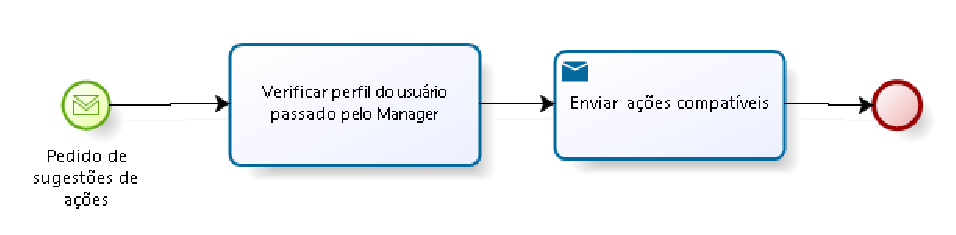
\includegraphics[width=0.5\textwidth]{figuras/f42}
\caption{Processo de escolha de ações}
\end{figure}

\begin{figure}[h]
\centering
\label{f43}
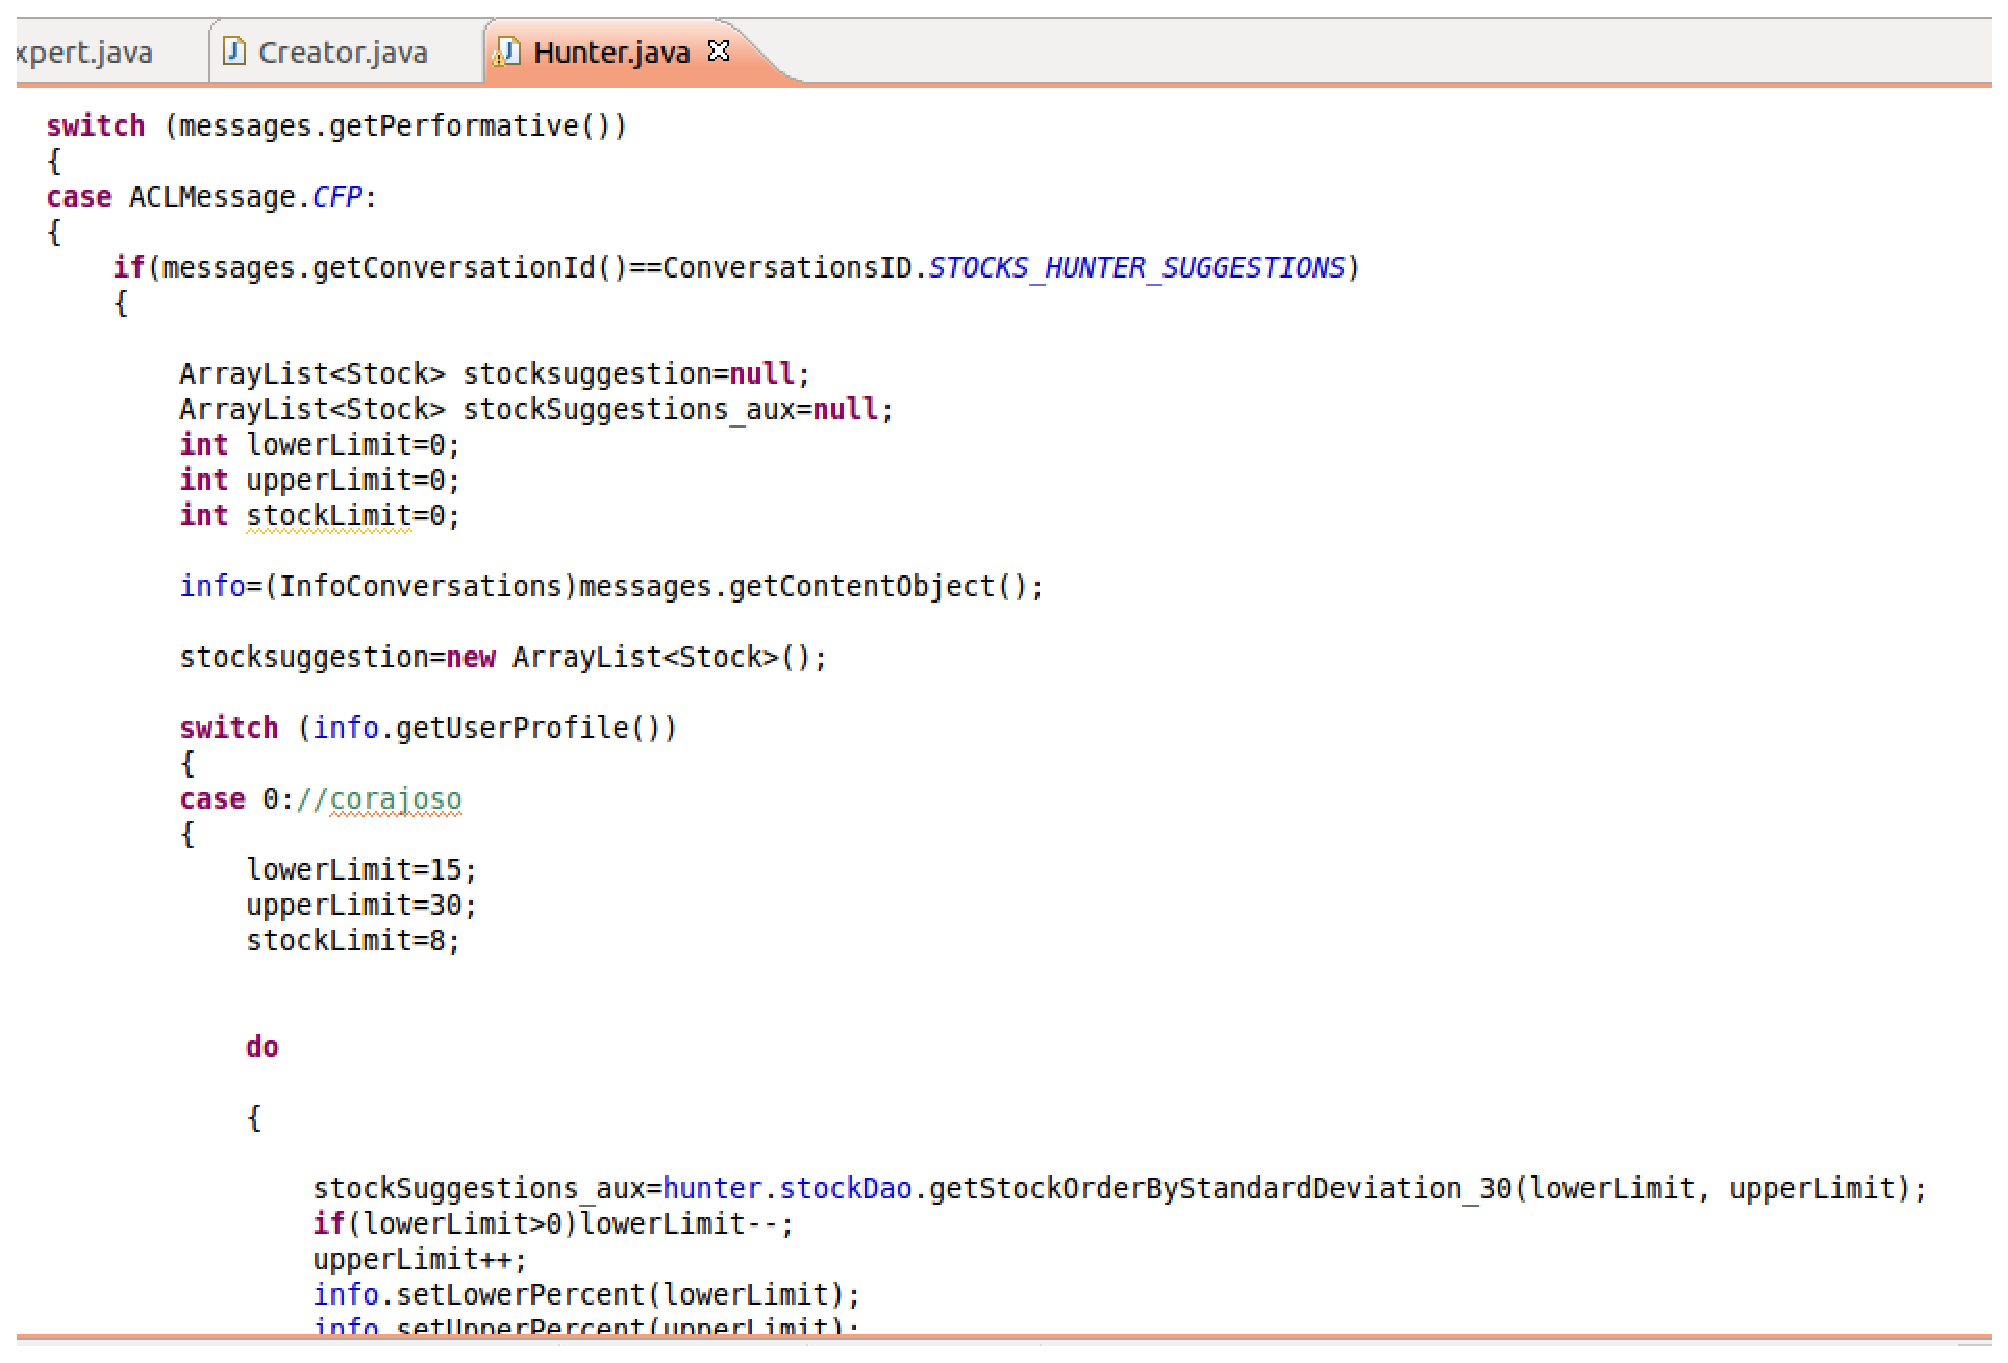
\includegraphics[width=0.5\textwidth]{figuras/f43}
\caption{Implementação processo de escolha de ações}
\end{figure}

\begin{figure}[h]
\centering
\label{f44}
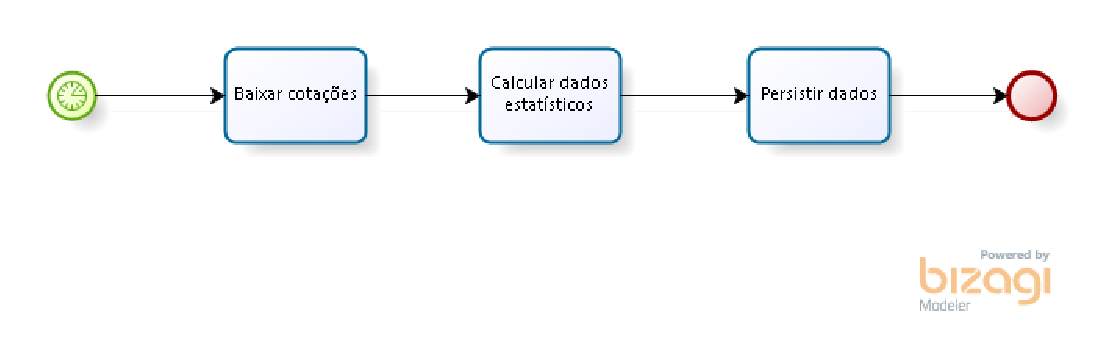
\includegraphics[width=0.5\textwidth]{figuras/f44}
\caption{Persistência de valores estatísticos por ação}
\end{figure}

\begin{figure}[h]
\centering
\label{f45}
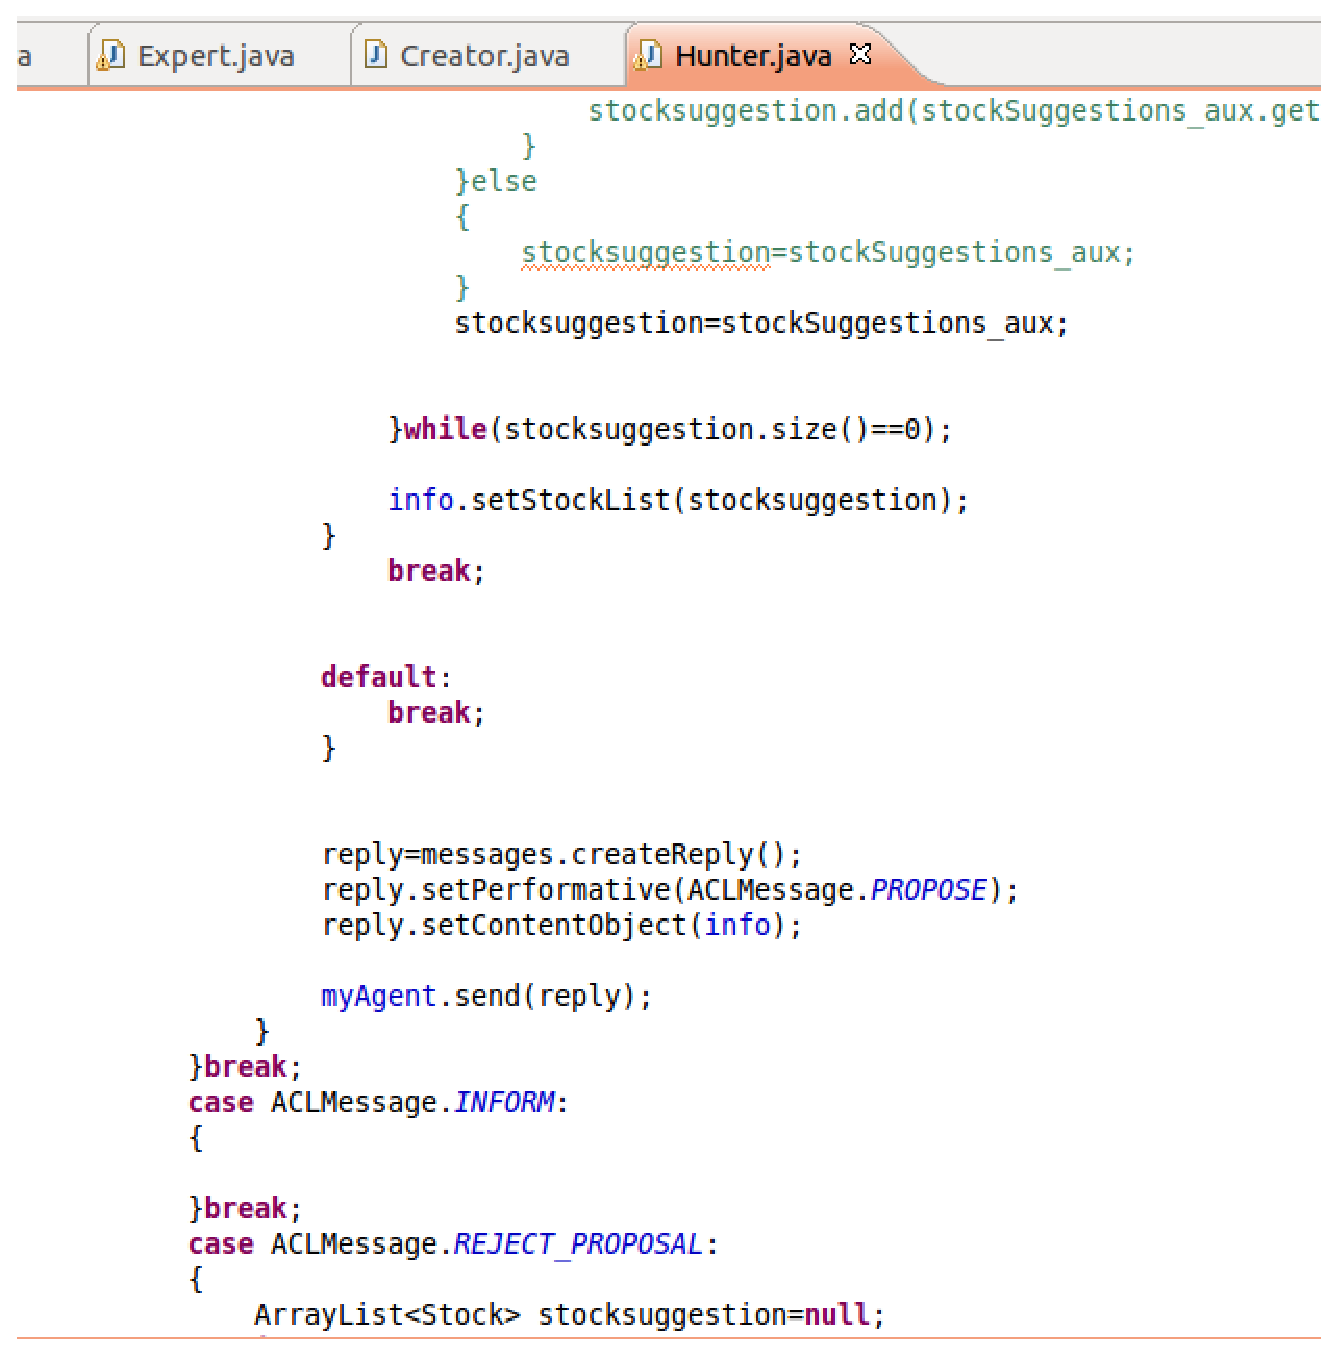
\includegraphics[width=0.5\textwidth]{figuras/f45}
\caption{Envio de grupo de ações solicitadas por um Agente Gestor}
\end{figure}

\subsection{Agente Criador}

Este agente não foi previsto no capitulo 4, porém durante a implementação verificou-se a necessário criar um tipo de Agente para auxiliar na comunicação entre os usuários e seus respectivos grupos de Agentes. Como o Agente Caçador, existe um agente Criador para cada servidor. Suas responsabilidades são: (i) Monitorar a criação de novas contas. O usuário quando cria uma conta o Agente Criador captura as informações repassadas pelo usuário, cria um Agente Gestor para este usuário e o informa através de uma mensagem com informações do usuário tais como nome, valor investido e perfil escolhido; (ii) Monitorar Log In de usuários.  Quando um usuário autentica-se na ferramenta, o Agente Criador informa ao seu Agente Gestor para que o mesmo comunique-se com seu usuário, a comunicação entre o Agente Gestor e seu respectivo usuário é demonstrado na figura 46, bem como todas funcionalidades apresentadas ao longo deste capítulo.

\textbf{Figura 46: Visão geral da ferramenta.}

\section{COLETA DE IMPRESSÕES}
\subsection{Pesquisa - Ação}
Segundo Rocha, pesquisa-ação pode ser considerada ''independente'' e ''objetiva'. E de acordo com Thiollent (1986 apud Rocha) caracteriza-se pesquisa-ação como:
\begin{citacao}
Um tipo de pesquisa social com base empírica, concebida e realizada em estreita associação com uma ação ou com a resolução de um problema coletivo no qual os pesquisadores e os participantes, representativos da situação e/ou do problema, estão envolvidos de forma cooperativa e participativa (THIOLLENT, 1986, p.3. Apud Rocha ).
\end{citacao}

A pesquisa-ação é um processo cíclico e continuo onde planeja-se, implementa-se, descreve-se e avalia-se uma mudança para a melhoria de sua prática. Desta forma há um aprendizado maior por parte do pesquisador durante o processo. Neste trabalho, o processo de pesquisa-ação foi utilizado para verificar o objetivo específico, no ponto de vista da interface com usuário: ''Abstrair a complexidade de cálculos financeiros comumente utilizados na Análise Técnica. Assim, essa complexidade não é sentida pelo usuário, deixando a mesma a cargo da ferramenta.'' apresentados no tópico XX. O cenário de uso e resultados obtidos são apresentados no tópico seguinte.


\subsection{Coleta de impressões com usuários}

Esta coleta de dados organizou-se nas seguintes etapas: (i) Planejamento, nesta etapa foram levantadas questões a serem respondidas pelos potenciais usuários de maneira a avaliar a interface gráfica da ferramenta; (ii) Implementação, nesta etapa foi elaborado um questionário a ser respondido pelos usuários, e foi montado ainda um cenário tecnológico onde a ferramenta apresentou dados em um período histórico de cotações da BM\&FBovespa ; (iii) Descrição, nesta etapa concentra-se a seguinte descrição do cenário de uso da ferramenta. A Ferramenta foi apresentada aos potenciais usuários em modo de simulação no período de 1 de março de 2013 a 1 de março de 2014, a versão do JADE utilizado é a 4.3.3 de 10 de dezembro de 2014, a versão do Grais era a 2.4.3 e a versão do java era a 1.7.0\_79. A ferramenta foi simulada ainda em um notebook da marca Apple modelo MacBook Pro (Retina, 13-inch, Late 2013) com processador 2.6 GHz Intel Core i5, com 8 GB 1600 MHz DDR3 de Memória RAM e com o Sistema operacional OS X Yosemite versão 10.10.3; (iv) Avaliação, nesta etapa foram colhidas os feedbacks dos potenciais usuários da ferramentas e foram feitas melhorias na mesma. Dentre os feedbacks recebidos destacou-se a sugestão de um usuário que se identificou com o perfil Corajoso, onde ele sugeriu usar outro indicador no lugar do indicador Média Móvel. Esta sugestão coincidiu com uma das observações obtidas ao simular as estratégias adotadas pela ferramenta, onde verificou-se que as Medias Móveis para alguns perfis não obtinham um resultado aceitável (Essas observações são expostas de maneira sucinta no tópico X e na integra no Apêndice X)

\subsubsection{Objetivos}

Esta coleta de dados com potenciais usuários teve como principal objetivo verificar  o objetivo especifico proposto: “Abstrair a complexidade de cálculos financeiros comumente utilizados na Análise Técnica. Assim, essa complexidade não é sentida pelo usuário, deixando a mesma a cargo da ferramenta”. Vale ressaltar que essa avaliação teve como foco a interface gráfica da ferramenta com os usuários, onde cada usuário recebeu um formulário com questões objetivas e um campo livre para sugestões. O comportamento dos agentes bem como os resultados das estratégias abordadas foram avaliados através de simulações, como apresentado no tópico X e apêndice X.

\subsubsection{Público alvo avaliado}

A avaliação ocorreu em maio de 2014 e participaram da avaliação 6 pessoas onde: 1 classifica-se no perfil Corajoso; 1 classifica-se no perfil Moderado e 4 classificam-se no perfil Conservador. O teste funcional da ferramenta foi feito com uso de dados históricos no período entre 1 de março de 2014 e 3 de março de 2015. Foram avaliadas neste primeiro este a interface da ferramenta.

\subsubsection{Observações colhidas}

Quando questionados sobre as cores adotadas na ferramenta, 5 pessoas consideraram boas e 1 pessoa considerou ótimas. Quando questionados sobre a facilidade de compreensão da ferramenta, 3 pessoas consideraram como bom, 1 pessoa considerou razoável, 1 pessoa considerou como ruim e 1 se absteve. Quando solicitados observações gerais para ferramenta destacaram-se: (i) feedback indicando o carregamento e o processo da ferramenta; (ii) atualizar página principal automaticamente; (iii) dispor de um canal de dúvidas; (iv) não adotar estratégias baseadas em Médias Móveis; (v) utilizar javascript na interface; (vi) Executar a ferramenta em duas máquinas; (vii) Informações sobre estratégias e uso da ferramenta.

As sugestões apresentadas pelos usuários geram demanda por melhorias na interface gráfica, como esperado, e uma demanda na melhoria nas estratégias adotadas, esta demanda coincidiu com os resultados obtidos no Relatório 02, onde verificou-se que o uso de estratégias baseadas em médias móveis para o perfil Conservador se mostrou ineficiente. Para atender a demanda de melhorias na interface gráfica foi necessário realizar pequenas capacitações em tecnologias front-end, tais como javaScript e jQuery. Para atender a demanda de melhorias nas estratégias, foi necessário criar novas estratégias baseadas em outros indicadores financeiros e simular novamente a estratégia.

\subsection{Coleta de impressões através de simulações de estratégias}

\subsubsection{Objetivos}

Esta coleta de impressões com potenciais usuários teve como principal objetivo verificar  o objetivo especifico proposto: “Abstrair a complexidade de cálculos financeiros comumente utilizados na Análise Técnica. Assim, essa complexidade não é sentida pelo usuário, deixando a mesma a cargo da ferramenta”. Vale ressaltar que essa avaliação teve como foco as estratégias adotadas na ferramenta.

As estratégias foram simuladas no período no período de 1 de janeiro de 2012 a 1 de março de 2015, a versão do JADE utilizado é a 4.3.3 de 10 de dezembro de 2014, a versão do Grais era a 2.4.3 e a versão do java era a 1.7.0\_79. A ferramenta foi simulada ainda em um notebook da marca Apple modelo MacBook Pro (Retina, 13-inch, Late 2013) com processador 2.6 GHz Intel Core i5, com 8 GB 1600 MHz DDR3 de Memória RAM e com o Sistema operacional OS X Yosemite versão 10.10.3.

\subsubsection{Observações colhidas}

O processo de coleta de impressões foi iniciado simulando o perfil Corajoso. Ao final, as estratégias se mostraram ineficientes. No periodo simulado as estratégias apresentaram -18,08\% de ganho, ou seja, houve uma perda de capital considerável e tal fato motivou uma mudança nas estratégias. Ao simular o perfil Moderado, nenhuma sugestão de compra e venda foi gerada, tal fato motivou uma análise profunda nas estratégias utilizadas. Ao Simular o perfil perfil Conservador, as estratégias adotadas para este perfil apresentaram 7,8\% de ganho, que motivou mudanças nas estratégias.

\begin{center}
\begin{longtable}{| p{2cm} | p{10cm} |p{2cm} |}
\caption{Estratégias Perfil Conservador e Resultados} \\
\hline
\textbf{Agente} & \textbf{stratégia} & \textbf{Percentual de Ganho} \\ \hline
\endfirsthead
\multicolumn{2}{c}%
{\tablename\ \thetable\ -- \textit{Continuação da página anterior}} \\
\hline
\textbf{Agente} & \textbf{stratégia} & \textbf{Percentual de Ganho} \\ \hline
\endhead
\hline \multicolumn{2}{c}{\textit{Continuaçao na próxima página}} \\
\endfoot
\hline
\endlastfoot

	A1 & Média Móvel Simples 13/21 & -29,06\% \\ \hline
	A2 & Media Móvel Simples 21/34 & -31,74\% \\ \hline
	A3 & Media Móvel Exponencial 21/34 & 34,96\% \\ \hline
	A4 & Media Móvel Simples  13/21 & 4,93\% \\ \hline
	A5 & Media Móvel Simples 21/34. & -60,41\% \\ \hline
	A6 & Media Móvel Exponencial 21/34. & 8,26\% \\ \hline
	A7 & Media Móvel Simples  13/21. & 59,91\% \\ \hline
	{} & \textbf{TOTAL GERAL} & \textbf{7,8\%} 
	
\label{t09}
\end{longtable}
\end{center} 

\begin{center}
\begin{longtable}{| p{2cm} | p{10cm} |p{2cm} |}
\caption{Estratégias Perfil Corajoso e Resultados} \\
\hline
\textbf{Agente} & \textbf{stratégia} & \textbf{Percentual de Ganho} \\ \hline
\endfirsthead
\multicolumn{2}{c}%
{\tablename\ \thetable\ -- \textit{Continuação da página anterior}} \\
\hline
\textbf{Agente} & \textbf{stratégia} & \textbf{Percentual de Ganho} \\ \hline
\endhead
\hline \multicolumn{2}{c}{\textit{Continuaçao na próxima página}} \\
\endfoot
\hline
\endlastfoot

	A1 & Bearish - Bullish & -34,71\% \\ \hline
	A2 & Dark Cloud - Bullish Engulf & -6,45\% \\ \hline
	{} & \textbf{TOTAL GERAL} & -\textbf{18,08\%} 
	
\label{t10}
\end{longtable}
\end{center} 

\section{RESUMO DO CAPÍTULO}

Este capitulo elucidou, dentre outros detalhes, a apresentação da implementação dos Agentes planejados no capitulo 4. Bem como algumas mudanças, tais como a (i) Remoção da simulação de estratégias por parte dos Agentes Especialistas, pois verificou-se que está consumiria uma quantidade considerável de memória do servidor devido a grande quantidade de objetos manipulados para realizar a simulação; (ii) Criação do Agente Criador. Verificou-se a necessário criar mais um tipo de Agente para melhorar a comunicação entre os usuários e seus respectivos Agentes Gestores. A figura 46 apresenta o funcionamento implementado da ferramenta.


\begin{figure}[h]
\centering
\label{f46}
\includegraphics[width=0.9\textwidth]{figuras/f46}
\caption{Visão geral da Ferramenta}
\end{figure}






